%% GEB LaTeX v2 — Part 03 / 7
%% 自动生成  split_v2.py
%% 独立编译（从 GEB_LaTeX_v2/ 目录）：
%%   xelatex -output-directory=split part03.tex

%% GEB 精排模板 ── XeLaTeX
\PassOptionsToPackage{unicode}{hyperref}
\PassOptionsToPackage{hyphens}{url}

%% ─────────────────────────────────────────────
%%  文档类：memoir（精排书籍首选）
%% ─────────────────────────────────────────────
\documentclass[
  12pt,
  twoside,
  openright,
  oldfontcommands,
]{memoir}

%% memoir 纸张尺寸（必须在字体等 usepackage 之前）
\setstocksize{260mm}{185mm}   % 大16开
\settrimmedsize{\stockheight}{\stockwidth}{*}
\settrims{0pt}{0pt}

%% ─────────────────────────────────────────────
%%  字体
%% ─────────────────────────────────────────────
\usepackage{fontspec}
\usepackage{xeCJK}

% ※（U+203B）Georgia 无此字符，强制用 CJK 字体渲染
\xeCJKDeclareCharClass{CJK}{"203B}

% geb.ttf：EPUB 自定义字体，含 Tai Viet 占位字形（U+AA9E–U+AAAF）
% 以及 U+31CF、U+39DF 等特殊字形
\newfontfamily\gebfont{geb.ttf}[Path=./fonts/]

% 中文正文：思源宋体（Noto Serif CJK SC）
\setCJKmainfont[
  BoldFont    = {Noto Serif CJK SC SemiBold},
  ItalicFont  = {Kaiti SC},          % 楷体作斜体
]{Noto Serif CJK SC}

% 中文无衬线（标题等）
\setCJKsansfont[
  BoldFont = {Heiti SC},
]{Heiti SC}

% 中文等宽
\setCJKmonofont{PingFang SC}

% 西文正文：Palatino（等高数字，基线与思源宋体对齐更佳）
\setmainfont[
  BoldFont       = {Palatino Bold},
  ItalicFont     = {Palatino Italic},
  BoldItalicFont = {Palatino Bold Italic},
]{Palatino}

% 西文无衬线
\setsansfont{Helvetica Neue}

% 数学字体
\usepackage{amsmath,amssymb}
\usepackage{unicode-math}

%% ─────────────────────────────────────────────
%%  版面：大16开（185×260mm）页边距（memoir 原生布局）
%% ─────────────────────────────────────────────
\setlrmarginsandblock{25mm}{20mm}{*}
\setulmarginsandblock{22mm}{25mm}{*}
\setheaderspaces{*}{7mm}{*}
\setheadfoot{\baselineskip}{12mm}
\checkandfixthelayout

%% ─────────────────────────────────────────────
%%  颜色
%% ─────────────────────────────────────────────
\usepackage{xcolor}
\definecolor{accent}{HTML}{1A3A5C}     % 深蓝（章号、页眉线）
\definecolor{accentlight}{HTML}{4A7DAA}% 中蓝（节标题）
\definecolor{rulegray}{HTML}{BBBBBB}   % 分隔线

%% ─────────────────────────────────────────────
%%  章节样式
%% ─────────────────────────────────────────────
\usepackage{titlesec}

% 章：大号宋体居中，上方装饰线，下方细实线
\titleformat{\chapter}[display]
  {\normalfont\centering}
  {\color{accent}\small\CJKfamily{}\sffamily 第\ \thechapter\ 章}
  {0pt}
  {\color{accent}\LARGE\bfseries\CJKfamily{}\rmfamily}
  [\vspace{4pt}\textcolor{rulegray}{\titlerule[0.4pt]}]

\titlespacing*{\chapter}{0pt}{30pt}{40pt}

% 节：宋体加粗左对齐，左侧蓝色竖线装饰
\titleformat{\section}
  {\normalfont\large\bfseries\color{accentlight}}
  {}
  {0pt}
  {\colorbox{white}{\raisebox{0pt}{\rule[-1pt]{3pt}{14pt}}\hspace{6pt}}}
  []

\titlespacing*{\section}{0pt}{18pt}{8pt}

% 小节
\titleformat{\subsection}
  {\normalfont\normalsize\bfseries}
  {}
  {0pt}
  {}

%% ─────────────────────────────────────────────
%%  页眉页脚（memoir 内建）
%% ─────────────────────────────────────────────
\makepagestyle{geb}
\makeevenhead{geb}{\small\thepage}{}{\small\itshape\leftmark}
\makeoddhead {geb}{\small\itshape\rightmark}{}{\small\thepage}
\makeheadrule {geb}{\textwidth}{0.4pt}
\pagestyle{geb}
\renewcommand{\chaptermark}[1]{\markboth{第\ \thechapter\ 章\enspace #1}{第\ \thechapter\ 章\enspace #1}}
\renewcommand{\sectionmark}[1]{\markright{\thesection\enspace #1}}

%% ─────────────────────────────────────────────
%%  中文标准名称
%% ─────────────────────────────────────────────
\renewcommand{\contentsname}{目录}
\renewcommand{\figurename}{图}
\renewcommand{\tablename}{表}
\renewcommand{\appendixname}{附录}
\renewcommand{\bibname}{参考文献}
\renewcommand{\indexname}{索引}

%% ─────────────────────────────────────────────
%%  段落间距与行距（memoir 内建命令）
%% ─────────────────────────────────────────────
\setSpacing{1.3}
\setlength{\parindent}{2em}
\setlength{\parskip}{3pt plus 1pt minus 1pt}
\raggedbottom

%% ─────────────────────────────────────────────
%%  图片与浮动体
%% ─────────────────────────────────────────────
\usepackage{graphicx}
\usepackage{float}
\usepackage{caption}
\captionsetup{
  font=small,
  labelfont={bf,color=accent},
  labelsep=quad,
  width=0.88\linewidth,
  justification=centering,
  singlelinecheck=false,
}

%% pandocbounded：memoir 兼容版，限制图片最大宽度和高度
\newcommand*\pandocbounded[1]{%
  \begingroup
  \setkeys{Gin}{width=\linewidth,height=0.8\textheight,keepaspectratio}%
  #1%
  \endgroup
}
\def\fps@figure{htbp}

%% ─────────────────────────────────────────────
%%  引用块样式
%% ─────────────────────────────────────────────
\usepackage{mdframed}
\mdfdefinestyle{gebquote}{
  leftline=true,
  rightline=false,
  topline=false,
  bottomline=false,
  linewidth=2pt,
  linecolor=accentlight,
  backgroundcolor=black!3,
  innerleftmargin=12pt,
  innerrightmargin=8pt,
  innertopmargin=6pt,
  innerbottommargin=6pt,
}
\renewenvironment{quote}
  {\begin{mdframed}[style=gebquote]\small}
  {\end{mdframed}}

%% ─────────────────────────────────────────────
%%  表格
%% ─────────────────────────────────────────────
\usepackage{longtable,booktabs,array,multirow,calc}
\usepackage{etoolbox}
\makeatletter
\patchcmd\longtable{\par}{\if@noskipsec\mbox{}\fi\par}{}{}
\makeatother
\IfFileExists{footnotehyper.sty}{\usepackage{footnotehyper}}{\usepackage{footnote}}
\makesavenoteenv{longtable}

% 美化 booktabs 规则
\setlength{\aboverulesep}{0pt}
\setlength{\belowrulesep}{0pt}
\setlength{\heavyrulewidth}{0.8pt}
\setlength{\lightrulewidth}{0.4pt}

%% ─────────────────────────────────────────────
%%  脚注
%% ─────────────────────────────────────────────
\usepackage[
  bottom,
  hang,
  flushmargin,
]{footmisc}
\setlength{\footnotemargin}{1.5em}
\renewcommand{\footnoterule}{%
  \vspace{4pt}\noindent\textcolor{rulegray}{\rule{0.3\linewidth}{0.4pt}}\vspace{4pt}%
}

%% ─────────────────────────────────────────────
%%  目录样式
%% ─────────────────────────────────────────────
\usepackage{titletoc}

%% memoir 的 chapternumberline/partnumberline 需映射到 \numberline
%% 才能被 titletoc 识别为「有编号」条目
\makeatletter
\renewcommand{\chapternumberline}[1]{\numberline{#1}}
\renewcommand{\partnumberline}[1]{\numberline{#1}}
\makeatother

\titlecontents{chapter}[0em]
  {\addvspace{6pt}\bfseries\color{accent}}
  {\makebox[3em][l]{\thecontentslabel}}
  {}
  {\hfill\contentspage}

\titlecontents{section}[3em]
  {\addvspace{2pt}\small}
  {}
  {}
  {\titlerule*[0.5em]{.}\contentspage}

%% ─────────────────────────────────────────────
%%  超链接
%% ─────────────────────────────────────────────
\usepackage{bookmark}
\IfFileExists{xurl.sty}{\usepackage{xurl}}{}
\urlstyle{same}
\usepackage{hyperref}
\hypersetup{
  pdftitle={哥德尔、艾舍尔、巴赫——集异璧之大成},
  pdfauthor={〔美〕侯世达},
  pdflang={zh-CN},
  colorlinks=true,
  linkcolor={accent},
  urlcolor={accentlight},
  citecolor={accent},
  pdfcreator={XeLaTeX + GEB Template},
}

%% ─────────────────────────────────────────────
%%  杂项
%% ─────────────────────────────────────────────
\usepackage{microtype}
\setlength{\emergencystretch}{3em}
\providecommand{\tightlist}{%
  \setlength{\itemsep}{0pt}\setlength{\parskip}{0pt}}

% 对话角色加粗
\newcommand{\speaker}[1]{\textbf{#1}}

%% ─────────────────────────────────────────────
%%  GEB v2 字体命令
%% ─────────────────────────────────────────────
\newCJKfontfamily\kaitifamily[BoldFont={Kaiti SC Bold}]{Kaiti SC}
\newcommand{\kaititext}[1]{{\kaitifamily #1}}
\newcommand{\kaitismall}[1]{{\kaitifamily\small #1}}
\newcommand{\kaitibold}[1]{{\kaitifamily\bfseries #1}}
\newcommand{\heititext}[1]{{\sffamily\bfseries #1}}
\newcommand{\heitismall}[1]{{\sffamily\bfseries\small #1}}
\newcommand{\dialogname}[1]{{\sffamily\bfseries #1}}
\newcommand{\westerntext}[1]{{\rmfamily #1}}
\newcommand{\westernital}[1]{{\rmfamily\itshape #1}}

%% ─────────────────────────────────────────────
%%  GEB v2 排版环境（memoir 内建 hangparas，不需要 hanging 宏包）
%% ─────────────────────────────────────────────

% 对话悬挂缩进行
\newenvironment{hangdialog}{%
  \begin{hangparas}{2em}{1}%
}{%
  \par\end{hangparas}%
}

% 楷体舞台指示（居中小楷）
\newenvironment{stagedir}{%
  \begin{center}\kaitifamily\small%
}{%
  \end{center}%
}

% 对话引导语（楷体斜体缩进）
\newenvironment{dialogguide}{%
  \begin{adjustwidth}{1em}{0em}\kaitifamily\itshape\small%
}{%
  \end{adjustwidth}%
}

% 仿宋/楷体引用块（带左竖线）
\newenvironment{fsquote}{%
  \begin{mdframed}[style=gebquote]\kaitifamily\small%
}{%
  \end{mdframed}%
}

% 楷体加粗引用框
\newenvironment{ktquote}{%
  \begin{mdframed}[style=gebquote]\kaitifamily\small%
}{%
  \end{mdframed}%
}

% 禅宗公案块
\newenvironment{zenkoan}{%
  \begin{mdframed}[style=gebquote]\kaitifamily\small%
}{%
  \end{mdframed}%
}

% 禅宗公案诗
\newenvironment{zenkoanpoem}{%
  \begin{center}\kaitifamily\small%
}{%
  \end{center}%
}

% 图片副说明（小楷居中，灰色）
\newenvironment{imgsub}{%
  \begin{center}\kaitifamily\small\color{rulegray}%
}{%
  \end{center}%
}

% 对话诗歌
\newenvironment{dialogpoem}{%
  \begin{adjustwidth}{3em}{0em}\kaitifamily%
}{%
  \end{adjustwidth}%
}

% 章节前置数字大标题（如"第一章"）
\newenvironment{chappreheader}{%
  \begin{center}\large\sffamily\bfseries\color{accent}%
}{%
  \end{center}\vspace{-10pt}%
}

% 部分前置大标题
\newenvironment{partpreheader}{%
  \begin{center}\Large\sffamily\bfseries\color{accent}%
}{%
  \end{center}\vspace{-10pt}%
}

%% ─────────────────────────────────────────────
%%  扉页（自定义，替换 maketitle）
%% ─────────────────────────────────────────────
\newcommand{\gebmaketitle}{%
  \begin{titlingpage}
    \vspace*{6\baselineskip}
    \begin{center}
      {\fontsize{28}{34}\selectfont\bfseries\color{accent}
        哥德尔、艾舍尔、巴赫}\\[12pt]
      {\Large\color{rulegray}——集异璧之大成}\\[40pt]
      \textcolor{rulegray}{\rule{0.4\linewidth}{0.4pt}}\\[20pt]
      {\large \textit{Gödel, Escher, Bach: An Eternal Golden Braid}}\\[6pt]
      {\normalsize \color{accentlight} Douglas R.\ Hofstadter}\\[40pt]
      {\normalsize 〔美〕侯世达　著\\[4pt]
        本书翻译组　译}\\[60pt]
      {\small\color{rulegray} 商务印书馆}
    \end{center}
    \vfill
  \end{titlingpage}
}

%% pandoc 在 body 中会注入 \babel@toc，提供空定义避免报错
\makeatletter
\providecommand{\babel@toc}[2]{}
\makeatother

%% memoir + XeLaTeX 下需手动告知 xdvipdfmx 纸张尺寸
\AtBeginDocument{%
  \special{papersize=\the\paperwidth,\the\paperheight}%
}

%% ═══════════════════════════════════════════
%%  正文开始
%% ═══════════════════════════════════════════

\begin{document}
\mainmatter
\setcounter{chapter}{16}
\markboth{}{}

\chapter{递归结构和递归过程}

什么是递归？

什么是递归？对话《和声小迷宫》已经展示了：递归就是嵌套，各种各样的嵌套。这个概念很普通（故事里的故事，电影中的电影，画中的画，俄式洋娃娃中的俄式洋娃娃（甚至括号说明中的括号说明！）------这些还只是递归魅力中的一小部分）。然而，读者应该注意本章中``递归''的含义与第三章中的含义只是稍有关联。它们之间的关系在本章末会清楚的。

有时递归似乎与悖论很接近，例如递归定义。这样的定义可能会给粗心的人一种印象，即事物自己定义自己。那就会出现绕圈子了，而且即使不导致悖论，也会导致无穷回归。但事实上，一种递归定义（当正确给出时）永远不会导致无穷回归或悖论。这是因为递归定义从来不以某一事物自身来定义这一事物，而总是用比其自身简单一些的说法来定义这个事物。下面我给出一些关于递归定义的例子，我的意思很快就会更清楚了。

在日常生活中，递归出现的最常见方式之一就是：由于有另一项更简单的工作而拖延完成正在进行的一项工作（通常是同类型的工作）。这里有一个很好的例子。一个秘书有一部奇特的电话机，可以接许多电话。她正与A通话的时候，B打来电话。于是她对A说：``您不介意稍等一会儿吧？''当然她并不在乎A是否介意，她只是按一下电钮，转到B。现在C又打来电话。于是B也同样被耽搁了。照这样可以无限进行下去，但我们对此还是别过于热衷。假定和C的通话结束了，我们这位秘书``弹''回到B，继续刚才的通话。

这时，A坐在电话线的另一端，手指敲着桌子，听着电话里让人心烦的宛如背景音乐似的杂音，克制着自己的恼火\ldots\ldots 现在最平淡的情况是，与B的谈话顺利结束，这位秘书最终回到与A的通话中。但是很有可能在与B的通话恢复后，又有一个新加入者------D------打来电话。B则又一次被推入通话等待者的堆栈，而D得到了照顾。与D通完话之后，回到B，然后再回到A。这位秘书无疑是机械得要命------但我们却是在以最准确的方式来解释递归。

推入、弹出和堆栈

前面的例子里介绍了递归的一些基本术语------至少在计算机专家们的眼中是术语。这些术语就是推入、弹出和堆栈（或者，更准确地说，是下推堆栈），它们都是相互关联的。这些术语作为人工智能的早期语言之一------IPL语言的一部分，第一次出现于二十世纪五十年代后期。在对话中，读者已经遇到了``推入''和``弹出''。但我还是要做些详细说明。推入即是暂停目前正在进行的工作，记住在什么地方停下的------并开始一项新的工作。这项新的工作通常被认为是比前一项工作``低一个层次''。而弹出则与此相反------即结束这个层次的操作，在上一层暂停之处恢复操作。

但是，怎样才能准确记住你在每一个层次中停在什么地方呢？回答是：你把有关的信息存储在一个堆栈里。因此堆栈起着表格的作用，它使你了解这样一些事情：（1）在那些未完成的工作中，你是在何处被打断的（行话：``返回地址''），（2）在被打断处你要记住的有关事项（行话：``变量约束''）。当你弹回去恢复某项工作时，堆栈保存着你的``环境''（行话：``现场''），所以你不会感到丢掉了什么。在打电话的例子中，堆栈告诉你在每个不同的层次谁在等候，以及你们被打断时你们的谈话进行到了什么地方。

这里顺便说一下，``推入''、``弹出''和``堆栈''这几个词都来自自助餐厅中一摞托盘的视觉形象。通常在下面有一个弹簧，将最上面的托盘几乎保持在一个固定的高度。当你把一个托盘推到这摞托盘上时，这一摞就往下陷一点儿------而当你从那一摞上拿下一个托盘时，整个一摞又都往上弹一点儿。

再举一个日常生活中的例子。当你收听新闻广播时，常常会有这样的事情：新闻播音员把你转到一个外国记者那里。``现在请听赛利·斯瓦波利从英国皮费格发来的消息。''而赛利有一盘地方新闻报告人同某人会见的磁带，在介绍了一些背景情况之后，她开始播放录音带。``我是尼格尔·勘特瓦拉德。这里是皮费格郊外发生大抢劫的地方。我在与××谈话\ldots\ldots''。现在你降了三个层次。也许这个被会见的人也会放一盘某次谈话的磁带。在实际新闻报道中，降三个层次这种事并不少见，但令人吃惊的是，我们几乎没有被悬置的感觉。我们在下意识中很容易地把握了回溯机制。这么简单，也许是因为每一个层次都与其它层次有着截然不同的味道。如果它们都相似，我们立刻就弄乱了。

关于更复杂的递归，本章前面的对话就是一个例子。在那个对话中，阿基里斯和乌龟在各个不同的层次中都出现了，有时作为角色出现在他们正在阅读的故事里。这时你可能对正在发生的事情有点糊涂，必须高度集中注意力，才可能弄明白。``咱们来看看，真正的阿基里斯和乌龟仍然在郝晕的直升飞机上；但是第二层次的阿基里斯和乌龟是在艾舍尔的某张画中------然后他们发现了一本书，并读了起来；所以《和声小迷宫》中在纹道上漫游的是第三层次的阿基里斯和乌龟。不，等一等------我在什么地方遗漏了一个层次\ldots\ldots''要想把握对话中递归的回溯机制，你的意识中必须得有一个心理堆栈。（见图26）

\pandocbounded{
\includegraphics[keepaspectratio]{./media/OEBPS/Images/img_026.png}}

图26．对话《和声小迷宫》结构示意图

垂直下落是``推入''，上升是``弹出''。注意此图与对话中缩进格式的相似之处。从这个图可以清楚地看出最初的紧张------郝晕的恫吓------从未解决，阿基里斯和乌龟还在空中悬着。有些读者可能会为这个没弹出来的推入而备受折磨，而有些读者则可能眼都不眨。在这个故事里，巴赫的音乐迷宫也同样被过于迅速地截止------而阿基里斯甚至没有注意到任何怪异之处。只有乌龟意识到了那个全局性的由于悬搁而造成的紧张。

音乐中的堆栈

在谈及《和声小迷宫》时，我们应该讨论对话中没有明确说出，然而却暗示到的东西：我们递归地听音乐------特别是，我们保持一个关于调子的心理堆栈，每一个新的变调都把一个新的调子推上堆栈。进一步说，这就像是我们想听到调子以相反的顺序，从堆栈中一个一个地弹出，直到还原到主调音。这是个夸张，然而这里面也有一点道理。

任何有一定音乐修养的人都自动保持着一个装有两个调子的``浅堆栈''。在这个浅堆栈中，存放着真正的主调音和与之最接近的``伪主调''（即作曲家假装采用的那个调子）。也就是说，存放着最具``全局性''的调子和最具``局部性''的调子。这样，听众就可以知道什么时候回到了主调，并有一种强烈的``如释重负''的感觉。听众还可以区分（不像阿基里斯那样）局部性的松弛------例如，伪主调的解决------和全局性的解决。实际上，``伪解决''应该加强而不是松弛全局的紧张，因为它是一种嘲弄------就像阿基里斯尽管从``摇曳的灯''那个危险的处境脱险了，但我们都知道他和乌龟事实上正在郝晕先生的刀下等待着悲惨命运的到来。

紧张和解决是音乐的核心，因此这种例子非常之多。但我们只看两支巴赫的曲子。巴赫以``AABB''的形式写了许多曲子------即由两部分组成，每一部分都重复。我们来看看法国组曲第五号中的基格舞曲，这是一个典型的例子。它的主调是G调，我们听到一个欢快的舞曲旋律，它强烈地建立起G调。然而，A乐节中的变调把曲子引向非常接近的D调（第五度音）。A乐节结束时是在D调上。实际上这个曲子听起来好像以D调结束！（至少对阿基里斯来说可能是那样。）但这时一件奇怪的事情发生了------我们突然回到开始，回到G调，并重新听到向D调的转变。

然后是B乐节。由于乐曲主题的转位，我们从D开始，就好像D一直是主调似的，但我们最终还是回到G，就是说，我们弹回到主调。然后B乐节圆满地结束。随后，那个有趣的重复出现了，不加提醒地把我们猛拉回到D，并又一次让我们回到G。随后，那个有趣的重复出现了，不加提醒地把我们猛拉回到D，并又一次让我们回到G。

所有这些调子转换（有些是急剧的，有些是平稳的）的心理作用是很难描述的。这是音乐魔力的组成部分：我们能自动跟上这些转换。或者，也许是由于巴赫的魔力，他能够写出具有这样一种结构的曲子，这种结构如此自然优美，以至于我们根本弄不清究竟发生了什么。

《和声小迷宫》原作是巴赫的一支曲子。在这支曲子里，巴赫试图让听众在调子急剧变换的迷宫中迷失方向。很快，听众就晕头转向，没有任何方向感了------听众不知道真正的主调音在哪里。除非他有完美的乐感，或者像忒修斯（希腊神话中的雅典王子，曾进入克里特迷宫斩妖除怪的英雄）那样，有一个像阿里阿德涅（希腊神话中克里特王弥诺斯的女儿，曾给忒修斯一条线绳，使他得以走出迷宫）那样的朋友，给你一条线绳，使你得以顺原路返回。在这里，线绳应该是写出来的总谱。这部曲子展示出：作为音乐听众，我们没有极其可靠的、很深的堆栈。（另外一个例子是``无穷升高的卡农''）

语言中的递归

我们在语言上的心理堆栈能力也许稍强一点。所有语言的语法结构都涉及建立一个非常精细的下推栈，虽然，可以肯定，随着推进堆栈的次数的增加，理解一个句子的难度也急剧增大。语言中推入和弹出的极好例子就是那种反映在那些关于一位心不在焉地以使人心中的堆栈完全乱套的方式信口开河地使用使听众莫名其妙的相互叠套的动词或介词的教授的滑稽故事中的现象。想起这时在听众中造成的那种因为那些先前推入的教授所说的动词或介词在从栈中被弹出时其次序被搞乱而引起的的确确使人发笑混乱状态。但是在正常的口语中，几乎从未出现过如此深的堆栈------事实上，为了避免为维持堆栈做心理上的努力，说话的人经常要把复杂句子断成许多简单的句子。虽然每种语言都有涉及堆栈的结构，但大多不像上面那个例子那么突出，而且总是有重新组句的方法，以使堆栈的深度达到最低限度。

递归迁移网

句子的句法结构提供了一个好场所，以展示一种描述递归结构和过程的方式：递归迁移网（RTN）。RTN是一个图，它表示出为完成一项特殊任务可以遵循的各种通道。每个通道都包含几个结点------即里面有词的小方格------它们由带箭头的弧线连接起来。每个RTN的全名分开写在图的左边，第一个和最后一个结点里写有开始和结束。所有其它的结点里或者写有简单明了的操作说明，或者写有其它RTN的名称。每当碰到一个结点时，必须按照里面的说明去做，或者跳到这个结点所标明的那个RTN去。

我们来看一个RTN的例子------``花哨名词''。它告诉我们如何造出某种类型的名词短语。（见图27a）。如果我们完全水平地通过花哨名词，我们开始，然后造出一个指示代词、一个量词、一个形容词、再一个名词，然后结束。例如``那件愚蠢桌子''、``这只胖山谷''。但弧线也表示出其它可能性，例如，省略指示代词，或者重复形容词。这样就可以造出``牛奶''、``大红新喷嚏''等等。

\pandocbounded{
\includegraphics[keepaspectratio]{./media/OEBPS/Images/img_027.png}}

图27．花哨名词和豪华名词的递归迁移网

当碰到名词时，你要做的是用那个叫做``名词''的未知黑箱，从其名词库中取出名词。这用计算机术语来说叫``过程调用''，就是说，暂时让一个过程（这里是名词）进入控制，这个过程（1）做自己份内的事情（产生一个名词），然后（2）把控制权交还给你。上面的RTN里有四个这样的过程调用：指示代词、量词、形容词和名词。

花哨名词这一RTN本身又可以被其它RTN调用------比如，被叫做``句子''的RTN调用。在这个例子里，花哨名词会产生一个像``那件愚蠢桌子''这样的短语，然后回到句子中它曾被调出的地方。这倒使人想起在层层嵌套的电话、新闻报道中，恢复中断之处的方式！

然而，尽管我们称之为``递归迁移网''，到现在为止我们还没有展示任何真正的递归呢。当你进入一个像图27b那样的``豪华名词''RTN时，事情就变成递归的，而且似乎是循环的了。可以看出，在豪华名词中，每一条可行的通道都要调用花哨名词，所以无法避免地会得到一个这样或那样的名词。并且有可能不再带任何非花哨名词所提供的修饰语，而只是出现``牛奶''或者``大红新喷嚏''。不过有三条通道带有对豪华名词本身的递归调用。看起来当然就像事物自己定义自己了。是不是这样呢？

回答是``是，但却是一个良性的`是'\,''。假如在过程句子中有一个结点叫做豪华名词，我们碰见了它。这意味着我们要在记忆（即堆栈）里设立这个结点在句子中的位置，以便知道返回到哪里------然后，我们把注意力转移到豪华名词过程上去。现在，为了生成一个豪华名词，我们必须选择一条通道。假定我们选择下边通道的上面一条通道------其调用顺序是：

及物动词，豪华名词，的，花哨名词。

于是我们先吐出一个及物动词``结交''。下一个是要求我们给出一个豪华名词，可我们却恰好在豪华名词中间！是的，但不要忘记，我们的秘书也是在通话中间接到另一个电话的。她所做的只是把前一个电话的状态储存在一个堆栈里，然后开始打另一个电话，好像没有任何不寻常之处。下面我们也这样做。

首先我们在堆栈里写下我们在外层调用豪华名词时所在的那个结点，以便有一个``返回地址''，然后，就好像没有任何不寻常之处似的，我们弹回到豪华名词的开始处。现在我们得再选择一条通道。为了有点变化，这次我们选择底下那条：介词；豪华名词；的；花哨名词。这意味着产生一个介词（比如``朝向''），再产生一个豪华名词------我们又一次遇到了递归。于是我们停下来，再下降一个层次。为了避免复杂化，假定这次我们在豪华名词中选用的通道是直截了当的------就是个花哨名词。例如，我们因此得到的是``逻辑''。然后碰见的是此次调用豪华名词的终结之处，即结束这个结点，这等于是弹出来，于是我们到堆栈里去寻找返回地址。堆栈告诉我们，我们是在执行高一层次的豪华名词过程中间------所以我们从那里开始。这时我们的结果是``朝向逻辑''。在这一层次上，我们接下去碰见的是结点``的''，然后是结点花哨名词，比如说产生的是``鼻子''。至此，我们在这个层次上也达到了结点``结束''。于是我们又一次弹出。这时的结果是``结交朝向逻辑的鼻子''。我们在这最外层次上继续往下走，碰见的是结点``的''，然后结点花哨名词，我们设想由它产生的是``努力''。现在，我们到达了结点结束，这样我们就完成了对豪华名词的最外层调用，得到的是短语：

``结交朝向逻辑的鼻子的努力''

我们最后一次弹出时，就把它传递给一直耐心等待的句子。

你也看到了，我们并没有陷入无穷回归。因为在RTN豪华名词里至少有一条通道不涉及任何对豪华名词本身的递归调用。当然，我们可以永远坚持选择豪华名词中的最下面一条通道，那么我们将永远无法结束，就像``\heititext{造物神}''永远无法完全展开一样。但是，如果通道是任意选择的，就不会发生无穷回归。

``终了''和异层结构

区分开递归定义与循环定义的关键事实，是前者总会``终了''。定义中总是有某一部分避免了自指，因而构造一个满足该定义的对象的过程最后总会``终了''。

在RTN中还有比调用自身更为间接的达到递归的手段，即一个与艾舍尔的《画手》（图135）很相似的机制，其中两个过程互相调用，而不是调用自己。比如，我们可以有一个叫做``小句''的RTN，由豪华名词和及物动词组成，就是说，当它需要为及物动词设定主语时，它调用豪华名词；反过来，豪华名词的上通道中前面的部分实际上就是个小句，也即在豪华名词中有通道要调用小句这个RTN。这就是间接递归的一个例子。这也让人想起说谎者悖论的两步形式。

不用说，也可以有三个过程循环地互相调用------如此等等。可以有一个RTN的大家族，互相缠绕在一起，发疯一般地互相调用或调用自己。程序的这种结构，即没有单独的``最高层次''或``控制器''，称作``异层结构''（与``分层结构''或``层次结构''相对）。我相信这个概念是来自沃伦·麦克库洛赫，早期的控制论专家之一，虔诚地研究大脑和心智的学者。

扩展结点

一种形象地考虑RTN的方法是：你沿着某个通道移动时，若碰到要调用一个RTN的结点，你便``扩展''那个结点，也就是说，用那个它所调用的RTN的小副本来代替它（见图28）。然后，你就进入那个小RTN！当你从中弹出时，你自动地回到大图中恰当的位置。而在小RTN里你还可以动手制造出更小的RTN。由于你是在碰到这些结点时才扩展它们，这就避免了无穷的图，甚至当一个RTN调用自己时也没关系。

\pandocbounded{
\includegraphics[keepaspectratio]{./media/OEBPS/Images/img_028.png}}

图28．豪华名词的RTN

其中有一个结点递归地扩展了

扩展结点有点像把首字组合的词中的字换成它所代表的词。词首字组合``\heititext{造物神}''是递归的，但有个缺点------或者说是优点------你必须重复地扩展``\heititext{造}''，这样就永远无法终了。不过，当RTN实现为一个实际的计算机程序时，总要有至少一条通道直接或间接地避免了递归，因此不会造成无穷回归。即使是最为典型的异层结构型程序也会终了------否则它无法运行！它会一个结点接一个结点不断地扩展，而永远不执行任何操作。

图案G和递归序列

\pandocbounded{
\includegraphics[keepaspectratio]{./media/OEBPS/Images/img_029.png}}

图29．隐含表示的图案G和图案H

(a).图案G，未扩展；(b).图案G，扩展一次；(c).图案H，未扩展；(d).图案H，扩展一次。

无穷的几何结构可以用同样的方式来定义------就是一个结点一个结点地扩展。比如，我们来定义一个无穷的图案，称作``图案G''。我们用隐含表示法进行定义：在两个结点上标上字母G，用它代表整个图案G的一个副本。在图29a中，图案G是隐含地描绘的。如果我们想更清楚地看到图案G，就扩展那两个G------即代之以同样的图案，只是规模缩小了（见图29b）。图案G的这个二阶版本提示给我们那个最终的、不可能实现的图案G实际上是个什么样。图30显示出了更大部分图案G的，其中所有的结点都从下到上从左到右地标上了数字。两个额外的结点------数字1和2------插在了底部。

\pandocbounded{
\includegraphics[keepaspectratio]{./media/OEBPS/Images/img_030.png}}

图30．扩展了的图案G

结点标注了数字

这棵无穷树有着非常奇特的数学性质。从右边往上数是著名的斐波那契数列：

1, 1, 2, 3, 5, 8, 13, 21, 34, 55, 89, 144, 233, \ldots\ldots{}

这是由比萨的列奥那多于1902年发现的，他是波那契奥{[}Bonaccio{]}的儿子，因此叫``斐利尤斯·波那契''{[}Filius Bonacci，拉丁语，意即波那契奥之子{]}或简称``斐波那契''。这些数可由一对方程极好地递归定义出来：

\begin{longtable}[]{@{}ll@{}}
\toprule\noalign{}
\endhead
\bottomrule\noalign{}
\endlastfoot
FIBO(n)=FIBO(n-1)+FIBO(n-2) & 　当n＞2 \\
FIBO(1)=FIBO(2)=1 & \\
\end{longtable}

注意新的斐波那契数是如何用前面的斐波那契数定义的。我们可以在RTN中表示这组方程（见图31）。

\pandocbounded{
\includegraphics[keepaspectratio]{./media/OEBPS/Images/img_031.png}}

图31．一个斐波那契数的递归迁移网

这样，要想计算FIBO(15)，就可以对上面RTN定义的过程进行一系列的递归调用。你随着下降的n值倒推到FIBO(1)或FIBO(2)（已显明地给出了），这个递归定义就终止了。这种倒推的计算方法有点笨拙，其实你可以很容易地从FIBO(1)和FIBC(2)开始，一直向前推：不断地加上最新的两个值，直到FIBO(15)。这样的话你就无须对堆栈进行回溯了。

图案G还有一些比这更令人惊异的性质。它的整个结构可以仅用一个递归定义来编码，如下所示：

\begin{longtable}[]{@{}ll@{}}
\toprule\noalign{}
\endhead
\bottomrule\noalign{}
\endlastfoot
G(n)=n-G(G(N-1)) & 　当n＞2 \\
G(0)=0 & \\
\end{longtable}

函数G(n)是如何为前述树结构编码的？很简单。对每个n算出G(n)，并把计算结果放在n下面以构成一棵树，就可以重新建立起图案G。事实上，最初我就是这么发现图案G的。我在研究函数G的时候，试图很快地计算它的值，我想到了把已知的值表示成一棵树。使我惊讶的是，这棵树最后竟会有这种极其规则的递归几何描述。

更奇妙的是，假如为比G多一层嵌套的函数H(n)------

\begin{longtable}[]{@{}ll@{}}
\toprule\noalign{}
\endhead
\bottomrule\noalign{}
\endlastfoot
H(n)=n-H(H(H(n-1))) & 　当n＞0 \\
H(0)=0 & \\
\end{longtable}

------构造一个类似的树，那么相关的``图案H''就隐含地定义出来了，如图29c。唯一不同的是右边的一枝多出一个结点。图案H的第一个递归扩展在图29d中给出。而对任意深度的嵌套也都是如此。递归几何结构有着优美的规则性，恰好与递归代数结构相对应。

好奇的读者可以考虑一下这个问题：假设你把图案G翻转------就像出现在镜子里那样------然后自左向右地对这棵新的树中的结点进行标号。那么，对于这棵``翻转的树''，你是否能找到一个递归的代数定义？H树的``翻转''又如何？其它的呢？

另一个有趣的问题是关于一对递归地交织在一起的函数F(n)和M(n)------可以说是``联姻''的两个函数。它们是这样定义的：

\begin{longtable}[]{@{}
  >{\raggedright\arraybackslash}p{(\linewidth - 4\tabcolsep) * \real{0.3333}}
  >{\raggedright\arraybackslash}p{(\linewidth - 4\tabcolsep) * \real{0.3333}}
  >{\raggedright\arraybackslash}p{(\linewidth - 4\tabcolsep) * \real{0.3333}}@{}}
\toprule\noalign{}
\endhead
\bottomrule\noalign{}
\endlastfoot
F(n)=n-M(F(n-1)) & \multirow{2}{=}{\begin{minipage}[t]{\linewidth}\raggedright
\pandocbounded{
\includegraphics[keepaspectratio]{./media/OEBPS/Images/Formula-right_bracket.png}}
\end{minipage}} & \multirow{2}{=}{　当n＞0} \\
M(n)=n-F(M(n-1)) \\
\multicolumn{3}{@{}>{\raggedright\arraybackslash}p{(\linewidth - 4\tabcolsep) * \real{1.0000} + 4\tabcolsep}@{}}{%
F(0)=1，而M(0)=0} \\
\end{longtable}

这两个函数的RTN彼此互相调用，同时也调用它们自己。问题只是去发现图案F和图案M的递归结构。它们非常优美而且简单。

一个紊乱的序列

我们关于数论中的递归的最后一个例子稍有点神秘。请考虑下面这个递归的函数定义：

\begin{longtable}[]{@{}ll@{}}
\toprule\noalign{}
\endhead
\bottomrule\noalign{}
\endlastfoot
Q(n)=Q(n-Q(n-1))+Q(n-Q(n-2)) & 　当n＞2 \\
Q(1)=Q(2)=1 & \\
\end{longtable}

它使人想起斐波那契数的定义，在那里每一个新的值都是前面两个值的和------但这里不是紧挨着的前两个数的值。在这里，紧挨着的那前两个值是说明：往前数多少位，才能得到计算新值所要加起来的那两个数。前17个Q数排列如下：

\begin{center}

\pandocbounded{
\includegraphics[keepaspectratio]{./media/OEBPS/Images/Formula02.png}}

\end{center}

要得到下一个数，向左（从省略号开始）分别数10个数和9个数，遇到5和6，如箭头所示。它们的和------11------给出了Q(18)这个新值。在这个奇怪的过程里，已知的一列Q数被用来扩展自身。这样得到的序列，如果温和点说，是杂乱无章的。走得越远，它变得越没有意义。这是那些非常奇特的情况之一，即一个多少是个自然的定义，导致一个令人极度困惑的现象：以很有秩序的方式制造出了混乱。人们很自然地会想到：表面上的混乱是否隐含着某种微妙的规律性。当然，根据定义是有规律性的。但有趣的是，是否有另一种刻划这个序列的方式------要是运气好的话，最好一个非递归的定义。

两个令人惊异的递归图

数学里奇特的递归是不胜枚举的，而我的目的并不是把它们一一列举出来。不过，在我自己的经历中有两个特别触目的例子，值得把它们提出来。两个都是图形。一个出现在某些关于数论的研究里，另一个出现在我的博士学位论文------固体力学之中。最有趣的是这两个图形有着密切的联系。

\pandocbounded{
\includegraphics[keepaspectratio]{./media/OEBPS/Images/img_032.png}}

图32．函数INT(x)的图形

在x的每个有理数值处都是个跳跃性的不连续点

第一个图形（图32）是一个函数的图形，这函数我称为INT(x)。这里给出的是x处于0和1之间的情形，对于x处于其它任意一组整数n和n+1之间的情形，你只要找到INT(x-n)，然后再加上n即可。你可以看到，这个图的结构是跳跃式的，由无数个弯曲的片段组成。这些片段离角落越近就越小------并且也越直。假如你仔细观察每个这样的小片段，你会发现实际上它是整个图形的一个副本，只是弯曲了！这意味着丰富的内容。其中之一是：INT图恰恰是由它本身的一个个副本组成的，它们层层嵌套，以至无穷。如果你拿出图的一小部分，不管是多小的一部分，你其实是拿着整个图形的一个完整的副本------事实上，是无穷多个副本！

INT不是由别的，而是由它本身的一个个副本组成的，这一事实可能使你觉得它一定是短命的。它的定义似乎是循环的。它究竟是怎么开始的呢？这是件很有趣的事。最值得注意的是：如果向一个没见过INT的人描述它那么仅仅说``它是由它本身的副本组成的''是不够的。事情的另一半------非递归的那一半------说明这些副本存在于正方形中的哪个地方、相对于整个图形它们是怎么变形的。只有把INT的这两个方面结合起来，才能说明INT的结构。这正像在斐波那契数的定义中一样，需要两条线索------一条线索定义递归，另一条定义``基底''（也就是最开始的值）。说得具体些就是：如果你设基础的值是3而不是1，就会产生完全不同的序列，即卢卡斯序列：

\begin{center}

\pandocbounded{
\includegraphics[keepaspectratio]{./media/OEBPS/Images/Formula03.png}}

\end{center}

\pandocbounded{
\includegraphics[keepaspectratio]{./media/OEBPS/Images/img_033a.png}}

图33(a)．用递归替换构造INT的骨架

在INT的定义中，与基底相对应的是一个由许多小方框组成的图（图33a），它表示出副本在什么地方，它们是如何扭曲的。我们把它叫做INT的``骨架''。从骨架开始构造INT，需按下列步骤：首先，对于骨架的每个方框，你要做两件事：（1）把骨架的一个弯曲了的小副本放进方框，用里面的弯曲的线作为它的向导；（2）涂掉外面的方框及其弯线。一旦把原骨架的每一个方框都这样做了，每个大骨架原来所在之处就换成了许多的``小辈''骨架。下一步，降一个层次对那些小辈骨架重复这一过程。然后再重复，再重复，再重复\ldots\ldots 这样下去的极限就是INT图，当然极限是达不到的。就这样，一层一层地把骨架嵌套于它自身之中，INT图就``无中生有''地逐渐构造出来了。但事实上，这``无''不是虚无------是一幅图。

\pandocbounded{
\includegraphics[keepaspectratio]{./media/OEBPS/Images/img_033b.png}}

图33(b)．用递归替换构造G图的骨架

为了更清楚地看到这一点，可以设想保持INT定义的递归部分，而改变其初始的图，即骨架。改变了的骨架如图33b中所示，同样是越接近四个角，方框就越小。如果你把这第二种骨架也一遍一遍地嵌套在它自身之中，就会得出我博士论文中那个关键的图，我称之为G图（图34）（事实上，在每个副本上也还需要做些复杂的变形------但嵌套是基本思想）。这样，G图就是INT家族中的一个成员了。它是个``远亲''，因为它的骨架和INT的截然不同，也复杂得多。然而，递归的部分是一样的，``亲族关系''体现在这里面。

\pandocbounded{
\includegraphics[keepaspectratio]{./media/OEBPS/Images/img_034.png}}

图34．G图：一个递归图形

显示了一个磁场中理想晶体里的电子的能量带。α代表磁场强度，沿垂直方向从0到1。能量是沿水平方向的。水平的线段是所允许的电子能量带。

我不该让读者到现在还不知道这些美丽图案的由来。INT------代表``交换''------是来自一个涉及了``埃塔序列''的问题，与连分数有关。INT的基本思想是加号与减号在某种连分数中互相转换。作为一个推论，我们有INT(INT(x))=x。INT有一个性质，即：如果x是有理数，则INT(x)也是；如果x是二次的，则INT(x)也是二次的。我不知道这种趋向对于更高阶的代数度是否也成立。INT的另外一个可爱的性质是：在x的全部有理数值上，它是跳跃的，不连续的，但在x的所有无理数值上，它是连续的。

G图来自一个问题的高度理想化形式，这个问题是：``磁场中晶体的容许电子能是什么？''这是个很有趣的问题，因为它交织了两个非常简单而又基本的物理现象：完全晶体中的电子，和均匀磁场中的电子。这两个比较简单的问题都得到了充分的理解，它们各自的典型解法似乎是彼此不相容的。因此，看看自然如何把它们调和起来，这将会是很有意思的。结果表明，没有磁场的晶体与没有晶体的磁场的确是有一个共同特征的：在两种情形中，电子都表现出周期性。于是，当两种情形合并在一起时，两个周期的比是个很关键的参数。事实上，这个比率包含了有关容许电子能分布的全部信息------但是，只有展开成连分数时，它才透露它的这一秘密。

G图显示出了这个分布。水平轴代表能量，垂直轴代表上面提到的周期比率，我们可以称之为``α''。在底部，α是0。在顶部，α是1。当α为0时，没有磁场。每一条构成G图的线段是一个``能量带''------就是说它代表能量的容许值。以大小不同的规模横穿G图的空白地带则是能量值的禁区。G图的一个惊人的性质是：当α是有理数时（比如说是简约后的p/q），就恰好有q个这样的能量带（虽然当q是偶数时，有两个带在中间相遇）。当α是无理数时，这些带则缩小成点，无数多个点，稀疏地分布在所谓``康托尔集''上------那是拓扑学中出现的另一种递归定义的东西。

你可能很想知道，在一个实验中，这样一个复杂的结构是否会出现。坦率地说，如果G图在什么实验里出现了，我会是这个世界上最为惊异的人。G图的物理意义在于：它指出了对这一类理想化程度较低的问题进行适当的数学处理的途径。换句话说，G图只是对理论物理的贡献，它无法对做实验的人提示什么可能看到的东西。我的一个持不可知论的朋友曾被G图的无穷多个无穷所震惊，于是把它叫做``上帝的画像''，我不认为这是亵渎神圣。

物质最低层次上的递归

我们在语言的语法中看到了递归，我们看到了永远向上生长的递归几何树，我们也看到了一种把递归引入固体物理学理论的方法。现在我们来换一种眼光，在这种眼光下，整个世界都是建立在递归之上的。这涉及到了基本粒子的结构：电子、质子、中子、以及被称作``光子''的微小的电磁辐射量子。我们将看到，粒子------精确的说法要用到相对论量子力学------是彼此嵌套的，对之可用递归来描述，甚至可用某种``语法''来描述。

我们的起点是这样一个事实：假如粒子不相互作用，那么一切都将是难以置信地简单。物理学家会喜欢这样的世界，因为这样一来，他们就可以很容易地计算出所有粒子的行为（这种世界里是否还有物理学家是可怀疑的）。没有相互作用的粒子叫做``裸粒子''。它们纯粹是假设的东西，并不实际存在。

当相互作用的``开关''被``打开''时，粒子就像函数F和M、或者说两个结了婚的人那样纠缠在一起。这些实际的粒子称为``重正化了的''------一个丑陋但却有启发性的术语。结果是，一个粒子如果不涉及所有其它粒子就无法给出定义，而其它粒子的定义反过来又要靠最初那个粒子，等等。这样转来转去，构成了一个永不停止的循环。

让我们更具体一点。我们只限于讨论两种粒子：电子和光子。不过还要附带上电子的反粒子------正电子（光子的反粒子是它自己）。首先，设想一下在一个乏味的世界中裸电子要从A点传到B点，就像芝诺在我那《三部创意曲》里所做的那样。一个物理学家会画出这样一个图：

\pandocbounded{
\includegraphics[keepaspectratio]{./media/OEBPS/Images/img_035-1.png}}

图35-①．

有一个数学表达式与这条线及其端点相对应，而且很容易写下来。物理学家可以用这个表达式来理解裸电子在这个轨道上的行为。

现在让我们``打开''电磁相互作用的开关，让电子和光子相互作用。虽然光子没出现，还是有一些很有价值的结果，即使是在这么简单的轨道上。特别是，我们的电子现在变得能够放射、吸收``虚光子''------出现之后还未被看到就消失掉的光子。我们这样表示这个过程：

\pandocbounded{
\includegraphics[keepaspectratio]{./media/OEBPS/Images/img_035-2.png}}

图35-②．

当我们的电子传播时，它可以一个接一个地放射和再吸收光子，它甚至可以嵌套这一过程，如下所示：

\pandocbounded{
\includegraphics[keepaspectratio]{./media/OEBPS/Images/img_035-3.png}}

图35-③．

与这些图案------``费因曼图案''------相对应的数学表达式很容易写下来，但它们比裸电子的表达式难计算一些。真正使事情复杂化的是光子（实的或虚的）能在瞬间里衰变成一对正负电子。然后这一对电子相互湮灭，原来的光子魔术般又出现了。下面是这种过程的示意：

\pandocbounded{
\includegraphics[keepaspectratio]{./media/OEBPS/Images/img_035-4.png}}

图35-④．

电子有一个指向右边的箭头，而正电子的箭头是指向左边。

读者或许已经预料到，这些虚的过程可以嵌套到任意深度。这可以产生出一些看起来非常复杂的图案，如图35-⑤。在费因曼图案中，一个电子从A的左边进入，演出一些惊人的杂技，之后一个电子在B的右边出现。对于一个看不出内情的观察者，似乎是一个电子从A平平安安地滑行到B，没有那些内部的混乱。在图案中，读者可以看到电子的曲线是怎样被随意地装饰，光子也是一样。要计算这个图案是非常之困难的。

\pandocbounded{
\includegraphics[keepaspectratio]{./media/OEBPS/Images/img_035-5.png}}

图35-⑤．一个费因曼图案

表示出重正化了的电子从A到B的传播。图中，时间从左向右增加，因此，在电子的箭头指向左边的片段中，它的移动是``与时间反向的''。更为直观的说法是，反电子（正电子）在正向的（即正常的）时间中移动。光子的反粒子是它们自己，因此它们的曲线无须箭头。

这些图案有一种``语法''，使得只有某些特定的图案能在自然界中实现。比如，下面这种图案就是不可能的：

\pandocbounded{
\includegraphics[keepaspectratio]{./media/OEBPS/Images/img_035-6.png}}

图35-⑥．

你可以称之为非``良构''的费因曼图案。这些语法来自物理学基本定律，如能量守恒、电荷守恒等等。而且，正像人类语言的语法那样，这种语法的结构是递归的，允许很深的结构嵌套。完全可能画出一组递归迁移网来定义电磁相互作用的``语法''。当裸电子和裸光子允许以这些随意缠绕的方式相互作用时，结果是形成重正化的电子与光子。这样，要理解实际的、物质的电子是怎样从A传播到B的，物理学家必须能对无穷多不同可能的涉及虚粒子的图案取某种平均。芝诺的话好像应验了！

因此，关键在于一个物质粒子------一个重正化的粒子------涉及了（1）一个裸粒子、（2）一大群虚粒子，它们在乱七八糟的递归中紧紧地纠缠在一起。所以，每个真实粒子的存在都涉及到无穷多其它粒子的存在，后者组成一团虚``云''，在前者传播时围绕着它。当然，云里的虚粒子也拖着自己的虚云，如此下去，以至无穷。

粒子物理学家们发现这种复杂程度太难以把握了，因此，为了理解电子和光子的行为，他们使用除了简单的费因曼图案别的都不考虑的逼近方法。幸运的是，一个图案越是复杂，它的贡献也就越不重要。目前，还没有一种已知的方法能把所有无穷多种可能的图案综合起来，从而得到一个完全重正化的实际电子行为的表达式。但通过在某种物理过程中大致地考虑一百个最简单的图案，物理学家们已经能够预测所谓μ介子的g因子的值了------精确到小数点后九位！

重正化不仅发生在电子与光子中。只要是粒子之间的相互作用，无论是什么类型的粒子，物理学家都用重正化的概念来理解所发生的现象。于是，质子、中子、中微子、π介子和夸克------亚核子动物园中所有的动物------它们在物理理论中都有裸的和重正化的形式。这些成千上万的泡泡套着的泡泡们就组成了这个光怪陆离的世界。

副本和同一性

现在让我们再来看看G图。你会记得我们在导言中谈过各种不同的卡农。每种类型的卡农都以某种方式采用原主题，并用同构或保持信息的变换复制该主题。有时副本是颠倒的，有时是从后往前的，有时是缩小或扩大的\ldots\ldots 在G图中，我们有所有这些类型的变换，并且还要多。完整G图与在它自己内部的它自身的副本之间的映射涉及了大小的变化、扭曲、镜像等等许多东西。但某种骨架上的同一性却始终保持着，这只要稍作努力就能分辨出来，尤其是经过INT图的锻炼之后。

\pandocbounded{
\includegraphics[keepaspectratio]{./media/OEBPS/Images/img_036.jpg}}

图36．鱼和鳞

艾舍尔作（木刻，1959）

一个东西的部分是这个东西自身的副本，这一想法被艾舍尔用在了他的作品中：木刻《鱼和鳞》（图36）。当然，只有在足够抽象的层面上来看这些鱼和鳞时，它们才是一样的。人人都知道一条鱼的鳞并不真是这条鱼的小副本，一条鱼的细胞也不是这条鱼的小副本，然而，一条鱼的DNA（存在于这条鱼的每个细胞中）的确是整个这条鱼的一个极其复杂的``副本''------所以艾舍尔的画中的确是含有不少真理的。

所有蝴蝶的``相同之处''是什么？一个蝴蝶到另一个蝴蝶的映射并非把细胞映射到细胞，而是把功能块映射到功能块，其中，部分是宏观的，部分是微观的。映射所保持的不是功能块之间的精确比例，而是它们之间的功能关系。这就是在艾舍尔的木刻《蝴蝶》（图37）中把所有的蝴蝶联系在一起的那种同构。G图中更抽象的蝴蝶也是这样，它们通过一个数学映射而联系在一起，那个映射把功能块对应到功能块，但完全不理会线条的比例、角度等等。

\pandocbounded{
\includegraphics[keepaspectratio]{./media/OEBPS/Images/img_037.jpg}}

图37．蝴蝶

艾舍尔作（木刻，1950）

把这种对同一性的探讨提高到更为抽象的层面上，我们便可以问这样一个问题：``对于所有艾舍尔的画，这种`同一'是在哪里？''试图在它们的片段之间寻找映射是荒谬的。令人惊异的是：即便艾舍尔作品或巴赫作品的极小的一部分也揭示出了某种同一性。就像一条鱼的DNA包含了这条鱼的每一细微末节一样，每个艺术家的``署名''也都被包含在他作品中的每一细部。我们不知该把这个叫做什么，只好说``风格''------一个模糊而难以捉摸的词。

我们会继续不断地探讨``异中之同''，以及下面这个问题：

{什么时候两个东西是一样的？}

这种探讨将在本书中一再出现。我们将从各个不同的角度来提出这个问题，最终，我们会看到，这个简单的问题与智能的性质有着多么深刻的联系。

在讨论递归的一章里出现这个问题并不是偶然的，因为在递归这一领域里，``异中之同''扮演着一个中心角色。递归是以不同层次上同时出现的``同一''的事物为基础的。但在不同层次上发生的事件并不是完全相同的------确切地说，我们发现了它们中间的某种不变的特征，尽管它们在很多方面都不同。例如，在《和声小迷宫》里，所有不同层次上的故事彼此之间几乎没有什么关系------它们的``同一''仅在于两点：（1）它们都是故事，（2）它们都涉及了乌龟和阿基里斯。除此之外，它们没有一点相同之处。

程序设计与递归：模块性、循环、过程

编写计算机程序的一个基本技术，是把任务自然地分解成子任务。这要求人们看出两个过程在某种扩展了的意义上------这将导致模块性概念------是同一的。比如，某人可能想让一系列类似的操作一个接一个地执行。不必把它们都写出来，可以写一个循环，告诉计算机执行一套操作之后再回过来重新执行它们，一遍又一遍地这么做，直到某个条件被满足。循环体------要重复的那套固定指令------实际上无需完全确定，可以以某种可预知的方式有所变化。

举一个例子。一种最简单的测试自然数N是否是素数的方法是：一开始，把N用2除，然后用3、4、5等等去除，一直到N-1。如果N通过了所有这些测试，没有被整除，那么它是素数。注意，循环中的每一步都与其它步相似，却又不尽相同。还要注意，共有多少步是随N的大小而变化的------因此一个固定长的循环决不可能成为对素数性的一个一般的测试。使这个循环``终止''的准则有两个：（1）有某个数整除了N，这时回答``NO''并退出循环；（2）除数一直到了N-1，而N通过了所有测试，这时回答``YES''并退出。

于是，循环的一般想法就是：一遍又一遍地执行某些相互有关联的步骤，当遇到指定的条件时就终止。有些时候，一个循环至多有多少步预先就会知道；另一些时候，只是开动起来，等着，直到它终止。第二种类型的循环------我称之为``自由循环''------是很危险的，因为使循环终止的情况可能永远不会出现，而把计算机丢在所谓``无限循环''的状态中。有界循环与自由循环之间的差别是计算机科学中最重要的概念之一，我们将来会用一整章来讨论它：``BlooP和FlooP和GlooP''。

循环可以相互嵌套。例如，假定我们想测出1到5000之间的所有素数。我们可以再写一个循环，它一遍又一遍地使用上面描述过的测试，从N=1开始，到N=5000结束。于是我们的程序便是``循环的循环''结构。这种程序结构很典型------事实上这被认为是好的程序设计风格。这种嵌套的循环也出现在一般事务的组合指令中，以及像编织或挑花这类工作里------其中，很小的循环在较大的循环中多次重复，而后者也是重复地进行的\ldots\ldots 尽管低层循环的结果或许不过是几针，高层循环的结果却会是一大块布。

音乐中也一样，嵌套的循环经常出现------比如，一个音阶（一个小循环）在一行中出现多次，每次变一个音高。例如，在普罗科菲耶夫的《第五钢琴协奏曲》和拉赫马尼诺夫的《第二交响曲》中，最后一个乐章都包含有扩展了的小节，其中快速、中速和慢速的循环音阶同时由不同的乐器奏出，效果极好。普罗科菲耶夫的音阶是上升的，拉赫马尼诺夫的音阶是下降的。你看哪个好？

比循环更一般化的概念是``子程序''或``过程''，对之我们已略有讨论。其基本思想是把一组操作集在一起，起个名字，当做一个整体------例如花哨名词过程。我们已在RTN中看到，过程可以彼此按名字调用，借此可以简明地表示出要执行的操作序列。这是程序设计中模块化的实质所在。很明显，到处都能找到模块化现象：高保真音响系统、机械装置、生物体的细胞、人类社会------在任何有层次组织的地方。

人们常常希望让过程具有随机应变的能力。这种过程既可以窥视存储器中的东西，并选出与之相应的操作，也可以被一组明确给出的参数所控制。有时这两种方法都使用。用RTN的术语来说，所谓选择要执行的操作序列，就相当于选择走哪条通道。RTN配备了参数等设施后，就能对通道的选择进行控制了，这种增强了的递归迁移网被称为``扩充迁移网''（ATN）。如果让你按照一部由迁移网写出的语法，用一些单独的字造出有意义的------区别于无意义的------汉语句子，你大概更愿意采用ATN而非RTN。参数等设施使你能插入各种语义制约，以便防止出现像``徒劳的早饭''这种搭配不当的现象。对此我们还有许多要谈，不过要到第十八章再说了。

弈棋程序中的递归

带参数的递归程序的经典例子，是一个在下棋时每次都选择``最佳''的一步棋的程序。最佳的一步棋该是把对手置于最难受境地的一步棋。所以，检验一步棋是不是好棋的办法就是：假设你已走了这步棋，然后从你对手的角度来审视棋盘上的局面。那么你的对手会采取什么行动呢？他嘛，他要找他的最佳一步棋。也就是，他要考虑所有可能的棋步，并以在他看来是你的眼光来衡量一番，希望找出对你最为不利的走法。注意，我们现在对``最佳一步棋''的定义是递归的，就用这么一个准则：对一方来说是最好的，对另一方来说就是最坏的。寻找最佳棋步的递归过程就是这么运转，先试着走一步，然后从对手的角度调用自己！这么做的时候，它试走了下一步，于是又从对手的对手的角度调用自己------又是它自己的角度了！

这样的递归可以深入到好几层------但总是要在什么地方终了的！不向前看的话，怎么才能衡量棋局呢？这里有不少有用的准则，比如：简单地数一数各方都有多少棋子，受攻击的棋子有多少、都是什么类型的，对中路的控制，等等。以这种衡量方法为基础，递归棋步生成器就可以向上弹回到顶层，给出对不同棋步的估价。于是，自调用时必须要有一个参数指明要向前看多少步。过程的最外层调用使用这个参数的某个从外部输入的值。那之后，过程每次递归地调用自己时，它必须把它的向前看参数减少1。这样下去，参数达到零时，过程就转向另外的通道------即进行非递归计算。

在这一类的游戏程序中，对每一步的探索导致一棵所谓``超前搜索树''的生成，一步棋自身是树干，对方的应招是主枝，自己再应对的棋步是分枝，如此等等。图38就是一棵超前搜索树，画出了三子棋的开始棋局。当然应该想法避免彻底地探索超前搜索树的每一枝干，但这是一门艺术。在下棋情形，人------不是计算机------似乎是杰出地掌握了这门艺术。人们已经知道，第一流的棋手向前看的步数，与大多数下棋程序相比是很少的------然而人还是高明得多！计算机下国际象棋的早期阶段，有人曾估计再要十年的时间计算机（或程序）就能得世界冠军。可是，十年过去之后，计算机要成为世界冠军似乎还要再过十年\ldots\ldots 这不过是下面这个递归化的定律的又一例证：

\heititext{侯世达定律}：做事所花费的时间总是比你预期的要长，即使你的预期中考虑了侯世达定律。

递归与不可预期性

本章中的递归过程与前一章中的递归集是什么关系？这涉及到``递归可枚举''的概念。一个集合是r.e.的，意思是它可以通过推理规则的重复使用从一集出发点（公理）之中产生出来。这样，这个集合不断扩充，每个新的元素都是由已有的元素复合而成，就像一个``数学雪球''似的。但这恰恰就是递归的实质------定义一个东西时，使用它自己的较为简单些的版本，而非直截了当地给出它的定义。斐波那契数和卢卡斯数是r.e.集的极好例子------用一条递归规则把两个元素滚雪球式地滚成无穷的集。把一个其补集也是r.e.集的r.e.集称作``递归的''，这仅仅是个约定。

\pandocbounded{
\includegraphics[keepaspectratio]{./media/OEBPS/Images/img_038.png}}

图38．三子棋开始两步的超前搜索树

递归枚举是个过程，其中新的东西按照一定的规则从已有的东西中产生出来。这种过程看上去似乎有许多令人惊奇的事情------比如Q序列的不可预测性。就好像那种类型的递归定义序列其行为具有内在的不断增加的复杂性，以至于走得越远，可预测性就越少。这种思想再向前推进一步，就提示我们：复杂到一定程度的递归系统，其能力可能会强有力得足够打破任何事先规定下来的模式。这不就是使智能成其为智能的性质之一吗？与其仅仅考虑由可以递归地调用自身的过程组成的程序，为什么不考虑得更复杂一些，设计出可以修改自身的程序------可以作用于程序本身，扩展、改进、推广、加固程序的程序？智能的核心之处大概就是这种``交织的递归''之所在。

\phantomsection\label{Dialog06.xhtml}{}

\chapter{音程增值的卡农}

阿基里斯和乌龟刚刚在城里最好的中餐馆吃过一顿美味的中餐。

\dialogname{阿基里斯：}你筷子使得挺溜儿，龟兄。

\dialogname{乌龟：}那很自然。我打年轻时起就喜欢东方菜，你呢------你这顿饭吃得好吗，阿基？

\dialogname{阿基里斯：}非常好。以前我从没吃过中餐。这顿饭是个极好的开端。你现在着急走吗？我们就坐在这儿聊会儿怎么样？

\dialogname{乌龟：}我喜欢边喝茶边聊。喂，伙计！

（一位侍者走过来。）

请把帐单拿给我们，再来些茶。

（侍者急匆匆地离开了。）

\dialogname{阿基里斯：}在中式烹饪方面你比我知道得多，龟兄，可是在日本诗歌方面，我敢打赌我比你知道得多。你读过俳句吗？

\dialogname{乌龟：}恐怕没读过。什么是俳句？

\dialogname{阿基里斯：}俳句是一种由十七个音节组成的日本诗------更确切地说是种微型诗。也许它就像馥郁芳香的玫瑰花瓣或蒙蒙细雨中的百合塘一样容易叫人产生联想。它通常由五个音节、七个音节、再五个音节这样三部分组成。

\dialogname{乌龟：}诗这么简短，只有十七个音节，意义不会多\ldots\ldots{}

\dialogname{阿基里斯：}意义很深远，半在读者心中存，半在俳句中。

\dialogname{乌龟：}嗯\ldots\ldots 这是种容易叫人产生联想的表达方法。\kaitismall{（侍者拿着帐单、一壶茶和两个福气小甜饼走过来。）}

谢谢，伙计。再加点茶吧，阿基？

\dialogname{阿基里斯：}好吧。这些小甜饼看来很好吃。\kaitismall{（拿起一个，咬了一口，嚼了起来。）}嘿！这里面是什么怪玩意？一张小纸片？

\dialogname{乌龟：}那是你的福签，阿基。许多美国的中餐馆结账的时候都把福气小甜饼和帐单一起送来，起联络顾客感情的作用。要是你经常出入中餐馆的话，你就会把福气小甜饼更多地看作消息的传递者，而不仅仅把它当做小甜饼。可惜的是你似乎已经把你的福气吞掉一部分了。剩下那部分说些什么？

\dialogname{阿基里斯：}有点怪啊，所有的字都紧密地排在一起，彼此之间没有空隙。也许这需要用某种方法来破译？噢，现在我明白了。如果你把空隙放回它们原来该在的地方，即是：``禾　灿　邻　晴''。我真觉得没头没脑的。也许它是首俳句式的诗，我把大部分的字都吃掉了。

\dialogname{乌龟：}那样一来，你现在的福签就只是俳句的4/17了。它唤起的意象挺怪的。如果俳句的4/17是一种新的艺术形式，那我只好说：此事堪哀\ldots\ldots 不过，我可以瞧瞧它吗？

\dialogname{阿基里斯：}\kaitismall{（把那块小纸片递給乌龟）}当然可以。

\dialogname{乌龟：}啊，要是让我来破译它，阿基，它就变得完全不一样了！它写的是``秋　岭　阳　青''。看来也许它原本是首很好的抒情俳句呢。

\dialogname{阿基里斯：}你说的对，它还挺有意境的。

\dialogname{乌龟：}我所做的只不过是把阅读框架移动了一个单位------就是说，我把所有的空隙向右移动了一个单位。

\dialogname{阿基里斯：}让我们来看看你的福签怎么说，龟兄。

\dialogname{乌龟}``福气很深远，半在食客手中托，半在甜饼中''。

\dialogname{阿基里斯：}你的福签也是一首俳句，龟兄------至少它采用了5-7-5共十七个字的形式。

\dialogname{乌龟：}太了不起了。阿基，我还真没注意到这一点。这种事只有你会注意。它更吸引我的地方还是它的内容------当然，它是可以解译的。

\dialogname{阿基里斯：}我认为这事表明我们每个人都各有自己的方法来解译我们所接受的信息\ldots\ldots{}

（一阵沉默，阿基里斯盯着空茶杯底上的茶叶。）

\dialogname{乌龟：}再加些茶吗，阿基？

\dialogname{阿基里斯：}好的，谢谢。哎，龟兄，你那位朋友螃蟹怎么样了？自从你跟我说了你们那场奇特的唱机之战以后，我老是想起他。

\dialogname{乌龟：}我也跟他谈起过你，他很想见你。他近来很好。最近在唱机方面他又得到了一个新玩艺儿：一种少见的自动唱机。

\dialogname{阿基里斯：}哦，就是酒吧间里那种有许多用来选歌的按钮，投入硬币后就能自动放唱片的玩意儿吗？

\dialogname{乌龟：}对，可这架自动唱机太大了，他的屋子里都放不下，他只好在房子后面特地为它盖了一间小屋。

\dialogname{阿基里斯：}我无法想象它怎么会这么大，除非它里面装了许多唱片。是这样吗？

\dialogname{乌龟：}实际上它只有一张唱片。

\dialogname{阿基里斯：}什么？一架自动唱机只有一张唱片？自相矛盾。那么，这架自动唱机为什么会这么大？它那仅有的一张唱片十分巨大吗？------直径有十公尺？

\dialogname{乌龟：}不，它不过是一张普通的自动唱机上的唱片。

\dialogname{阿基里斯：}那么，龟兄，你一定是在戏弄我。说到底，什么样的自动唱机只能播出一首歌？

\dialogname{乌龟：}谁说就一首歌啦，阿基？

\dialogname{阿基里斯：}我所见过的所有自动唱机都遵循那条基本的自动唱机公理：``一张唱片一首歌。''

\dialogname{乌龟：}这架自动唱机可不一样，阿基。唱片垂直地悬挂着，在它后面有一个小巧的架空的轨道网，上面挂着各种各样的唱头。当你揿某一对按钮------比如说B-1------时，它就会选择那些唱头中的某一个。这样就触发了某个自动机构，使唱头沿着生锈的轨道吱吱地运行起来。直到最后它转到唱片附近------也就是说，进入了播放位置。

\dialogname{阿基里斯：}然后那张唱片开始旋转，同时播放出音乐来------对吗？

\dialogname{乌龟：}不太对。唱片不动------唱头旋转。

\dialogname{阿基里斯：}我本该想到的。可是，如果你只有一张唱片可放，这稀奇古怪的玩意怎么能播出不止一首歌呢？

\dialogname{乌龟：}这问题我问过螃蟹。他只是建议我来试验一下。于是我从口袋里掏出一枚五分硬币（用一枚五分硬币你可以选三首歌），把它塞进投币槽里，先揿动B-1按钮，然后是C-3、B-10------这全都是随意的。

\dialogname{阿基里斯：}那么，我想，B-1唱头滑入轨道后，咬住那张垂直的唱片，然后开始旋转？

\dialogname{乌龟：}没错儿。播放的那段音乐还是很动人的，它是根据有名的B-A-C-H旋律改编的，我相信你记得它\ldots\ldots{}

\begin{center}

\pandocbounded{
\includegraphics[keepaspectratio]{./media/OEBPS/Images/img_Dialog06_1.png}}

图e-①．

\end{center}

\dialogname{阿基里斯：}我怎么会记不得呢？

\dialogname{乌龟：}这是B-1唱头。这支曲子结束后，它缓慢地转回它原来悬挂的位置，而C-3滑入了播放位置。

\dialogname{阿基里斯：}C-3是不是播出了另一支歌？

\dialogname{乌龟：}是这样。

\dialogname{阿基里斯：}啊，我明白了。它播出的是唱片反面的歌，要不就是同一面上的另一个音段。

\dialogname{乌龟：}不，这张唱片只有一面有音槽，而且只有那么一个音段。

\dialogname{阿基里斯：}我一点也不明白。你不可能用同一张唱片播放出许多不同的音乐！

\dialogname{乌龟：}在我看到老蟹的自动唱机之前，也是这么想。

\dialogname{阿基里斯：}那第二支歌怎么唱？

\dialogname{乌龟：}十分有趣\ldots\ldots 这是首根据C-A-G-E旋律改编成的歌。

\begin{center}

\pandocbounded{
\includegraphics[keepaspectratio]{./media/OEBPS/Images/img_Dialog06_2.png}}

图e-②．

\end{center}

\dialogname{阿基里斯：}这可是支全然不同的曲子啊！

\dialogname{乌龟：}千真万确。

\dialogname{阿基里斯：}约翰·卡奇{[}John Cage{]}不是个现代音乐作曲家吗？我好像记得在我的那些关于俳句的书中有一本谈到过他。

\dialogname{乌龟：}一点不错。他创作过很多著名的曲子，其中包括《4分33秒》，这是一部三个乐章的作品，由一些长度不等的静默组成，是极富于表现力的------如果你喜欢这一类东西的话。

\dialogname{阿基里斯：}我想我要是在一家喧声刺耳的咖啡馆里，肯定愿意出钱听自动唱机播放卡奇的《4分33秒》。它可以让人们平心静气！

\dialogname{乌龟：}是啊------谁想听盘碟碗筷发出的哗啦哗啦的噪音呢？啊，对啦，《4分33秒》还有一个用武之地：兵营。

\dialogname{阿基里斯：}你的意思是说让它去和大兵们穿的卡其布军装配套，是吗？嗯，我想这说得通。至于螃蟹的自动唱机\ldots\ldots 我就不明白了。``BACH''和``CAGE''怎么能同时编码于同一张唱片上呢？

\dialogname{乌龟：}如果你仔细研究研究它们，阿基，你会发现两者间存在着某种联系。让我说明一下：若是你把曲子``B-A-C-H''中各音的间距列出来，会得到什么呢？

\dialogname{阿基里斯：}让我想想。先降半音，从B降到A（这里B采用的是德国记谱法），然后再升三个半音，升到C；最后又降半音，降到H。这就得出下面的形式：

-1, +3, -1

\dialogname{乌龟：}非常正确。那么，``C-A-G-E''呢？

\dialogname{阿基里斯：}在这里，开始先降三个半音，然后再升十个半音（几乎一个八度），最后再降三个半音。这就是说其形式是这样的：

-3, +10, -3

与前一个非常相像，不是吗？

\dialogname{乌龟：}的确是这样。在某种意义上，它们几乎有同样的``构架''。你可以通过把所有的音程乘上3\gebfont{ꪠ}，并取最近的整数，从B-A-C-H得到C-A-G-E。

\dialogname{阿基里斯：}嘿，真是令我又惊又喜！这意味着音纹中只有一种构架编码，而各种各样的唱头把它们自己对编码的解译加到了编码上，是吗？

\dialogname{乌龟：}确实不清楚。狡猾的螃蟹不愿让我知道详情。但是当唱头B-10转入播放位置时，我确实听到了第三支歌。

\dialogname{阿基里斯：}那歌怎么唱？

\dialogname{乌龟：}这支曲子由极宽的音程组成，它们是B-C-A-H：

\begin{center}

\pandocbounded{
\includegraphics[keepaspectratio]{./media/OEBPS/Images/img_Dialog06_3.png}}

图e-③．

\end{center}

用半音计算，其音程形式是：

-10, +33, -10

它可以通过由CAGE再乘以3\gebfont{ꪠ}，并取最近的整数得到。

\dialogname{阿基里斯：}这种音程变换有什么名称吗？

\dialogname{乌龟：}人们都管它叫``音程增值''。它类似于卡农的时值增值，在那种增值里，一个旋律里所有音符的时值被某一常数相乘。在那里，结果只是使曲子慢下来；而在这里，结果是用某种奇特的方法扩展了旋律的音域。

\dialogname{阿基里斯：}有意思。那么你所试的三个旋律都是那张唱片上同一音纹模式的几个音程增值的形式，是吗？

\dialogname{乌龟：}这就是我得出的结论。

\dialogname{阿基里斯：}让我感到难以思议的是，当你增值巴赫{[}BACH{]}时，你得到卡奇{[}CAGE{]}，而当你再增值卡奇{[}CAGE{]}时，你又回到巴赫{[}BCAH{]}，只是里面两个字母的顺序颠倒了，好像巴赫在通过了卡奇这个中间阶段后有点反胃。

\dialogname{乌龟：}这听起来像是对卡奇的那种新艺术形式所作的有见地的评论。

\phantomsection\label{Chapter06.xhtml}{}

第六章

\chapter{意义位于何处}

什么时候一个事物不总是同样的？

上一章我们遇见了这样的问题：``什么时候两个事物是同样的？''在这一章，我们要讨论这个问题的反面：``什么时候一个事物不总是同样的？''我们引申出来的论题是：意义是一条消息所固有的，还是在心灵或机器与一条消息的相互作用中产生的------就像在前面的对话中那样？如果是后一种情况，那意义就不能被说成是位于任何一个具体地方，也不能说一条消息有什么普遍的或客观的意义，因为每个观察者都可以把他自己的意义带给每条消息。但如果是前一种情况，那意义既可以被定位，又可以具有普遍性。在本章中我要说明，在某种情况下至少有些消息是具有普遍性的，当然，并不是说所有消息都如此。我们会发现，一条消息有``客观意义''这个想法以一种有趣的方式联系于对智能进行描述时的简单性。

信息携带者与信息揭示者

我要从我喜爱的例子说起：唱片、音乐和唱机之间的关系。我们对这样的想法感到欣慰：唱片和一段音乐含有同样的信息，因为有可以``阅读''唱片的唱机存在，它可以把槽纹模式转换为声音。换句话说，在槽纹模式和声音之间有一个同构，而唱机是一种以物理方式实现这一同构的机械。这样，可以很自然地把唱片想象成``信息携带者''，而把唱机想象成``信息揭示者''。关于这些概念的另一个例子是由pq系统给出的。在那里，``信息携带者''是定理，而``信息揭示者''是解释过程。由于解释是显而易见的，因此我们在从pq系统的定理中提取信息时不需要任何电动设备的帮助。

这两个例子给人一种印象：同构和解码机制（即信息揭示者）只不过是在揭示结构中固有的、等着被``抽出来''的信息。这将导致下述想法：在每个结构中都存在着某些能够从中``抽出来''的信息，以及其它一些不能从中抽出来的信息。但所谓``抽出来''到底是什么意思呢？抽的时候允许用多大力气？有些情况下，如果投入足够的努力，你能从特定的结构中抽出非常深奥的信息。实际上，这个抽出过程可能涉及到相当复杂的操作，以致于使你感到你放进去的信息比抽出来的还多。

遗传型和表现型

以遗传信息为例，它们通常被认为是存在于脱氧核糖核酸（DNA）的双螺旋之中。一个DNA分子------一个``遗传型''------通过一个非常复杂的过程被转化成实在的有机体------一个``表现型''，这个过程包括蛋白质的生成、DNA的复制、细胞的复制、细胞类型的逐渐分化等等。顺便提一下，这种从遗传型到表现型的展开------所谓``渐成过程''------是一种盘根错节的递归，在第十六章中我们将集中讨论这一问题。渐成过程由一组极其复杂的化学循环和带反馈的循环所支配。当整个有机体构成之后，在其机体特征和遗传型之间甚至最微小的相似性也找不到了。

尽管如此，把有机体的机体结构归因于其DNA的结构，而且只归因于它，这已经成了一种标准惯例。这种观点的第一个证据来自于奥斯瓦尔德·艾弗里在1944年所做的实验，从那以后又积累了大量支持这一观点的证据。艾弗里的实验表明，在所有生物分子中，唯有DNA传递了遗传特征。你可以在一个有机体中改变其它分子，例如蛋白质，但这种改变将不会被传递到其后代中去。但是，一旦DNA被改变了，所有后代都将继承这种改变后的DNA。这种实验表明，修改构造新的有机体的指令的唯一途径，是修改DNA------而这又进一步意味着那些指令一定是以某种方式编码于DNA的结构之中的。

异常同构和平凡同构

因此，人们似乎被迫接受这样的想法：DNA的结构包含了表现型结构的信息，这就是说二者是同构的。但是，这是一种``异常''同构。我这种说法的意思是，要想把表现型和遗传型都分解成能彼此对应的``部分''，这可不是轻而易举就能做到的。与此相对照，在``平凡''同构中，一个结构的各部分可以很容易地对应于另一个结构的各部分。例如唱片和一段音乐之间的同构就是如此，在这种情况下，我们知道对于这段音乐中的任何音响都存在有一个刻在槽纹中的与之精确对应的``像''，而且，如果需要的话，完全可以准确地找到它。平凡同构的另一个例子是G图和其中任何一个``蝴蝶''之间的同构。

在DNA结构与表现型结构之间的同构无论如何也不能算是平凡的，而且实际上完成这一同构的机制复杂得吓人。比如，如果你非要在你的DNA中找出哪一段是关于你鼻子形状或指纹形状的，你的日子一定不会好过。这有点像企图在一段音乐中确定带有某种情感意义的那个音符。显然不存在这样的音符，因为感情意义不是被个别音符，而是被较大的``组块''在高层次上所携带的。附带说一下，这种``组块''并不一定是邻接的音符组成的集合。完全可能是一些不相邻的段落放在一起时带有了某种情感意义。

类似地，``遗传意义''------即关于表现型结构的信息------是遍布于DNA分子的各组成部分之中的，虽然还没有人能懂得这种语言（注意：懂得这种``语言''并不等同于破译遗传密码，要知道，后者在60年代初期就能做到了。遗传密码说明如何把一段段DNA转换成各种氨基酸。因此，破译遗传密码可以类比于弄清某种外语的字母表中各字母的音标，而不包括弄清楚那种语言的语法或单词的意义。在抽取DNA的意义的过程中，遗传密码的破译是必不可少的一步，但这只是漫长的征途中的第一步）。

自动唱机和触发器

DNA中所包含的遗传意义是隐含意义的最好例子之一。为了将遗传型转换成表现型，必须用一套比遗传型复杂得多的机制作用于遗传型之上。遗传型的各个部分对这套机制起着``触发器''的作用。一台自动唱机------普通的，不是螃蟹的那种！------在这里提供了一个有用的类比：整个机构所要执行的非常复杂的动作由一对按钮来指定，因此那对按钮可以被描述成``触发''了所播放的歌曲。在把遗传型转换成表现型的过程中，``细胞自动唱机''------请你原谅这个概念------从DNA长链的片断中接收了``按钮信号''，而它们所播放的``歌曲''则常常是用来构造新的``自动唱机''的基本元件。这就好像有那么一些真实的自动唱机，它们播放的歌曲的歌词不是赞美爱情的，而是教人如何构造更复杂的自动唱机的\ldots\ldots DNA的一部分触发了蛋白质的制造，这些蛋白质触发了千百种新的反应，然后这些反应再去触发复制操作，通过若干步骤对DNA进行复制------如此这般进行下去\ldots\ldots 从这里可以感觉到这整个过程的递归程度。这个不断触发的过程的最终产物是表现型------个体生物。因而人们说表现型是一开始便潜藏于DNA中的信息的``展现''------或``抽出''（这里用的``展现''这个词来自雅克·莫诺，他是二十世纪最深刻、最有创见的分子生物学家之一）。

现在没有人会说从自动唱机的喇叭里传出的歌声是对唱机按钮中固有信息的``展现''了，那对按钮似乎只是``触发器''，其作用是激活自动唱机中携带信息的那部分。而另一方面，把从唱片中抽取音乐称为对唱片中固有信息的``展现''，这似乎是完全合理的，因为有下面几种理由：

⑴．音乐似乎不是隐藏在唱机的机构之中；

⑵．有可能以任意的精确程度把输入（唱片）的片断匹配于输出（音乐）的片断；

⑶．有可能在同一台唱机上播放别的唱片，从而得到别的音乐；

⑷．唱片和唱机可以很容易地相互分离。

至于一个被打碎的唱片的碎片中是否还包含着固有意义，这完全是另一个问题了。这些碎片可以拼到一起，使原有的信息得以重建------但这里进行着某种更为复杂的过程。继后的问题是关于一个加了密的电话呼叫的固有信息\ldots\ldots 事实上存在着一系列各种程度的固有意义。你不妨试着在这个系列之中找出渐成过程的位置，这会是很有趣的。当有机体的生长过程发生时，是否可以说信息是从某DNA中``抽出''的？是否关于该有机体结构的全部信息都在那里？

DNA和化学环境的必要性

从某种意义上说，根据艾弗里等人的试验，对上述问题的回答似乎应该是肯定的。但从另一种意义上说，回答似乎又应是否定的，因为这种抽出过程极大地依赖于非常复杂的细胞化学过程，而这些过程则并非是编码于DNA之中的。DNA所依赖的事实是这些过程将会发生，但它似乎没有包含导致它们发生的任何密码。这样，关于遗传型中的信息的性质，我们就有了两种相互冲突的观点。一种观点认为，既然有这样多的信息在DNA之外，那么把DNA仅仅看成是一套非常复杂的触发装置------就像自动唱机上的一排按钮------是完全合理的。另一种观点则认为，所有信息都已在DNA之中，只不过是以一种极其隐蔽的形式存在而已。

现在看来，这好像只不过是以两种不同的方式说了同一件事。但也未必就是如此。一种观点认为：DNA离开了环境就毫无意义，而另一种观点认为：即使离开了环境，一个来自生物体的DNA分子对其结构来说仍有一种``强制性的内在逻辑''，不管怎样总能推导出它所带的消息。简而言之，一种观点认为：为了使DNA有意义，化学环境是必须的；而另一种观点认为：揭示一束DNA的``固有意义''，只有智能是必须的。

一个假想的飞碟

为了进一步考察这个问题，让我们考虑一个奇异的假想事件。一张由大卫·奥伊斯特拉赫和列夫·奥博林演奏的巴赫《F小调小提琴钢琴奏鸣曲》的唱片被放在一颗卫星中上了天，然后，它被从卫星中发射出去，走上了离开太阳系，或许离开整个银河系的旅程------一个中间有孔的薄塑料盘，孤零零地旋转着通过星际空间。它当然是离开了它的环境。它能带有多少意义呢？

如果外星人得到了它，他们几乎一定会被它的形状所吸引，而且很可能会对它很感兴趣。这样，它的形状作为一个触发器，立即就带给了他们一些信息：这是一个人工制品，或许还是一个载有信息的人工制品。这个想法------由唱片自身所传送或触发的------这时就创造了一个新的环境，此后这张唱片就将在这个环境中被理解。解码过程的下一步或许需要相当长的时间------那是我们难以估量的。我们可以设想，如果这样的一张唱片在巴赫那个时代到达地球，那么没有人会知道怎么对待它，它很可能得不到释读。但是，这并没有减弱我们的信念：原则上说信息是在那里，只是我们知道那时的人类知识还不够丰富，不足以对付信息在存储、传输和展现过程中的各种可能性。

消息的理解层次

时至今日，解码这个概念已经被极大地拓广了，成了天文学家、语言学家、考古学家、军事学家等工作中的一个重要组成部分。常常有人提出，我们可能是浮在来自其它文明的无线电信号的汪洋大海中，而这些信号我们还不知道如何释读。已经有许多人在严肃地考虑释读这种信号的技术。主要问题之一------或许是最深刻的问题------是这样的：``我们到底是怎样认出一个信号的存在？也即，怎样确认一个框架？''发送唱片看来是个简单的解决办法------其物理结构的外观很引人注意。至少我们有理由设想，对任何充分进化了的智慧生物来说，它可能触发从中寻找隐藏着的信息的想法。不过，从技术上讲，向其它星系发送固态的物体似乎有些不着边际。虽然如此，也并不妨碍我们考虑这个想法。

我们假设外星人想到了：适用于翻译这张唱片的机制，该是一台能把槽纹转换成声音的机器。这离真正的释读还差得很远。那么，对这样一张唱片的成功释读到底包括些什么呢？显然，这种智慧生物必须能从声音中找到意义。声音本身并无价值，除非这种声音在那种智慧生物的大脑（假如可以这样称呼的话）之中产生预想的触发作用。那么什么是预想的作用呢？就是要在他们的脑中激活某些结构，以产生出类似于我们在听这段曲子时所体验到的那种情感。事实上，甚至可以不通过产生声音，只要他们能以某种别的方式使用唱片来激活他们大脑中的适当结构就行了（如果我们人类能够用别的办法来顺序地触发我们大脑中的适当结构，像音乐所起的作用那样，我们也完全会满足于绕过声音------但是，不用耳朵来接受音乐似乎是极难以想象的。失聪的作曲家------贝多芬、德沃夏克、福莱------或那些看着乐谱就能``听到''音乐的音乐家的存在并不与上述说法相矛盾。他们的这种能力是基于以前数十年的直接听觉体验之上的）。

至此一切都变得复杂了。外星人也有情感吗？如果有的话，是否可能与我们的情感建立起不论何种意义下的对应关系？如果他们确实具有多少与我们相类似的情感，那么这些情感是否也是以多少与我们相同的方式联结在一起的呢？他们是否能理解诸如``悲剧性的美''或``勇敢地忍受''这样的复合概念？如果我们终将发现宇宙中的各种智慧生物在认识结构上与我们是如此相同，以致于情感都是彼此重叠的，那么在某种意义上，这张唱片将永远不会脱离它的自然环境，而这种环境就是事物的自然体系的一部分。如果真是这样的话，一个遨游天际的唱片只要不在途中损坏，最后就很可能被一个或一群外星人得到，并以一种我们会认为是成功的方式释读出来。

``太空幻景''

前面探讨DNA分子的意义时，我使用了``强制性的内在逻辑''这种说法，而且我认为这是一个关键性的概念。为了说明这一点，让我们略微修改一下那个把唱片送往太空的假想事件，把巴赫的曲子换成约翰·卡奇的《大地幻景第四号》。这支曲子是典型的偶然音乐------其结构是通过各种随机过程选择的，而非致力于传达个人的感受。演奏时，二十四名演奏者操纵着十二台收音机的二十四个旋钮。在乐曲的进行过程中，他们随意转动旋钮，因此每台收音机的声音随机地增大或减少，并不断地变换电台。这样产生的全部音响就构成了这支曲子。卡奇的观点用他自己的话来说，就是``让音响只代表它们自身，而不是作为表达人造理论或人类情感的工具''。

现在设想把这张唱片送入了太空。对外星人来说，理解这件人工制品的本质的可能性简直是微乎其微------如果还不是完全不可能。他们很可能会被框架信息（``我是一条消息，请释读我''）和内部混乱的结构之间的矛盾搞得莫名其妙。在卡奇的这段音乐中，根本没有什么可以凭借的``组块''，也没有什么可以作为释读线索的模式。而另一方面，在巴赫的音乐中似乎有大量可以凭借的东西------模式、模式的模式，如此等等。我们还无从知道这些模式是否在整个宇宙中都能起作用。我们对智能、情感以及音乐的性质了解得还不够，无法断定巴赫音乐的内在逻辑是否在宇宙各处都是有效的，以致于其意义可以跨越星系。

但是，我们在这里要讨论的，不是巴赫的音乐是否具有足够的内在逻辑，而是任何消息是否本质上都具有足够的内在逻辑，一旦遇到具有充分高智能的生物，其环境总能自动地建立起来。如果某些消息确实具有这种重建环境的性质，那么把这段消息的意义看作该消息的固有性质，这似乎就是合理的了。

了不起的释读者

有助于说明这些想法的另一个例子是古代文字材料的释读，这些材料是由未知的字母组成的未知语言书写的。直觉告诉我们，在这样的文字材料中确有固有信息，不论我们是否能成功地将其展现出来。这是一种很强烈的信念，就像我们虽然一点也不懂阿拉伯文，但仍然相信一张阿拉伯文报纸具有固有的意义。一旦一段文字或语言材料被释读出来，没有人会问其意义是哪里来的：显然是来自于材料，而非释读方法------正如音乐是存在于唱片里，而非唱机中一样！我们鉴别解码机制的办法之一就是根据下列事实：它们不向记号或物体------作为输入的对象------当中添加任何意义，而仅仅是展现出这些记号或物体中的固有意义。一台自动唱机不是一种解码机制，因为它并不展现其输入信号的任何意义，相反，它提供的是隐藏于它自身内部的意义。

古代文献的释读往往需要几组相互竞争的学者花费数十年的劳动，依靠存储在世界各地的图书馆中的知识，才能完成。这种过程也不增加信息吗？当发现解码规则需要这样巨大的努力的时候，意义还在多大程度上是材料所固有的呢？是人把意义赋予了材料，还是意义本来就在那里？我的直觉告诉我，意义从来就在那里。虽然把它抽出来极其费力，但不会抽出原来没在材料中的意义。这个直觉主要来自于一个事实：我觉得释读结果具有必然性。这就是说，即使这段材料不是在这时被这一组人释读出来，那它也一定会被另一组人在另一个时候释读出来------结果将是同样的。这就是意义成为材料本身的一部分的原因所在：它以一种可以预测的方式作用于智能。我们一般可以说：意义在多大程度上以可以预测的方式作用于智能，它就在此程度上是对象的一部分。

\pandocbounded{
\includegraphics[keepaspectratio]{./media/OEBPS/Images/img_039.png}}

图39．罗塞达碑

图39表现的是罗塞达碑，它是最珍贵的考古发现之一。它成了释读埃及象形文字的钥匙，因为它载有用三种古文字书写的同一段材料：象形文字、古埃及俗体文字和希腊文字。这段刻在玄武岩石柱上的铭文在1821年首先被有埃及学之父之称的让·弗朗索瓦·尚波里昂所释读。它是聚集在孟菲斯的教士们对托勒密五世表示拥戴的一个决议。

任何消息都分三层

从这些对脱离环境的消息进行释读的例子中，我们可以清楚地分出信息的三个层面：（1）框架消息、（2）外在消息、（3）内在消息。这当中我们最熟悉的是（3），即内在消息，它也就是预定要传送的消息：在音乐中是情感体验，在遗传学中是表现型，在书板上是古代文明的王权与礼仪，如此等等。

{理解内在消息就是抽取出发送人所要传递的意义。}

框架消息是这样一种消息：``我是一条消息，你有本事就来解译我！''它是由信息携带者总体的结构特征隐含地传递的。

{理解框架消息就是确认需要一种解码机制。}

如果确认了这样的框架消息，那么人们的注意力就会转到第2层：外在消息。这是由消息中符号的模式及结构隐含地携带的信息，说明如何去解译内在消息。

{理解外在消息就是建造------或知道如何建造------能正确解译内在消息的解码机制。}

这个外在层次必然是一种隐含消息，就是说发送者无法肯定它是否会被理解。试图发送一些说明如何解译外在消息的指示，那注定是徒劳的。因为这些指示必然是内在消息的一部分，所以只有当发现了解码机制之后才能被理解。由于这个缘故，外在消息就必须是一组触发器，而不是那种由已知解码器去揭示的消息。

为分析意义是如何包含在消息之中的，上述三个``层次''的划分只不过是一个很粗糙的初级阶段。在外在和内在消息之中可能有许多层，而不是只有一层。作为一个例子，让我们考虑一下罗塞达碑的内在和外在消息是怎样错综复杂地相互缠绕的。一段消息的彻底释读，有赖于重建支持这一消息的产生的整个语义结构------从而在每一个深入的方面理解消息发送者。这样我们完全可以把内在消息抛开不管，因为如果我们真的理解了外在消息的所有精妙之处，内在消息也就能重新构造出来了。

乔治·斯坦纳的著作《巴别塔之后》对内在消息和外在消息之间的相互作用进行了长篇讨论（虽然他没有使用这两个术语）。这本书的韵味可以从下面的引文中体现出来：

我们经常会使用速写式的办法，而其背后蕴藏着丰富的潜意识以及故意隐瞒着或故意暴露着的联想，它们非常广泛和复杂，差不多构成了我们作为一个个体的全部独特之处。\footnote{}

列奥纳德·迈尔在他的著作《音乐、美术与思想》中也表达了类似的想法：

欣赏埃利奥特·卡特的曲子的方式完全不同于那种恰当地倾听约翰·卡奇的曲子的方式。类似地，阅读贝克特的小说的方式也必须在很大程度上区别于读贝娄的小说。而对威廉·德·库宁的绘画和安迪·瓦豪尔的绘画也需要不同的感知认识态度。\footnote{}

对于艺术作品来说，努力传递风格也许是最为重要的，在这种情况下，如果你彻底把握了一种风格，你也就不再需要那种风格的作品了。``风格''、``外在消息''、``解码技术''------所有这些都不过是表达同一个基本观念的不同方式而已。

薛定谔的非周期性晶体结构

是什么东西使我们在某些对象中看到框架消息，而在另一些对象中则看不到呢？当外星人截获了一张在太空中漂游的唱片时，他们凭什么假定其中隐含着消息？一张唱片和一块陨石有什么不同？显然，其几何形状提供了最初的线索，说明``这是些有趣的东西''。下一条线索是，在微观尺度上，它是由一条很长的非周期性的模式序列构成，这一序列绕成了一条螺线。假如我们把这条螺线展开，就会得到一条极长的由微小的符号组成的线性序列（约2000英尺）。这很像一个DNA分子，后者的符号是从只包含四种不同的碱基的``字母表''中选取的，这些符号排成一维序列，然后绕成一个螺旋。在艾弗里建立基因和DNA的联系之前，物理学家欧文·薛定谔在他有影响的著作《生命是什么？》中作出了纯理论预言，认为遗传信息一定是存储于``非周期性晶体结构''之中。事实上，书籍本身就是规整的几何形状中的非周期性晶体结构。这些例子说明，一旦我们在某处发现一个非常规则的几何结构中``包裹着''非周期性晶体结构，那里就可能隐藏着一些内在消息（我不是说这就是框架消息的全部特征，但是，事实上许多常见消息的框架消息都满足这一描述。图40中有许多说明问题的例子）。作为局外人，当我在思索意义是怎样隐藏在这些美丽的非周期性晶体结构的奇妙曲线与折角之中时，我深深地沉浸在一种神秘的气氛里。形式里就存在着内容。

\pandocbounded{
\includegraphics[keepaspectratio]{./media/OEBPS/Images/img_040.jpg}}

图40．文字集

左上角是一段尚未释读的铭文，发现于复活节岛。它是用``犁耕体''写的，即奇数行从左向右读，偶数行从右向左读。字符刻在一块35英寸长，4英寸宽的木制书板上。顺时针方向的下一个是竖写的蒙文：上面是现代蒙文，下面是写于1314年的一段公文。再往下，在右下角我们见到的是一段用孟加拉文写的诗，作者是拉宾德拉那特·泰戈尔。它的左边是一条马莱亚拉姆文（使用于印度南部的西喀拉拉）的报纸标题。往上看是一段曲线优美的泰米尔文（使用于东喀拉拉）。再往上的一小段摘自一个布金文（使用于印度尼西亚的西勒伯斯岛）的民间故事。在字体集的中央是一段泰文。它的上方是一段写于十四世纪的古北欧文手稿，其中记载着斯堪尼亚（瑞典南部）地方法律的一个案例。最后，一段古代亚述国的楔形文字挤在了左边，它是汉谟拉比法典中的一节。\footnote{}

三个层次上的语言

对于从海滩上的瓶子里发现的消息来说，信息三个层次是很清楚的。一旦某个人拾到了它，看出它是海上漂来的，并见到里面装着一张干燥的纸条，他就会发现第一个层次，即框架消息。甚至在没看到字迹的情况下，他也能认识到这种人工制品是一个信息携带者。这时候扔下瓶子不看个究竟，只可能是那种异乎寻常地麻木不仁的人才干得出来。这么做几乎可以说是缺乏人性的。紧接着，他会打开瓶子，并查看纸条上的记号。或许上面是用日文写的，发现这一点并不需要对其内在消息有任何理解------只要能认出字母就够了。这种外在消息写成中文就是``我是用日文写的''。一旦发现了这一点，这个人就能进入内在消息，那可能是遇难者的呼救，也可能是一首小诗，或是一封情书\ldots\ldots{}

把``这条消息是用日文写的''翻译成日文后放在内在消息中，那是无济于事的------如果有人要阅读它首先就得懂得日文。他在阅读这段消息之前，首先必须认识到，由于这是日文，所以自己能读懂它。你可能会想到把``这条消息是用日文写的''翻译成许多种不同的文字写在这张纸上，以此来摆脱困境。实用上这是有意义的，但从理论上看困难依然如故。一个懂汉语的人仍然必须先看出这条消息的``汉语性''，否则于事无补。因此，一个无法回避的难题是，必须从外部发现如何释读内在消息。虽然内在消息本身也可以提供线索和证据，但这些最多也不过是作用于发现瓶子的人（或他所求助的人）的触发器而已。

收听短波广播的人面临着类似的难题。首先，他必须确定他所听到的声音是否确实构成了一条消息，是否只不过是静电干扰。声音本身并不能对此作出回答，即使是在下述可能性极小的情况下也是如此：内在消息就是用收听者本人的母语构成的，说的是``这些声音确实构成了一条消息，而不仅仅是静电干扰！''如果收听者在这些声音中识别出了框架消息，然后他就会设法辨认广播所使用的语言------显然，这时他依然在外面。他从广播中接收到了触发器，但它们并没有把答案明确地告诉他。

外在消息的本性就决定了它们不可能被任何显式的语言所传达。试图发现一种能够传达外在消息的显式语言将不会有任何进展------因为这种想法本身在概念上就已经自相矛盾了。理解外在消息对于收听者来说永远是责无旁贷的。如果成功，他就能进入消息的内部，这时触发器和显现出的意义之间的比率将大幅度移向后者。和前几个阶段相比，内在消息的理解似乎是水到渠成的事，就像是自动冒出来的一样。

意义的``自动唱机''理论

这些例子看起来似乎是支持了这样一个观点：没有什么消息是具有固有意义的，原因是不论要理解哪种内在消息，哪怕它再简单，也必须首先理解其框架消息和外在消息，而这两者是只由触发器所传递的（例如由日文字母写成，或具有螺线型沟槽等）。那么，这好像开始意味着我们无法摆脱关于意义的一种``自动唱机''理论------这种观点认为：消息不包含固有意义，因为在任何消息被理解之前，它都会被用作某个``自动唱机''的输入，而这就意味着该``自动唱机''所包含的信息一定会在消息中的意义被获取之前加在它上面。

这个论点很像在刘易斯·卡罗尔的对话中乌龟为阿基里斯设置的那个圈套。在对话中，这个圈套表现为下述想法：在你能使用任何规则之前，你必须有另一个规则来告诉你如何使用这一规则；换句话说，存在一个具有无穷多层次的规则体系，这就阻止了任何规则的使用。在我们这里，这个圈套表现为下述想法：在你理解任何一条消息之前，你必须有另一条消息来告诉你如何理解这条消息；换句话说，存在一个具有无穷多层次的消息体系，这就阻止了对任何消息的理解。但是，我们都知道这些悖论是无效的，因为规则的确是在被使用，而消息也的确是在被理解。这是怎么回事呢？

反驳自动唱机理论

这是因为，我们的智能并未``出窍''，而是表现于我们的大脑这种物理对象之中。我们大脑的结构是漫长的进化过程的结果，它们的运行是受物理规律控制的。既然它们是物理实体，我们的大脑在运行时无需被告知如何运行。就是在这一层次上，物理规律产生出思维，因而卡罗尔的规则悖论被打破了。与此相类似，在大脑把输入数据解释成消息的那个层次上，消息悖论被打破了。似乎大脑原本就配备着一些``硬件''来识别哪些东西是消息，而且能对这些消息进行解码。就是这种最低限度的抽取内在意义的天生能力使得高度递归的、滚雪球式的语言习得过程得以发生。这种天生的硬件就像一台自动唱机：它提供一些附加信息，把那些触发信号转换成完整的消息。

若智能是自然的，则意义是固有的

如果不同的人的``自动唱机''里的``歌曲''是不同的，而且它们都以各自不同的方式反应于给定的触发信号，那么我们就不会倾向于把意义作为触发信号所固有的东西。但是，人类大脑的构造导致如下情形：在同样条件下，一个脑和另一个脑对一个给定的触发信号几乎产生完全一样的反应。这就是一个幼儿能够学会一门语言的原因，他对触发信号的反应方式和其他幼儿相同。这种``人类自动唱机''的统一性就造成了一种统一的``语言''，这种语言可用来交流框架消息和外在消息。进一步说，如果我们相信人类智能只不过是一种普遍存在的自然现象的一个特例------即智能生物会出现于各种各样的环境之中------那么可以推测，人们用来交流框架消息和外在消息的``语言''只不过是智能生物彼此之间进行通讯的那种通用语言的一种``方言''而已。这样，有几种触发信号该是具有``普遍触发能力''的，就是说，所有智能生物都趋向于以和我们同样的方式对这些触发信号作出反应。

这就使我们得以改变关于意义位何处的叙述。我们可以把一条消息的意义（框架的、外在的、内在的）归因于消息自身，因为事实上释读机制本身是具有普遍性的------这就是说，它们是自然界的基本形式，以同样的方式产生于形形色色的环境之中。具体来说，假设``A-5''键在所有自动唱机上都触发同样的歌------同时进一步假设自动唱机不是人工制品，而是一种普遍存在的自然对象，就像星系或碳原子那样。在这种情况下，我们或许会赞同把``A-5''的普适触发能力称为它的``固有意义''，而且，``A-5''会得到``消息''的头衔，而不再叫``触发器''，同时，那首歌会确实成为``A-5''的固有意义的一种``展现''，虽然这种意义是以隐含方式存在的。

地球沙文主义

把意义归因于消息是出于这样一种看法：分布在宇宙各处的智能生物对消息所进行的处理具有不变性。这有点像把质量归因于物体。对于古代人来说，似乎一个物体的重量一定是该物体的固有属性。但当人们懂得了引力之后，人们认识到重量取决于物体所处的引力场。然而，一个相关的量，即质量，却是不随引力场的变化而变化的。从这种不变性中人们得出了结论：一个物体的质量才是物体自身的一种固有属性。如果将来发现质量也是随环境而变的，那我们会回过头来重新修正我们关于物体固有属性的观点。根据同样的道理，我们可以设想，或许存在着其它种类的``自动唱机''------其它种类的智能生物------他们之间相互通讯所用的消息是我们所无法识别的，同样他们也无法把我们的消息认作是消息。如果事实果真如此，那么认为意义是一组符号的固有属性的观点将需要重新考虑。不过，我们又怎么可能发现这种生物的存在呢？

把这种``固有意义''的论点与那种与此平行的``固有重量''的论点相比较将是很有趣的。假设某人把一个物体的重量定义为``当此物体处于行星地球的表面时产生的向下方的力的量度''。在这个定义下，当一个物体处于火星表面时，它产生的向下方的力就不能被称为``重量''，而要另找个词。按这个定义，重量成了一种固有属性，但其代价是地球中心观------``地球沙文主义''。这有点像``格林威治沙文主义''------即拒绝承认地球上除格林威治平时之外的其它地区时间。这样看待时间未免太古怪了。

也许我们在智能问题上已经不自觉地背上了类似的沙文主义包袱，导致在意义问题上也是这样。在我们的沙文主义观点下，我们可能把那些具有和我们充分相似的大脑的生物称为``智能生物''，同时拒绝承认其它类型的东西是具有智能的。举一个极端的例子：设想有一块陨石，它没有去释读那张游荡在太空的巴赫唱片，而是在相遇时对唱片完全置之不理，只管走自己的路。在我们看来，它和唱片的相互作用方式不涉及唱片的意义。因此，我们会倾向于认为它是``愚钝的''。但我们这样做很可能是错怪了这块陨石。也许它正是具有一种``更高级的智能''，是我们这些带着地球沙文主义眼光的人所无法感知到的。而它与唱片的相互作用恰恰是这种高级智能的表现。那么，也许唱片也具有一种``更高级的意义''------完全不同于我们所赋予它的那种意义。也许它的意义取决于接收它的智能的类型。也许。

如果我们不说``有智能就表现为在一串符号中取出的消息和我们所取出的一样''，而以某种别的方式来定义智能，那将是令人高兴的。因为如果我们只能以这一种方式来定义，那我们对于意义是一种固有属性的论证就是循环论证，因此是毫无内容的。我们应当设法以某种独立的方式来确定``智能''这个名称所应具有的一组特征。这些特征应当能构成人所共有的智能的统一核心。在历史的现阶段，我们还没有得到这些特征的一张清楚的表。但是，看来在近几十年中对人类智能的认识很可能得到长足的进展。尤其是认知心理学家、人工智能研究人员和神经学家，他们或许能综合他们的理解，以导致一个对智能的定义。这个定义可能仍然是人类沙文主义的，我们无法摆脱这一点。但作为一种补偿，可能会有某种雅致、漂亮------而且可能十分简单------的抽象方式来定义智能的本质特征。这将有助于减弱我们那种由于得到了一个以人类为中心的概念而产生的不安。当然，如果我们与其它星系的外星人建立了联系，那就会支持我们的这种信念：我们所具有的这种智慧不仅仅是一种侥幸，而是反复再现于自然界的各种环境中的一种基本形态之中的一例，就像星星和铀原子核一样。这反过来又会支持意义是一种固有属性的观点。

为了结束这个论题，让我们考虑一些新旧例子，并讨论它们具有固有意义的程度。我们要采取的方式是：使我们尽可能地置身于一个截获了神秘物体的外星人的立场\ldots\ldots{}

太空中的两块金属板

设想有一块金、银、铜的合金板，在上面刻着两个点，一个在另一个之上：就像这个冒号的样子。虽然这个物体的整体形状暗示了它是一个人工制品，因此可能隐藏着某种消息，但只有两个点尚不足以说明任何问题。（在读下去之前，你能猜出它们可能意味着什么吗？）但假设我们造出了第二块板，上面有更多的点，像下图这样：

•

•

••

•••

•••••

••••••••

•••••••••••••

•••••••••••••••••••••

••••••••••••••••••••••••••••••••••

现在显然应当做的------起码对地球上的智慧生物来说是如此------就是依次去数一下每行中有多少个点，结果会得到这样一个序列：

1, 1, 2, 3, 5, 8, 13, 21, 34

在这里有证据证明从一行推到下一行是被一条规则所控制的。事实上，从这个序列中可以有把握地推断出斐波那契数定义的递归部分。假设我们把开始的一对数值（1, 1）当作``遗传型''，用一条递归规则就可以从中推出``表现型''------整个斐波那契序列。如果只向太空送出遗传型------即第一块金属板------那我们还没能送出使表现型得以重建的信息。因此，遗传型并没有包含对表现型的完整说明。但另一方面，如果我们把第二块金属板当作遗传型，那么将有比较充足的理由设想表现型确实会被重建。这种新的遗传型------可称之为``长遗传型''------所包含的信息足以使智能生物能够仅从遗传型中推出把表现型从遗传型中抽取出来所需要的机制。

一旦这种从遗传型中抽取表现型的机制得以稳固地建立，我们就能回过头来使用``短遗传型''------例如第一块板。比如说``短遗传型''（1, 3）将导出下面的表现型：

1, 3, 4, 7, 11, 18, 29, 47\ldots\ldots{}

------这就是卢卡斯序列。对任意一对初始值------即对每种短遗传型------来说，都存在一个对应的表现型，但短遗传型不同于长遗传型，它们只起触发器的作用------就像自动唱机上的按钮，而递归规则是建立在自动唱机内部的。长遗传型包含有充足的信息，能够对智能生物进行触发，使他们知道该建造什么样的``自动唱机''。在这种意义下，长遗传型包含了关于表现型的信息，而短遗传型则没有。换句话说，长遗传型不仅传送了内在消息，而且传送了外在消息，这就使内在消息得以被读出。看起来外在消息的明确性取决于消息的长度。这并不出人意料，因为这完全类似于释读古代文献时的情况。显然，释读成功的可能性极大程度上取决于所占有的文献数量。

再谈巴赫之别于卡奇

但仅有很长的材料还是不够的。让我们再看看把巴赫和约翰·卡奇的音乐唱片送入太空时，两者之间的差异。首先让我们看看卡奇的曲子对我们有什么意义。卡奇的曲子必须被放在巨大的文化背景中去考察------作为对某种传统观念的反叛。这样，如果我们想传送这种意义，我们必须不仅传送曲子中的音符，而且还必须事先传送详尽的西方文化史。这恐怕意味着一张孤立的约翰·卡奇音乐唱片是没有固有意义的。但是，对一个精通东西方文化，尤其是熟知西方音乐在近几十年中的发展趋势的听众来说，这张唱片确实具有某种意义------可这样的听众则像一台自动唱机了，而曲子像一对按钮。意义在开始时已经几乎都在他的头脑里，音乐只不过是起了触发的作用而已。这种``自动唱机''与纯粹智能不同，它们完全不具有普遍性。它们仅限于地球，依赖于一个相当长的时期内全球事件的特定序列。希望外星人能理解卡奇的音乐，就好像希望你所喜欢的一首曲子在月亮上的一台自动唱机上的按钮号码和在南美的一个酒店里的一台自动唱机上的按钮号码是一样的。

在另一方面，要欣赏巴赫的曲子就远不需要那样多的文化知识。这真像是一种极大的讽剌，因为巴赫是如此复杂而又有条理，卡奇则是极端地缺乏理智。但这里出现了一个奇怪的颠倒：智能喜爱模式化，厌恶随机性。对大多数人来说，需要对卡奇音乐中的随机性进行大量解释。即便是在解释之后，他们仍会觉得找不到消息------而对巴赫的多数作品来说，解释完全是多余的。在那种情况下，巴赫的音乐和卡奇的音乐相比具有较高的自足性。但我们仍不清楚能听懂巴赫音乐的人必须具有哪些条件。

例如，音乐有三个主要的结构维度（旋律、和声、节奏），每个又可分别由一些小范围的、中间的或者总体的侧面组成。对这些因素中的任何一个，大脑所能直接把握的复杂性都是在一定限度之内的。显然，作曲家在进行音乐创作时往往不自觉地考虑了这一点。这些关于不同因素的``可容忍的复杂程度''，很可能很大程度上依赖于我们人类物种进化的某些特定条件，而其他智慧生物所发展的音乐，在这些因素的可容忍复杂程度上，可能会与我们完全不同。因此可以想象，在传送巴赫的曲子时可能要伴随传送许多关于人类的信息，这些信息是无法仅从音乐的结构中推导出来的。如果我们把巴赫的音乐看成遗传型，把它想要激发出来的情感看成表现型，那么我们所感兴趣的问题是遗传型是否包含了表现型的展现过程所需要的全部信息。

DNA中的消息有多大普遍性？

我们面临着一个带有一般性的问题，它与那两块金属板所引发的问题相类似，就是：``若要恢复一条消息，需要在多大程度上理解它所处的环境？''我们至此可以回到``遗传型''和``表现型''本来的生物学意义之上------即DNA和活的有机物------来问类似的问题。DNA是否具有普遍的触发能力？或者说它是否需要一台``生物自动唱机''来展示它的意义？DNA在没有被置入适当的化学环境时是否仍能导出表现型？对这个问题的回答是否定的，但是这是一种有限制的否定。当然，真空中的一个DNA分子是什么也创造不出来的。但是，如果把一个DNA分子送到宇宙中去碰碰运气，就像我们设想中的巴赫和卡奇的唱片一样，那它就有可能被外星人所截获。他们可能会首先识别出它的框架消息。如果成功，他们接下去可能设法从它的化学结构推测它所需要的化学环境，然后去提供这样一个环境。沿着这样的途径，通过一些更精细的尝试，终将导致完整地恢复展示DNA的表现型意义所需要的化学环境。这听起来有点像天方夜谭，但如果允许进行亿万年的实验，或许DNA的意义最终还是会显现出来的。

\pandocbounded{
\includegraphics[keepaspectratio]{./media/OEBPS/Images/img_041.png}}

图41．噬菌体φX174染色体的碱基序列。

这是一个巨大的非周期性晶体结构。它是所有生物中第一个被完整地给出的染色体组。如果要展示单个大肠杆菌细胞的碱基序列，就需要用大约2000页纸来写这种犁耕体。展示单个人体细胞DNA的碱基序列大约需要一百万页纸。现在你手中这本书所包含的信息量差不多等于描写一个渺小的大肠杆菌细胞的结构的信息量。

另一方面，如果构成一条DNA的碱基序列是以抽象符号的形式（如图41）被送出，而不是作为长长的螺旋形分子被送出，那么，用这种外在消息来触发那种能把表现型从遗传型中抽取出来的解码机制，其成功的可能性实质上是零。在这种情况下用来包裹内在消息的外在消息实在是太抽象了，它已经失去了恢复环境的能力，因此在实用的意义上来说，这组符号是不具有固有意义的。为了不使你觉得上述讨论过分抽象化和哲学化，请想一下下面这个当今在某些国家高度敏感的问题：到底在哪个时刻才能说遗传型已经``达到''或``隐含''了表现型？这也就是堕胎的合法性问题。

\begin{enumerate}
\item
  \phantomsection\label{Chapter06.xhtml_B_1}
\item
  \phantomsection\label{Chapter06.xhtml_B_2}
\item
  \phantomsection\label{Chapter06.xhtml_B_3}
\end{enumerate}

\phantomsection\label{Dialog07.xhtml}{}

\chapter{半音阶幻想曲，及互格}

乌龟在池塘里痛快地涮了涮身子，爬出来甩着水珠。这时有个人从旁边走过，乌龟抬眼一看，原来是阿基里斯。

\dialogname{乌龟：}嗨，这不是阿基里斯吗？我刚才玩水的时候还想着你呢。

\dialogname{阿基里斯：}嘿，真怪了。刚才我在草地上闲逛的时候也想起你来。这个季节草是多么绿啊\ldots\ldots{}

\dialogname{乌龟：}是吗？这倒让我记起一件事。我曾有个想法，一直希望能和你共享。你愿意听吗？

\dialogname{阿基里斯：}当然，非常愿意。我是说，只要你龟兄别琢磨着把我诱入某个恶意的逻辑圈套，我就愿意听听。

\dialogname{乌龟：}恶意的圈套？哎呀，你错怪我了。我哪会有什么恶意？我是个安份的人，从来不打扰别人，成天文绉绉的，吃点草过日子而已。我的脑袋里全是关于事物本性（从我的角度去看）的那些稀奇古怪的东西。我，谦恭的现象观察者，慢吞吞地边走边喷些傻话到空气中去，一点也不惊人。不过，为了让你对我的用意放心，我今天只打算谈谈我的龟壳。你知道，这些事和逻辑没有任何------哪怕是一点点------关系！

\dialogname{阿基里斯：}你这么说我就放心了，龟兄。事实上，我倒真有点好奇了。我很想听听你要说些什么，不惊人也没关系。

\dialogname{乌龟：}我们来看\ldots\ldots 我该怎么开头呢？嗯\ldots\ldots 哎，阿基，你瞧我的壳上什么给你印象最深？

\dialogname{阿基里斯：}看上去出奇地干净。

\dialogname{乌龟：}谢谢。我刚去游了泳，洗掉了几层上个世纪积存下来的污垢。现在你可以看到我的壳是多么绿了。

\dialogname{阿基里斯：}这么健康悦目的绿壳，看着它在阳光下闪闪发亮真让人愉快。

\dialogname{乌龟：}绿的？它不是绿的！

\dialogname{阿基里斯：}什么？你刚才不是还说你的壳是绿的吗？

\dialogname{乌龟：}是说过。

\dialogname{阿基里斯：}那好，我们一致了：你的壳是绿的。

\dialogname{乌龟：}不，它不是绿的。

\dialogname{阿基里斯：}噢，我明白你的把戏了。你在暗示我，你说的不一定是真的；还有，乌龟们玩语言游戏；还有，你的话与事实不一定相符；还有------

\dialogname{乌龟：}我肯定没那样。乌龟们神圣地看待言词；乌龟们尊重准确性。

\dialogname{阿基里斯：}那你为什么说你的壳是绿的，并且它又不是绿的？

\dialogname{乌龟：}我从来没这么说过。不过我倒希望我说了。

\dialogname{阿基里斯：}你是希望这么说的了？

\dialogname{乌龟：}一点也不。我很遗憾说了那些话，并且完完全全不赞成那些话。

\dialogname{阿基里斯：}这无疑和你刚才说的不一致了，你这是自相矛盾！

\dialogname{乌龟：}自相矛盾？我从来不自相矛盾。自相矛盾是违反乌龟本性的。

\dialogname{阿基里斯：}嗨，这下我可抓住你了，你这滑头。你陷入了一个不折不扣的矛盾，被我抓住了！

\dialogname{乌龟：}对，我承认被你抓住了。

\dialogname{阿基里斯：}你看你又来了！现在你越来越自相矛盾了！你陷在矛盾之中如此不可自拔，谁也不可能再同你进行辩论了！

\dialogname{乌龟：}不见得吧。我同自己辩论没有任何问题，一点也没有。也许问题在于同你辩论。恕我冒昧，我猜你可能是个很矛盾的人，但你被你自己纠缠不清的罗网彻底缠住了，没法看清你自己是多么不一致。

\dialogname{阿基里斯：}你这是什么意思？！我一定要让你看到真正矛盾的是你，而不是我。

\dialogname{乌龟：}好。如果是这样，你现在的任务就很明确了。还有什么比指出一个矛盾更容易的呢？继续继续------把它指出来。

\dialogname{阿基里斯：}嗯\ldots\ldots 我现在不知道该从哪开始。噢\ldots\ldots 我知道了。你先是说（1）：你的壳是绿的，而接着你又说（2）：你的壳不是绿的。这还有什么可说的？

\dialogname{乌龟：}请把矛盾指出来。别旁敲侧击。

\dialogname{阿基里斯：}可是------可是------可是\ldots\ldots 噢，我有点明白了。（我有时候真是太迟钝了！）一定是你和我对于究竟什么是矛盾有不同的看法。麻烦就在这里。好，让我来说清我的意思：如果一个人说一件事，并且同时又否认它，那就是个矛盾。

\dialogname{乌龟：}这一招倒挺聪明。我很愿意看看这又能怎么样。大概口技演员是很擅长矛盾的。他们能用嘴同时说一些彼此相反的事情，跟真有那么回事一样。可我不是口技演员。

\dialogname{阿基里斯：}我实际上说的是一个人能在一句话里肯定一件事并且又否定它！这不必非要是在同一瞬间里。

\dialogname{乌龟：}好吧，不过你并没有给出一个句子。你是给了两个。

\dialogname{阿基里斯：}是的------两个互相矛盾的句子！

\dialogname{乌龟：}看到你这乱七八糟的思维结构如此暴露无遗，真叫我难过，阿基。你先跟我说矛盾是某种出现在一个单个句子里的东西。然后你又告诉我，你在我所说的两个句子里发现了矛盾。老实说，事情正像我说过的那样，你的思想体系里充满了虚妄，以致于你是在回避看到它有多么不一致。然而，从外面看，这就如同青天白日一样清清楚楚。

\dialogname{阿基里斯：}有时候我真被你这种节外生枝的战术搞糊涂了。我简直弄不清我们是在辩论一些无聊至极的东西，还是在辩论某种深刻奥妙的东西！

\dialogname{乌龟：}放心好了，乌龟们从不把时间浪费在无聊的东西上。所以，当然是后者。

\dialogname{阿基里斯：}我放心了，谢谢。这给了我一个机会好好想想。看来，要让你承认你自相矛盾，必须要有一个逻辑的步骤。

\dialogname{乌龟：}很好，很好。我希望那是个简单的步骤，一个不容置疑的步骤。

\dialogname{阿基里斯：}正是这样。就是你也会赞成这个步骤。其想法是：由于你相信句子1（``我的壳是绿的''），并且你相信句子2（``我的壳不是绿的''），因此你就会相信把两者结合起来的复合句，不是吗？

\dialogname{乌龟：}当然。这倒是挺合理的\ldots\ldots 只要结合的手段是普遍可接受的。不过我相信在这个问题上我们会是一致的。

\dialogname{阿基里斯：}是的。而这样一来我就击败你了！那个复合句就是------

\dialogname{乌龟：}但我们在结合句子时必须十分小心。举例来说，你一定承认``人都会死''是个正确的说法，对不对？

\dialogname{阿基里斯：}当然。

\dialogname{乌龟：}很好。类似地，``饭前洗手''也是对的，是不是？

\dialogname{阿基里斯：}谁也不会否认。

\dialogname{乌龟：}然后，把它结合起来，我们得到``人都会死于饭前洗手''。但情况并非如此，是吧？

\dialogname{阿基里斯：}等等\ldots\ldots``人都会死于饭前洗手''？嗯，不对，可是------

\dialogname{乌龟：}所以，你也看到了，把两个真句子结合成一个句子并不保险，对吧。

\dialogname{阿基里斯：}但是你------你那种结合方法------也太荒唐了！

\dialogname{乌龟：}荒唐？你凭什么反对我用这种方法结合句子？难道我非得照你的意愿用些什么其他方法吗？

\dialogname{阿基里斯：}你应当用``并且''，而不是用``于''。

\dialogname{乌龟：}你是想说，如果你有你的办法，我也应当那样？

\dialogname{阿基里斯：}不------是你应当符合逻辑。这与我个人毫无关系。

\dialogname{乌龟：}这恰恰就是我没法弄懂你意思的地方。动不动就搬来逻辑以及那些堂而皇之的原则，请你今天别跟我说这些。

\dialogname{阿基里斯：}哦，龟兄，别故意让我难受了。你明明知道``并且''这个词的含义所在！用``并且''来结合两个句子是无害的！

\dialogname{乌龟：}``无害的''？我的天！简直是胡说八道！明明是个不折不扣的害人诡计，想诱使一个可怜的、走路摇摇晃晃的清白的乌龟陷入致命的矛盾！如果真是那么无害，你为什么还要如此起劲地让我去做？

\dialogname{阿基里斯：}我不知道该说什么好了。你让我觉得我自己是个坏人，其实我只有最最纯正的动机。

\dialogname{乌龟：}谁都认为自己是这样\ldots\ldots{}

\dialogname{阿基里斯：}是我不好------我竟然试图哄骗你，想诱使你陷入自相矛盾。我很难过。

\dialogname{乌龟：}你的确该感到惭愧。我知道你想干什么。你算计着让我接受句子3，就是：``我的壳是绿的并且我的壳不是绿的''。这么显眼的谬误是绝不会从一个乌龟的嘴里说出来的！

\dialogname{阿基里斯：}哦，太抱歉了，都是我不好。

\dialogname{乌龟：}你不必抱歉了。我没觉得不痛快。毕竟，对于我周围那些人的种种不合理做法，我已经习惯了。和你在一起我还是很愉快的，阿基，尽管你的思维缺乏条理。

\dialogname{阿基里斯：}是的\ldots\ldots 可我恐怕已经定型了，在探求真理的征途中，我可能会一错再错。

\dialogname{乌龟：}今天的交流对于纠正你的方向是会有些帮助的。再见，阿基。

\dialogname{阿基里斯：}再见，龟兄。

\phantomsection\label{Chapter07.xhtml}{}

第七章

\chapter{命题演算}

词与符号

前面的对话使人回想起刘易斯·卡罗尔的二部创意曲。在两个场合，乌龟都不肯以规范正常的方式去用规范正常的词------或者说，至少当那么做对他不利时，他就不肯那么做。上一章，我们给出了用来思考卡罗尔悖论的一种方式。在这一章里，我们要让一些符号去做阿基里斯没能让乌龟用词去做的事。这就是说，我们将要构造一个形式系统，其符号集中有一个符号要做的，正是阿基里斯希望``并且''这个词被乌龟说到时会去做的事。符号集中还有一个符号，将起到``若\ldots\ldots 则\ldots\ldots''这个词组所应该起的作用。另外，还有两个词是我们想要处理的：``或''和``非''。只依赖于正确使用这四个词的那种推理，叫作命题推理。

字母表及命题演算的第一条规则

我将要介绍的这个新的形式系统称为命题演算。它有点像一个谜题：并不马上把每一件事都解释清楚，而是让你自己多多少少把这些事情想出来。我们从符号表开始：

\begin{longtable}[]{@{}llll@{}}
\toprule\noalign{}
\endhead
\bottomrule\noalign{}
\endlastfoot
& 　＜ & 　＞ & \\
　P & 　Q & 　R & 　' \\
　∧ & 　∨ & 　→ & 　～ \\
& 　{[} & 　{]} & \\
\end{longtable}

我要披露的这个系统的头一条规则是：

联结规则：如果x和y都是系统的定理，那么串＜x∧y＞也是该系统的定理。

这条规则取来两个定理并且把它们组合成一个。这会使你回想起刚才的对话。

良构串

还有一些其它的推理规则，我们都将简要地加以介绍------但是首先，有一点是很重要的：我们要定义所有串的一个子集，即``良构串''的集合。它们是用递归的方式来定义的。我们先从这里开始：

原子：P、Q、R都称作原子。新的原子是在老的原子的右上角加撇构成的------比如，R\textquotesingle、Q"、P"\textquotesingle 等等。这便使我们可以源源不断地提供原子。所有的原子都是良构的。

然后我们有四条递归的规则：

形成规则：如果x和y都是良构的，那么以下的四种串也都是良构的：

⑴ ～x

⑵ ＜x∧y＞

⑶ ＜x∨y＞

⑷ ＜x→y＞

举例来说，下列所有的串都是良构的：

\begin{longtable}[]{@{}ll@{}}
\toprule\noalign{}
\endhead
\bottomrule\noalign{}
\endlastfoot
P & 原子 \\
～P & 根据⑴ \\
～～P & 根据⑴ \\
Q\textquotesingle{} & 原子 \\
～Q\textquotesingle{} & 根据⑴ \\
＜P∧～Q\textquotesingle＞ & 根据⑵ \\
～＜P∧～Q\textquotesingle＞ & 根据⑴ \\
＜～～P→Q\textquotesingle＞ & 根据⑷ \\
＜～＜P∧～Q\textquotesingle＞∨＜～～P→Q\textquotesingle＞＞ & 根据⑶ \\
\end{longtable}

最后的一个看起来似乎有点庞大，但它是直接由两个组份构造起来的------这两个组分就是刚好在它上面的那两行。而它们之中的每一个本身又都是由再前面的行构造起来的\ldots\ldots 如此等等。每一个串都可以用这种方法追溯到它的基本成分------这就是原子。你可以简单地往回运用形成规则，直到你不能再往下用为止。这个过程保证会终止，因为每一条形成规则（当向前运用时）都是一条加长规则，所以往回运用它总能把你带到原子那里去。

这种把串进行分解的方法于是就可以用来核对任何一个串是否良构。这是一个对良构的自顶向下的判定过程。为了考察一下你对这种判定过程的理解，你不妨来核对一下，下面的这些串当中哪些是良构的：

\begin{longtable}[]{@{}ll@{}}
\toprule\noalign{}
\endhead
\bottomrule\noalign{}
\endlastfoot
⑴ & ＜P＞ \\
⑵ & ＜～P＞ \\
⑶ & ＜P∧Q∧R＞ \\
⑷ & ＜P∧Q＞ \\
⑸ & ＜＜P∧Q＞∧＜Q～∧P＞＞ \\
⑹ & ＜P∧～P＞ \\
⑺ & ＜＜P∨＜Q→R＞＞∧＜～P∨～R\textquotesingle＞＞ \\
⑻ & ＜P∧Q＞∧＜Q∧P＞ \\
\end{longtable}

（答案：那些编号为斐波那契数的串不是良构的，其余的都是。）

再给几条推理规则

现在我们来看其余的规则，这些规则可用来构造这个系统的定理。下面是几条推理规则。在所有这些规则里，符号``x''和``y''总是理解为只限于良构的串。

分隔规则：如果＜x∧y＞是一个定理，那么x和y都是定理。

附带说一下``∧''这个符号代表什么概念，你现在该有一个相当不错的猜测（提示：它就是前面的对话中那个引起麻烦的词）。而从下面的规则里，你将能够想象出弯号（``～''）相当于什么概念：

双重弯号规则：像``～～''这样的串可以从任何定理中删去。它也可以嵌入到任何定理之中，条件是所得的结果是良构串。

幻想规则

我们看到，这个系统的一个特别之处在于它没有公理------只有规则。如果你回过头想一下先前我们看到过的形式系统，你可能就会奇怪：怎么才能有定理呢？事情怎么才能开始呢？回答是有那么一条规则，它无中生有地制造定理------它不需要一个``老定理''作为输入（其他的规则都是要求输入的）。这个特别的规则被称为幻想规则。我这样称呼它，理由很简单。

在使用这条幻想规则时，你做的第一件事是写下一个随你喜欢的任何良构串X，然后用提问的方式来将其``幻想一下''：``假如这个串x是一个公理，或者是一个定理，将会怎么样？''。然后，你就让系统自己来给出回答。也就是说，你继续往下做，把x当作起始行造一个推导，并让我们假设y是结束行（当然，这个推导必须严格地遵循该系统的规则）。从x到y所得的每一样东西（包括x和y在内）都是幻想，x是幻想的前提，而y是幻想的结果。下一步是从幻想中跳出来，这时，我们可以肯定的是

假如x是一个定理，那么y就会是一个定理。

到此，你也许会奇怪：真正的定理在哪里呢？真正的定理是这个串

＜x→y＞

注意这个串与印在上面的那个句子是一回事。

为了标识进入一个幻想的入口和离开一个幻想的出口，我们分别用方括号``{[}''和``{]}''。于是，只要你看到一个左方括号，你就知道你正在``推''入一个幻想中，而下一行将会包含该幻想的前提。每当你看到一个右方括号，你就知道你正在``弹''出来，并且上一行正是结果。把在幻想中产生的推导的那些行凹进去写，是会有所帮助的（但这并不是必须的）。

这里有一个关于幻想规则的例示，其中串P作为前提。（当然，P碰巧不是一个定理，但是这并不要紧。我们只是在寻问：``假如它是，会怎么样？''）。我们制造如下的幻想：

\begin{longtable}[]{@{}ll@{}}
\toprule\noalign{}
\endhead
\bottomrule\noalign{}
\endlastfoot
{[} & 　推入幻想 \\
　P & 　前提 \\
　　～～P & 　结果（根据双弯号规则） \\
{]} & 　弹出幻想 \\
\end{longtable}

这个幻想说明：

假如P是一个定理，那么～～P也就是一个定理。

我们现在把这个中文（这是元语言）句子``压挤''成形式化的记号（这是对象语言）：＜P→～～P＞。这个东西------我们的第一条命题演算的定理------会向你显示``→''这个符号的预期解释。

这里是另一个运用幻想规则的推导：

\begin{longtable}[]{@{}ll@{}}
\toprule\noalign{}
\endhead
\bottomrule\noalign{}
\endlastfoot
{[} & 　推入 \\
　＜P∧Q＞　 & 　前提 \\
　P　 & 　分隔 \\
　Q　 & 　分隔 \\
　＜Q∧P＞　 & 　联结 \\
{]} & 　弹出 \\
＜＜P∧Q＞→＜Q∧P＞＞ & 　幻想规则 \\
\end{longtable}

有一点很重要：必须理解只有最后一行才是一条真正的定理------剩下的都是在幻想之中的。

递归和幻想规则

正如你从``推入''和``弹出''这两个递归术语可以猜测到的，幻想规则是能够递归地使用的------于是，幻想中可以有幻想，然后再次套进幻想，如此等等。这意味着存在有各种各样的``有关现实的层次''，正像在嵌套的故事里或电影中一样。当你从一个电影中的电影里弹出来时，有那么一会儿你感到你好像已经到达了现实世界，但事实上你离开顶层还差一个层次。同样，当你从一个幻想中的幻想里弹出来时，你是在一个比你刚才所在的要``更现实一些''的世界里，但是你离顶层还差一个层次。

我们来看：在电影院里``请勿吸烟''的牌子，对电影里的人物是不适用的------在演电影时，是不会把它从现实世界搬入到幻想世界里去的。但是在命题演算的情形，却可以有从现实世界到幻想里去的搬入，甚至还有从一个幻想到它所含的幻想里去的搬入。这可以由下面的规则来形式化：

搬入规则：在一个幻想里边，任何来自于``现实性''高一个层次的定理都可以拿进并使用。

这就像电影院里的一块``请勿吸烟''牌子不仅适用于所有的电影观众，还适用于电影里的所有演员，而且，只要重复这同样的想法，对于在多层嵌套电影里的任何人也就都适用了！（提醒：不能有相反方向的搬动：在幻想里面的定理不可以搬到外头来！如果不是这样，你就可以写任何东西作为一个幻想的第一行，然后把它拎出到现实世界中当成一个定理了。）

为了说明搬入是怎样起作用的，并且说明幻想规则是怎样能够递归地使用的，我们给出如下的推导：

\begin{longtable}[]{@{}ll@{}}
\toprule\noalign{}
\endhead
\bottomrule\noalign{}
\endlastfoot
{[} & 推入 \\
　P & 外层幻想的前提 \\
　{[} & 再次推入 \\
　　Q & 内层幻想的前提 \\
　　P & 把P搬入到内层幻想 \\
　　＜P∧Q＞ & 联结 \\
　{]} & 弹出内层幻想，回到外层幻想 \\
　＜Q→＜P∧Q＞＞ & 幻想规则 \\
{]} & 弹出外层幻想，到达现实世界！ \\
＜P→＜Q→＜P∧Q＞＞＞ & 幻想规则 \\
\end{longtable}

注意，我把外层幻想凹进去一次，而把内层幻想再次凹进去，以强调这些嵌套着的``现实性层次''的特性。可以从这样一种角度去看幻想规则，就是说，一个对于系统的观察被嵌入到这个系统中。也即，被产生出来的定理可以看成是``如果x是一个定理，那么y也是''这样一个关于系统的句子在系统内的一个表示。更精确一点，对＜P→Q＞来说，它的预期解释就是``若P，则Q''，或者等价地说，``P蕴涵Q''。

幻想规则的逆规则

现在我们看到，刘易斯·卡罗尔的对话都是关于``若-则''语句的。特别是，阿基里斯在劝导乌龟接受一个``若-则''语句的第二个子句时遇到了极大的麻烦，尽管这是在这个``若-则''语句的第一个子句以及这个``若-则''语句本身都已经被接受的时候。下一个规则是让你去推断一个``→''串的第二个``子句''，前提是该``→''串本身是一个定理，并且它的第一个``子句''也是一个定理。

分离规则：如果x和＜x→y＞二者都是定理，那么y是一个定理。

附带说一下，这条规则常常被称作``Modus Ponens''，而幻想规则常常被称为``\heititext{演绎定理}''。

符号的预期解释

这时候我们应该来戳穿戏法了，即披露出我们的这个新系统中其他符号的``意义''。现在该点明了，我们是打算让符号``∧''与普通的日常用词``并且''起的作用相同。符号``～''表示``非''这个词------是否定的一种形式化变种。尖括号``＜''和``＞''是用来分组的------它们的功能非常类似于普通代数中的括弧。其主要的不同在于：在代数里，你可以任意写进一对括弧或省略它们，全凭趣味和风格，而在一个形式系统里，这种无政府主义的自由是不被容忍的。符号``∨''代表``或''这个词（``或''的拉丁文是``vel''）。我们所指的``或''是所谓的``相容或''，它意味着＜x∨y＞的解释是``或者是x或者是y------或者二者都是''。

唯一我们还没有解释的符号就是原子了。一个原子没有唯一的解释------它可以用任何中文句子来解释（如果这个原子是在一个串或一个推导中多次出现的，则必须在处处都用同样的句子来解释）。因此，举例来说，＜P∧～P＞这个良构串就可以解释成复合句

心是佛，并且心不是佛。

现在让我们来看看迄今所推得的每一条定理，并且来解释它们。第一个是＜P→～～P＞。如果我们保持对P作同样的解释，我们就有如下的解释：

若心是佛，

则并非心不是佛。

注意我是怎样来转述双重否定的。在任何自然语言里，将一个否定重复两次总是很别扭的，所以为了避免这样，我们就用两种不同的方式来表示否定。我们推得的第二个定理是＜＜P∧Q＞→＜Q∧P＞＞。如果我们把Q用句子``麻三斤''来解释，那么我们的定理读起来就会像下面这样：

若心是佛且这块麻重三斤，

则这块麻重三斤且心是佛。

第三个定理是＜P→＜Q→＜P∧Q＞＞＞。它变成了如下的嵌套的``若-则''句子：

若心是佛，

则：若这块麻重三斤，

则心是佛且这块麻重三斤。

你可能已经注意到了，每个定理被解释时说了些完全不足道的、自明的事情。（有时它们是如此自明，以至于它们听起来让人觉得空洞，而且------特别奇怪地------是混乱的或者甚至是错的！）这一点可能不会给人们深刻的印象，但只须记住，客观上存在着很多可能会产生出来的假命题------虽然它们并没有被产生出来。这个系统------命题演算------是一步步很干净地从真走到真，仔细地回避所有的假。正像一个人一心要不弄湿脚，他就会在小河里小心地一步步从一块蹬石走到下一块，完全遵照蹬石的布局，而不管它可能是如何地曲来拐去和难走。给人印象深刻的东西是------在命题演算中------所有的事情是纯粹``符号地''做出来的。没有谁置身其中成为``里边的人''，去考虑这些串的意义。它做起来完全是机械的，不经思考的，硬性规定的，甚至是傻乎乎的。

把规则的清单列全

我们还没有说完命题演算的所有规则。完整的一组规则开列在下面，其中包括三条新的。

联结规则：如果x和y是定理，那么＜x∧y＞是个定理。

分隔规则：如果＜x∧y＞是个定理，那么x和y二者都是定理。

双弯号规则：``～～''这个串可以从任何定理中删除。它也可以嵌入到任何定理中去，只要所得的结果本身是良构串。

幻想规则：如果假定x是一个定理时能推导出y来，那么＜x→y＞是个定理。

搬入规则：在一个幻想里边，任何来自于``现实性''高一个层次的定理都可以拿进并使用。

分离规则：如果x和＜x→y＞二者都是定理，那么y是个定理。

易位规则：＜x→y＞与＜～y→～x＞是可互换的。

德·摩根规则：＜～x∧～y＞与～＜x∨y＞是可互换的。

思维陀螺规则：＜x∨y＞与＜～x→y＞是可互换的。

（思维陀螺规则是根据一个名叫斯维彻罗的人命名的，这人对陀螺极有兴趣，专门研究陀螺味道的逻辑学。）前述规则中的``可互换的''这个词的意思如下：如果一种形式的表达式作为一个定理或者一个定理的部分出现，就可以用另一种形式来替换，而且替换后得到的串依然还是个定理。必须把这个牢记在心里：符号``x''和``y''总是代表该系统的良构串。

对规则的论证

在我们看到这些规则被用在推导里边之前，让我们先来看看对它们的一些非常简短的论证。你也许能自己去论证它们，比用我的例子要更好------这就是为什么我仅仅只给出少数几个例子。

易位规则把一种我们不自觉地做出的，用来倒转条件语句的方式明确地表达了出来，例如，下面这个``禅述''

如果你正在学习``道''，

那么你就远离了它。

意味着下述同一件事

如果你接近了``道''，

那么你就不是正在学习它。

德·摩根规则可以用我们熟悉的句子``幡不在动，并且风也不在动''来说明。如果用P来将``幡在动''符号化，用Q来将``风在动''符号化，那么这个复合句就可以用＜～P∧～Q＞来符号化。依照德·摩根律，这可以与～＜P∨Q＞互换，后者的解释是``或者幡在动或者风在动，这不真''。没有人能否认这是一个可以得出的合禅理的结论。

对于思维陀螺规则，考虑一下句子``或者一朵云正挂在山上，或者月光正在穿透湖水的波纹''，我假设这是一位冥想着的禅宗法师说的，他记得一个熟悉的湖，他能在心里摹想它，却不能看到它。现在请你留神：思维陀螺规则告诉我们的是，这与下述想法可以互换：``如果一朵云不挂在山上，那么月光正在穿透湖的水波。''这大概不能给你什么启发，但这是命题演算所能提供的最好的东西了。

摆弄这个系统

现在让我们把这些规则应用到一个先前的定理上去，并且看看我们能得到什么。例如，取定理＜P→～～P＞：

\begin{longtable}[]{@{}ll@{}}
\toprule\noalign{}
\endhead
\bottomrule\noalign{}
\endlastfoot
＜P→～～P＞ & 老定理 \\
＜～～～P→～P＞ & 易位 \\
＜～P→～P＞ & 双弯号 \\
＜P∨～P＞ & 思维陀螺 \\
\end{longtable}

这个新的定理，当它被解释时，是说：

或者心是佛，或者心不是佛。

我们再一次看到，被解释了的定理虽然也许不那么惊人，但至少是真的。

半解释

当一个人把命题演算的定理大声念出来时，解释每样东西，但不解释原子，这是很自然的。我称之为半解释。例如，＜P∨～P＞的半解释就是

P或者非P。

即便事实上P不是一个句子，上面的``半句子''听起来仍然是真的，因为你能够很容易地想象在P处插入任何一个句子------这个被半解释了的定理的形式向你保证了，不管你如何作出你的选择，结果所得的句子都将是真的。而这正是命题演算的关键思想：它产生一些定理，当它们被半解释时，它们被看成是``普遍为真的半句子''，由此就意味着：不管我们怎样去把解释做完全，最后的结果总是一个真语句。

岩头之斧

现在我们可以来做一个更高级的练习，它基于一个称之为``岩头之斧''的禅宗公案。我们看看它是怎样开始的：

德山一日谓师（即岩头------译注）曰：``我这里有两僧入山，住庵多时，汝去看他怎生。''师遂将一斧去，见两人在庵内坐。师乃拈起斧曰：``道得也一下斧，道不得也一下斧。''\footnote{}

如果你们说点什么，我就砍掉这个公案；如果你们不说什么，我也要砍掉这个公案------因为我想把它的某些东西翻译成我们的记法。让我们用P来将``道得（你们说点什么）''符号化，而``一下斧（我要砍掉你们的脑袋）''则用Q来符号化。于是岩头之斧的威吓就可用这样的串来符号化：＜＜P→Q＞∧＜～P→Q＞＞。假如这个斧子威吓是个公理的话，会怎么样呢？这里有一个幻想是来回答这个问题的。

\begin{longtable}[]{@{}lll@{}}
\toprule\noalign{}
\endhead
\bottomrule\noalign{}
\endlastfoot
(1) & {[} & 推入 \\
(2) & ＜＜P→Q＞∧＜～P→Q＞＞ & 岩头公理 \\
(2) & ＜P→Q＞ & 分隔 \\
(4) & ＜～Q→～P＞ & 易位 \\
(5) & ＜～P→Q＞ & 分隔 \\
(6) & ＜～Q→～～P＞ & 易位 \\
(7) & {[} & 再一次推入 \\
(8) & ～Q & 前提 \\
(9) & ＜～Q→～P＞ & 把第4行搬入 \\
(10) & ～P & 分离 \\
(11) & ＜～Q→～～P＞ & 把第6行搬入 \\
(12) & ～～P & 分离（8和11行） \\
(13) & ＜～P∧～～P＞ & 联结 \\
(14) & ～＜P∨～P＞ & 德·摩根 \\
(15) & {]} & 弹出一次 \\
(16) & ＜～Q→～＜P∨～P＞＞ & 幻想规则 \\
(17) & ＜＜P∨～P＞→Q＞ & 易位 \\
(18) & {[} & 推入 \\
(19) & ～P & 前提（也是结果！） \\
(20) & {]} & 弹出 \\
(21) & ＜～P→～P＞ & 幻想规则 \\
(22) & ＜P∨～P＞ & 思维陀螺 \\
(23) & Q & 分离（22和17行） \\
(24) & {]} & 弹出 \\
\end{longtable}

命题演算的能力在这个例子中显示了出来。嘿，不过是用了二十四步，我们推出了Q：两颗脑袋都要被砍掉！（不祥的是，我们最后祈求来帮忙的规则正是``分离''\ldots\ldots）现在再继续这个公案看起来似乎是多余的了，因为我们知道会发生什么\ldots\ldots 然而，我还是放弃我要砍掉这个公案的决心。毕竟，它是一个真的禅宗公案。这里我们来讲述剩下的故事：

二人殊不顾。师掷下斧曰：``作家！作家！''归，举似德山，山曰：``汝道他如何？''师曰：``洞山门下不道全无，若是德山门下，未梦见在。''\footnote{}

你看清楚我如何了吗？禅宗又是如何呢？

存在一个对定理的判定过程吗？

命题演算给我们一组规则来产生语句，这些语句在任何可想象的世界中都是真的。这就是它的所有定理听起来如此简单的原因：它们似乎完全没有内容！从这种角度去看，命题演算可以看成是浪费时间，因为它告诉我们的东西完全是不足道的。从另一方面来说，它是通过详细说明那些普遍真的语句的形式来做这件事的，而这使得宇宙里核心的真理看得更清楚了：它们不仅是基本的，而且是有规律的：它们能用一组印符规则产生出来。换句话说，它们全是``用同样的布裁出来的''。你可以考虑一下，对于禅宗公案能否说这同样的话。它们全能用一组印符规则产生出来吗？

提出判定过程这一问题，在这里正是时候。也就是说，有什么机械的方法来区别定理和非定理吗？如果有，就说明命题演算的定理的集合不仅是递归可枚举的，而且也是递归的。结果是，的确存在一个有趣的判定过程------真值表方法。在这里介绍这种方法多少有点离题。你可以在几乎任何一本标准的逻辑书中找到它。而关于禅宗公案怎么样呢？能想象有一个机械的判定过程把正宗的禅宗公案与其他的东西区分开来吗？

我们知道系统是一致的吗？

到现在为止，我们仅仅是假设了：所有的定理，当它们解释为表示什么时，都是真语句。但是我们确实知道是这么回事吗？我们能证明是这么回事吗？这正是换一种方式来问那些预期的解释（对``∧''来说是``并且''，等等）是否有资格被称为符号的``被动意义''。一个人可以从两种非常不同的观点来看这个问题，我称它们为``严谨''观点和``马虎''观点。我现在根据自己的理解来介绍一下它们，并拟人化为``严谨''的观点和``马虎''的观点。

\dialogname{严谨：}只有我们设法证明了它，我们才会知道所有的定理在预期的解释之下结果为真。这才是慎密的、考虑周到的行为方式。

\dialogname{马虎：}正好相反。显而易见，所有的定理结果都将是真的。如果你不相信我，那么重新再看一下系统的规则。你将发现，每条规则都是使一个符号精确地按照它表示的那个词所应起的作用去起作用。举例来说，联结规则是使``∧''这个符号去起到``并且''应该起的作用；而分离规则是使``→''去起到它应该起的作用，如果它是代表了``蕴涵''或者``若-则''的话；如此等等。只要你不是像乌龟先生那样，你将在每条规则里识别出一种规范化的模式，它是用于你自己的思维中的。所以，如果你信赖你自己的思维模式，那么你就必须相信，所有的定理到最后都为真！这就是我的看法。我不需要什么进一步的证明。如果你认为某个定理会是假的，那么可想而知，你大概是认为某条规则错了。是哪一条？指给我看看吧。

\dialogname{严谨：}我不能断定有什么规则出了错，所以我不能为你指出来。但是，我还是能想象出下面这种场景。你根据这些规则往下推，遇到了一个定理------比如说是x。同时我也根据这些规则往下推，遇到了另外一个定理------它碰巧是～x。你能不能硬让自己设想一种这样的情景？

\dialogname{马虎：}好，让我们假定这已经发生了。为什么这会使你烦恼呢？或者让我换一种方式来说。假定这是用WJU系统来摆弄的，我遇上了一个定理x，而你遇上了xU。你能不能硬让自己去设想一下这个？

\dialogname{严谨：}当然------事实上WJ和WJU都是定理。

\dialogname{马虎：}这不使你忧虑吗？

\dialogname{严谨：}当然不。你的例子是荒谬的，因为WJ与WJU并不是矛盾的，而在命题演算中，两个串x和～x却是矛盾的。

\dialogname{马虎：}那好，就算是的------但前提是你希望把``～''解释成``非''。但是你凭什么认为``～''一定就解释为``非''呢？

\dialogname{严谨：}凭规则本身。当你考察它们的时候，你领悟到，对于``～''，唯一可以设想的解释是``非''------并且同样地，对``∧''的唯一可以设想的解释是``并且''，等等。

\dialogname{马虎：}换句话说，你相信规则抓住了这些词的意义了？

\dialogname{严谨：}一点不错。

\dialogname{马虎：}那么你还仍然乐意去接受x和～x都能是定理这样的想法吗？为什么不同样接受这样的观念：刺猬是青蛙，1等于2，月亮是由生奶酪做成的？对我来说，我不准备哪怕是考虑一下我思维过程的如此基本的成分是不是错了------因为一旦我接受了这种观念，那我也就必须考虑我分析整个问题的模式是不是也错了，从而我将卷入完全的混乱之中。

\dialogname{严谨：}你的论证很有力\ldots\ldots 然而我还是希望能看到一个证明，所有的定理都为真，或者x和～x任何时候都不能同是定理。

\dialogname{马虎：}你想要一个证明。我推测，这意味着比起你确信你自己的慎密来，你是想更确信命题演算是一致的。任何我能够想到的证明，都将包含比起命题演算中任何东西本身都更复杂的智力工作。因此，它能证明什么？你希望有一个关于命题演算一致性的证明的这种愿望，使我想到这么一个人------他正在学汉语------非要求给他一本这样的字典，里面对所有的简单的词都用复杂的东西来定义\ldots\ldots{}

再谈卡罗尔对话

这场小小的辩论展示了，试图用逻辑和推理来维护它们自身是很困难的。到某一时刻，你就无路可退了：除了大声嚷嚷``我知道我是对的！''之外，并不存在这种维护。我们又遇到了刘易斯·卡罗尔在他的对话中尖锐地提出的论点：你无法永远维护你的推理模式。到了一定的地步，就只有靠信仰了。

一个推理系统可以比作一个蛋。蛋有一个壳来保护它里边的东西。当你想把一个蛋用船运到什么地方去，你当然不只信赖它的壳。你会把蛋装进某种形状的容器里，这是根据你所能设想的蛋的航程会多么艰难而选择的。你可能由于分外小心，而把蛋放在一些一层套一层的箱子里边。然而，不管你把你的蛋装进去的箱子层数有多少，你还是能想象会有某种灾难打破这个蛋。但是这并不意味着你永远也不冒险去运输你的蛋了。与此相仿，一个人永远也不能给出一个最终的、绝对的证明，去阐明在某个系统中的一个证明是正确的。当然，一个人可以给出一个关于一个证明的证明，或者关于一个证明的证明的证明------但是，最外层的系统的有效性总还是一个未经证明的假设，是凭我们的信仰来接受的。一个人总是能想象某种未曾料到的微妙之处，它使证明的每一个层次最终彻底完蛋，从而那个``已证''的结果也最终将被看作是不正确的。但是这并不意味着，数学家和逻辑学家总是持续地在担心，数学的整个大厦可能是错的。相反，一旦非正统的证明被提出来------有时是极为冗长的证明，有时是由计算机生成的证明------人们就停下来开始去想一想根据那个半神圣的词``已证''：它们究竟是个什么意思？

在这一点上，回到卡罗尔对话去，也许对你来说是一个极好的练习。我们把那个辩论的每个阶段译成我们的记法，而把争论的起因作为开始：

\dialogname{阿基里斯：}如果你有了＜＜A∧B＞→Z＞，并且你也有＜A∧B＞，那么你当然有Z。

\dialogname{乌龟：}哦！你意思是：＜＜＜＜A∧B＞→Z＞∧＜A∧B＞＞→Z＞，是不是？

（提示：尽管阿基里斯考虑的是一条推理规则，乌龟却马上又把它降格成该系统的一个平凡的串。如果你只使用字母A、B和Z，你将得到一个产生越来越长的串的递归模式。）

捷径与导出规则

当在命题演算中进行推导时，人们很快就会发明各式各样的捷径，它们严格来说并不是该系统的组成部分。例如，如果在某个场合需要＜Q∨～Q＞这样的串，而＜P∨～P＞在早先已经被推导出来了，许多人会如同＜Q∨～Q＞已经被推导出来了那样而进行下去，因为他们知道，它的推导与＜P∨～P＞的推导是完全平行的。推导出的定理被当作一个``定理图式''------作为其他定理的模子。结果这变成了一个完美有效的过程，引导你去得到新的定理，但正如我们介绍它时指出的，它不是命题演算的一条规则。它是------说得更恰当一点------一条导出规则。它是我们所具有的关于该系统的那些知识的一部分。这条规则是否总是保证你从定理到定理，这一点当然需要证明------但这样的一个证明并不像在系统中的一个推导一样。它是一个普通的直观的意义上的证明------一个以W方式进行的一连串推理。这种关于命题演算的理论是一个``元理论''，而它里边的结果可以称作``元定理''------关于定理的\heititext{定理}（附带说一下，请注意在短语``关于定理的\heititext{定理}''中特别用了黑体字。这是我们的约定：元定理是有关定理（可导出的串）的\heititext{定理}（被证明了的结果））。

在命题演算中，一个人能够发现许多其他的元定理，或者说导出的推理规则。例如，这里有一个第二德·摩根规则：

＜～x∨～y＞与～＜x∧y＞是可互换的。

如果这是系统的一条规则，它就可以大大加快许多的推导。那么，如果我们证明了它是正确的，这就够了吗？从那以后我们就可以像一条推理规则一样地来用它了吗？

并没有理由去怀疑这种特殊的导出规则的正确性。但是一旦你开始承认导出规则是命题演算中你的那些操作过程的一部分，你就丢掉了系统的形式性，因为导出规则是非形式地导出的------它是在系统之外的。形式系统是被当作这样一种东西提出来的：它明确地展示出一个证明的每一个步骤，而且这一切都在一个唯一的、严密的构架中进行，因此任何数学家都可以机械地来检验另一个人的工作。但是如果你乐意从一开始就走到那个构架之外去，那么你干脆还不如压根不创造这个构架。所以，走这样的捷径是有缺点的。

将更高的层次形式化

不过，这里有一个替代的办法。为什么不把元理论也形式化呢？用这种办法，导出规则（元定理）就会是一个更大的形式系统的定理，同时，去寻找捷径，并且把它们当作定理来推导，也就会被认为是合法的了------就是说，把它们当作形式化了的元理论的定理------它们随后就可以被用来加快命题演算中定理的推导过程。这是一个令人感兴趣的主意，但是当它一被提出来，就会又有人跳到前面去考虑元元理论，如此等等。这一点是很清楚的：不管你形式化了多少层次，最后总有人还想在顶层去造捷径。

甚至还可能有人提出：一个推理理论可以与它自己的元理论是同样的，只要它是仔细地做出来的。这似乎是说，所有的层次都将压缩成为一个层次，从而，关于系统的思考就将成为在系统里边的一种工作方式！但是这并不那么简单。即使一个系统能够``对自身进行思考''，它也仍然不是在它自身之外。你站在系统之外去观察它，与它观察它自身的方式是不同的。所以仍然还有一个元理论------站在外边所作的观察------即使是对一个这样能够在它里边``对自身进行思考''的理论也是如此。我们将发现，存在一些能够``对自身进行思考''的理论。事实上，我们马上将要看到一个系统，在它里边这一点完全出人意料地发生了，甚至我们都没有想让它这样！并且我们将看到这一点所产生的种种后果。但是对于我们研究命题演算来说，我们将把牢这个最简单的思想------不把各种层次混同在一起。如果你没有仔细地将在系统里边的工作（J方式）与对于系统的思考（W方式）区分开，就会产生出谬误来。举例来说，似乎完全有理由去假设，由于＜P∨～P＞（它的半解释是``或者P或者非P''）是一个定理，于是或者P，或者～P一定是一个定理。但这就错到家了：后面的那一对中没有一个是定理。通常，下面这样做是一种危险的做法，即，去假设符号能够在不同的层次之间随便滑来滑去------这里，这不同的层次就是形式系统的语言与它的元语言（汉语）。

对系统的长处和短处的思考

现在，你已经看到了带有如下目的的系统的一个例子------描述逻辑思想体系的一部分。这个系统所处理的概念是为数很少的，它们都是非常简单、非常精确的概念。但是命题演算的这种简单性和精确性恰恰正合数学家们的心意。这样说有两个理由。（1）可以对它本身的一些性质进行研究，正像几何学研究简单的、固定的图形一样。在它上面还能够造一些变种，采用不同的符号、不同的推理规则、不同的公理或者公理图式，等等（顺带说一下，这里所介绍的命题演算版本与甘岑在三十年代早期所发明的一个命题演算有关联。还存在其它的一些版本，里边只用一条推理规则------通常是分离规则------并且有一些公理或者公理图式）。关于在精美的形式系统中进行命题推理的各种方式的研究，是纯数学的一个吸引人的分支。（2）命题演算能够很容易地扩充，把推理的其它一些主要的方面包括进来。这一点将部分地在下一章中展示出来，在那里，命题演算加进了枪机、枪柄、枪筒，从而充实成为一个更强有力的武器，用它可以完成复杂的数论推理。

证明之别于推导

命题演算非常像以某些方式进行的推理，但是人们是不应该把它的规则与人的思维的规则同等看待的。一个证明是某种非形式的东西，或者换句话说，是日常思维的产物，用人的语言写的，说给人听的。思维的各种各样复杂的特点都可能用在证明里面，虽然它们可能``感觉是对的''，人们却还是不知道它们是否在逻辑上能有保证。这正是形式化真正的目的所在。一个推导是证明的人造对应物，它的用意也是要去达到同样的目标，但却是通过一种逻辑结构去达到，这个逻辑结构的那些方法不仅是全然明确的，而且也是非常简单的。

如果说------而且通常是这样的情况------发生了这样的事：一个形式的推导与相应的``自然的''证明相比要长得多得多，这似乎是很糟糕的。这是人们为了使每一步都如此简单而付出的代价。在一般情况下，说一个推导和一个证明是``简单的''，这是在这个词的补偿意义上来说的。说证明是简单的，是指每一步``看上去是对的''，虽然一个人可能还不知道为什么是这样；而说推导是简单的，是指它的无数步骤中的每一步都被认为是如此不足道，以至于无从加以责难，而且由于整个的推导都恰好是由这样的不足道的步骤所组成，它可以被认为是没有错的。可是，任何一种简单性都会带来一种特殊类型的复杂性。对于证明，是它们赖以依靠的背景系统------即，人的语言------的复杂性；对推导来说，这是它们的天文规模，这使得它们几乎是不可能把握得住的。

于是，命题演算应被当作是综合人工证明之类的结构的一般方法的一部分。然而，它并没有很大的灵活性或一般性。我们仅仅是想把它用在一些数学的概念方面------而数学概念自身就是相当不灵活的。作为这方面的一个比较有意思的例子，让我们来做一个推导，在它里边一个非常奇特的串被拿来作为在一个幻想之中的前提：＜P∧～P＞。起码它的半解释是很怪的。可是命题演算并不去考虑半解释，它只是印符地摆弄那些串------并且，印符地看，关于这个串并不存在任何真正奇怪的东西。这里就是把这个串当作前提的一个幻想：

\begin{longtable}[]{@{}lll@{}}
\toprule\noalign{}
\endhead
\bottomrule\noalign{}
\endlastfoot
⑴ & {[} & 推入 \\
⑵ & ＜P∧～P＞ & 前提 \\
⑶ & P & 分隔 \\
⑷ & ～P & 分隔 \\
⑸ & {[} & 推入 \\
⑹ & ～Q & 前提 \\
⑺ & P & 把第3行搬入 \\
⑻ & ～～P & 双弯号 \\
⑼ & {]} & 弹出 \\
⑽ & ＜～Q\gebfont{⊃}～～P＞ & 幻想 \\
⑾ & ＜～P\gebfont{⊃}Q＞ & 易位 \\
⑿ & Q & 分离（4，11行） \\
⒀ & {]} & 弹出 \\
⒁ & ＜＜P∧～P＞\gebfont{⊃}Q＞ & 幻想 \\
\end{longtable}

这个定理有一个非常古怪的半解释：

P和非P合在一起蕴涵Q。

由于Q可以解释为任何语句，我们就能无拘束地拿这条定理去说，``从一个矛盾出发，结果可以是任何东西''！所以，在以命题演算为基础的系统里，是不能包含有矛盾的。它们对整个系统的影响，就像是一个瞬时会扩散开的癌。

对付矛盾

这听上去不太像人的思维。如果你在你自己的思维中找到了一个矛盾，不太可能你整个的心智都被摧毁了。相反，你也许会开始对你觉得是导致了矛盾思维的那些信仰或推理方式产生疑问。换句话说，就你所能做到的程度，你会走出你所在的那些你觉得是对矛盾负有责任的系统，并试图去修理它们。对你来说，一件最不可能去做的事情是举起你的双手并且喊道：``好了，我猜想这表明我现在相信任何一件事情了！''作为一句笑话是可以这样说的------但是不能认真。

事实上，矛盾是在生活的各个领域中取得澄清和进步的一个主要源泉------数学也不例外。在过去的年代里，发现了数学里的一个矛盾，数学家们会立即致力于认定系统对此负有责任，跳出它之外，去探究它，并且去修正它。对矛盾的发现和修正是加强了而不是削弱了数学。这必须花时间和大量无结果的初步尝试，但最终它还是结出了成果。例如，在中世纪，无穷级数

1-1+1-1+1-\ldots\ldots{}

的值引起了热烈的争论。它被``证明了''等于0，1，1/2，并且可能还有其他的值。从这样的有争议的发现之中，产生了一个较充实、较深刻的关于无穷级数的理论。

一个更有关联的例子，是我们现在正面对面碰到的矛盾------即在我们真正进行思考的方式与命题演算模仿我们的方式二者之间的矛盾。这曾经是许多逻辑学家烦恼的一个根源，大量创造性的努力被用来从事于尝试修补命题演算，以使得它不会如此犯傻和顽固地行动。有一种尝试是安德森和贝尔纳普在《衍推》\footnote{}一书中提出的，它涉及了``相关蕴涵''，即试图使对应``若-则''的符号能反映真实的因果关系，或者至少反映意义的联系。考虑下列命题演算的定理：

⑴．＜P→＜Q→P＞＞

⑵．＜P→＜Q∨～Q＞＞

⑶．＜＜P∧～P＞→Q＞

⑷．＜＜P→Q＞∨＜Q→P＞＞

它们------以及许多像它们一样的其它定理------都表明了，仅只为一个若-则语句在命题演算里是可证的，在这个若-则语句的第一个和第二个子句之间并不需要有任何的关联。为了反对这个，``相关蕴涵''对是否在某一情况下应用推理规则这一点加了某种限制。直观地讲，它是说``某种东西可以从另外的某种东西推出，仅当它们彼此有关联。''举例来说，上面给出的那个推导中的第10行在这样的一个系统中是不被允许的，而这就中断了对串＜＜P∧～P＞\gebfont{⊃}Q＞的推导。

一些更为过激的尝试完全抛弃了对完全性或一致性的寻求，而试图去模仿人的带有不一致性的推理。这样的研究不再以提供给数学一个坚实的支持为目标，而是纯粹去研究人的思维过程。

且不去管它的古怪，命题演算是有着某些值得注意的特色的。如果有人把它嵌进到一个更大的系统里去（正如我们将在下一章里做的），并且如果他确信较大的系统不包含矛盾（我们将这样确信），那么命题演算能做这个人所能希望的一切：它提供有效的命题推理------所有那些能够造出来的命题推理。因此，如果任何时候不完全性或不一致性被暴露出来，人们就能确信，这一定是那个较大的系统的毛病，而不是它的子系统命题演算的过错。

\begin{enumerate}
\item
  \phantomsection\label{Chapter07.xhtml_B_1}
\item
  \phantomsection\label{Chapter07.xhtml_B_2}
\item
  \phantomsection\label{Chapter07.xhtml_B_3}
\end{enumerate}

\phantomsection\label{Dialog08_split_000.xhtml}{}

\pandocbounded{
\includegraphics[keepaspectratio]{./media/OEBPS/Images/img_042.jpg}}

图42．``螃蟹卡农''

艾舍尔作

\phantomsection\label{Dialog08_split_001.xhtml}{}

\phantomsection\label{Dialog08_split_001.xhtml_calibre_pb_0}
\begin{center}

\pandocbounded{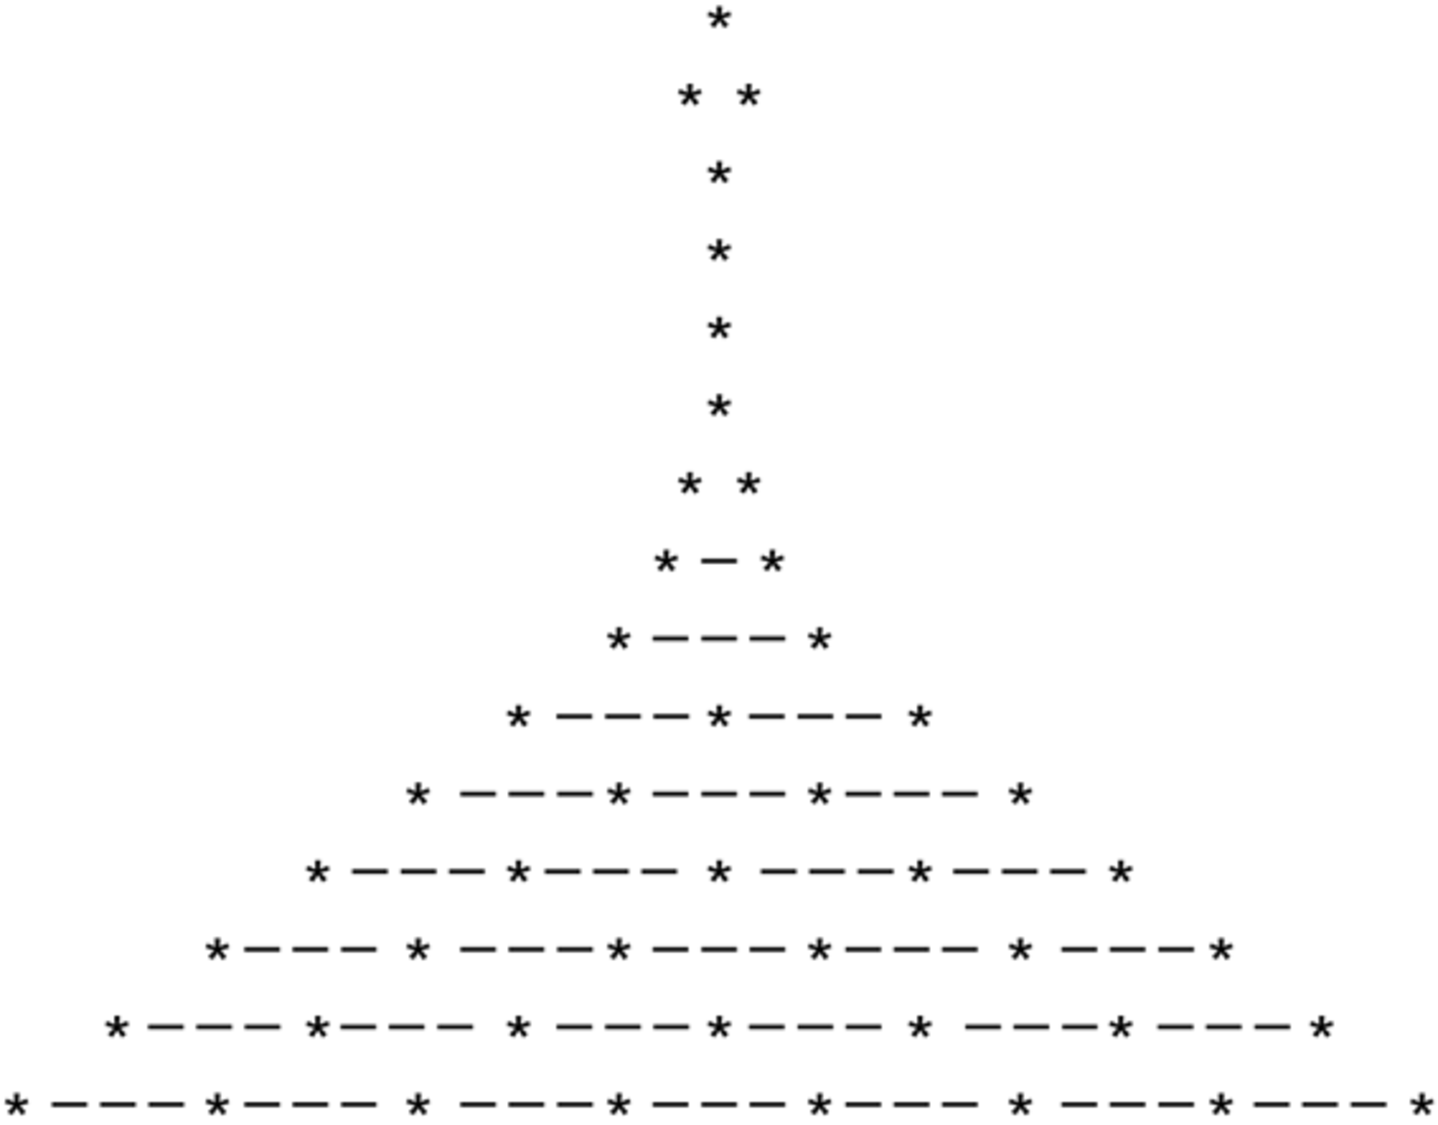
\includegraphics[keepaspectratio]{./media/OEBPS/Images/img_Dialog08_1.png}}

\end{center}

\chapter{螃蟹卡农}

周末在公园散步时，乌龟碰巧遇见了阿基里斯。

\dialogname{乌龟：}周末愉快，阿基。

\dialogname{阿基里斯：}彼此彼此。

\dialogname{乌龟：}同你在一起总是令人高兴的。

\dialogname{阿基里斯：}我也有同感。

\dialogname{乌龟：}在这样的天气里散步真是好极了，我宁愿散步回家。

\dialogname{阿基里斯：}哦，是吗？我觉得对你来说再没有比散步更好的了。

\dialogname{乌龟：}哎，阿基，这些天你看上去气色很好。

\dialogname{阿基里斯：}非常感谢。

\dialogname{乌龟：}不，不。来，尝尝我的荷兰雪茄吧。

\dialogname{阿基里斯：}啊，你在这方面真是个外行，你的口味不行。你不认为荷兰人的玩艺儿都很糟吗？

\dialogname{乌龟：}这点我可不同意。不过，说到口味，我终于看到了那位特别对你口味的艺术家艾舍尔的《螃蟹卡农》。那是有一天我在一家美术馆里看到的。我十分欣赏那种美和那种机巧：他把同一主题正向反向地罗织在一起。不过，我恐怕还是觉得巴赫要胜过艾舍尔。

\dialogname{阿基里斯：}这我不知道。但有一点可以肯定：我觉得讨论口味没劲。有句拉丁格言，恐怕你也知道：``口味无须争辩''。

\dialogname{乌龟：}告诉我，你这么大岁数了，觉得没劲了吗？

\dialogname{阿基里斯：}确切地说，是没多大力气了。

\dialogname{乌龟：}嗯，我也有这种感觉。

\dialogname{阿基里斯：}要是腿没力气了，就得拄手杖了。

\dialogname{乌龟：}你走路不使手杖吗？

\dialogname{阿基里斯：}我的一个朋友，他一向使。呆瓜。不过，我可从不沾惹手杖一根毛。

（突然，螃蟹不知从哪儿冒了出来，用爪子指着一只青肿凸起的眼睛，神情激动地踅来踅去。）

\dialogname{螃蟹：}好啊！好啊！怎么回事？怎么啦？你们瞧瞧这块青、这块肿，是一莽汉把我伤。嘿，而且是在这样一个好天里。你们瞧，我正在公园里懒洋洋地闲逛，迎面看到一个从彼得堡来的大块头------简直就是头熊------拿着一只吓人的俄国手杖。他足有三米高，除非我见了鬼。他那只手杖在地上划来划去，要不是我眼疾腿快，准被它打着了。于是我朝他爬过去，伸出爪子，打算拍拍他的膝盖，说，``对不起，先生，您用您的手杖把我们的公园老毛子化了。''可是，唔！他毫无幽默感------哪怕一丁、哪怕一星------噗！------他还放肆地敲了我一家伙，打在我眼睛上！按照我的本性，我原是横行无忌的，只是由于我们蟹类历来的传统，我原路退回了。毕竟，我们向前走时，就是倒着走。这是由于我们的基因，你们知道，它们是绕在一起的。这总是使我感到奇怪：究竟哪个在先------螃蟹还是基因？这也就是说，``哪个在后------基因还是螃蟹？''我总是绕圈子，你们知道。毕竟，这是由于我们的基因。我们倒着走时，就是向前走。呜呼！噫嘻！我得快快活活地颠儿了------在这样一个好天里。嘿，为螃蟹的生活叫好吧！再会！啊好！\kaitismall{（他像出现时一样突然地消失了。）}

\dialogname{乌龟：}我的一个朋友。他一向是呆瓜。不过我可从不沾惹老毛子的手杖。

\dialogname{阿基里斯：}你走路不使手杖吗？

\dialogname{乌龟：}要是腿没力气了，就得拄手杖了。

\pandocbounded{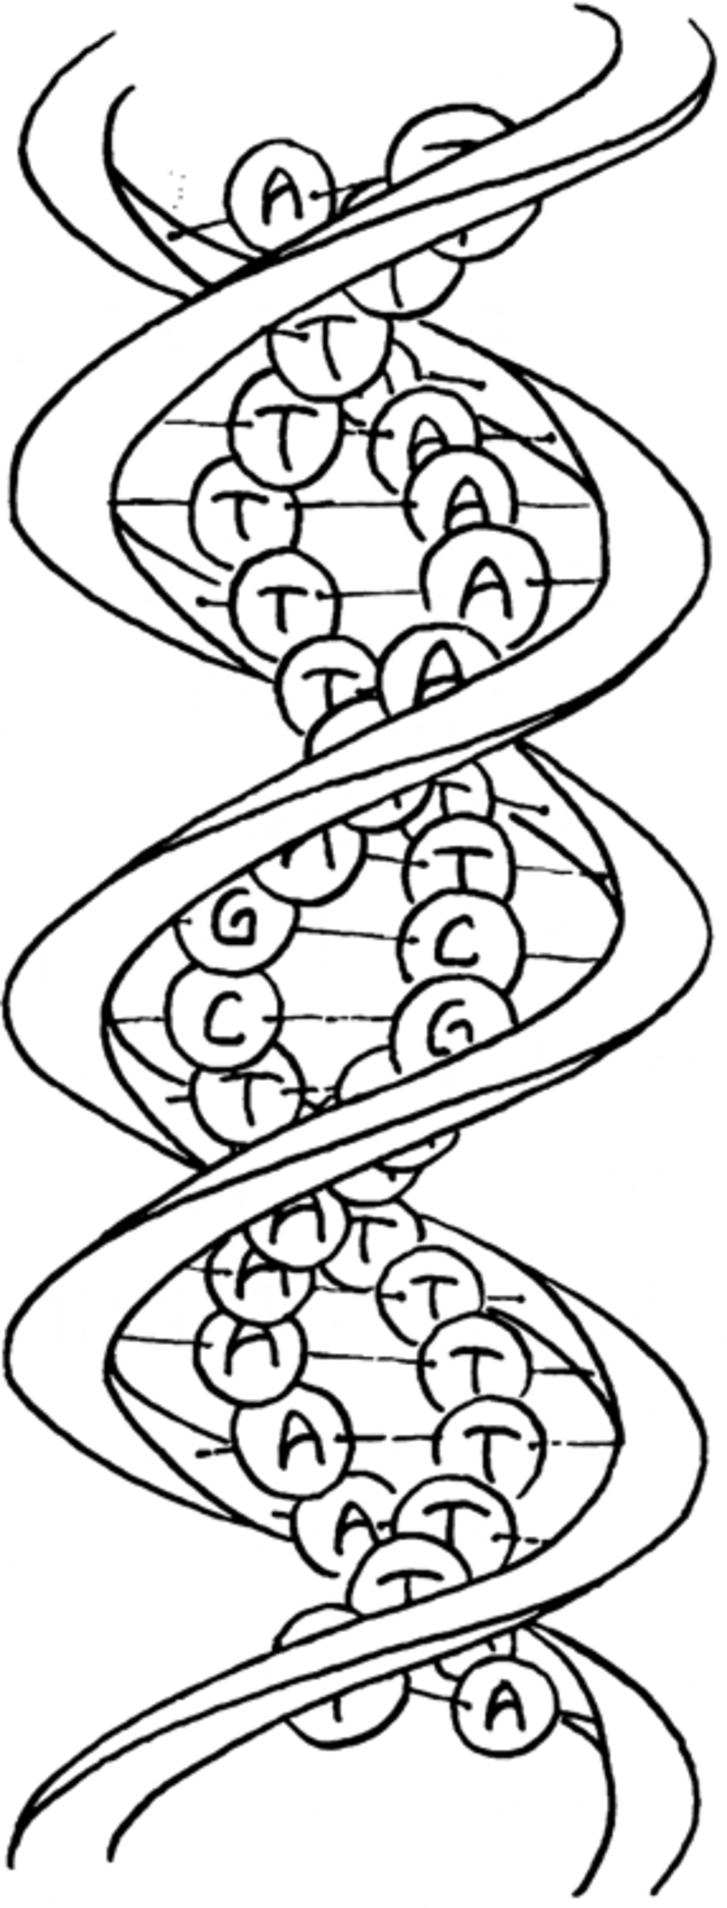
\includegraphics[keepaspectratio]{./media/OEBPS/Images/img_043.png}}

图43．螃蟹的一种基因中的一小段

它们一圈圈地缠绕着。当两股DNA链被拆开并且并排铺开时，它们读起来是这样的：

\ldots TTTTTTTTTCGAAAAAAAAA\ldots{}

\ldots AAAAAAAAAGCTTTTTTTTT\ldots{}

请注意它们是一模一样的，只是两者的走向正相反，一个前行时，另一个正好倒行。这正是音乐中所谓的``螃蟹卡农''这种形式所具有的特征。虽然不尽相同，它还是令人联想起回文来。回文就是一种正着读和倒着读都一模一样的句子。在分子生物学中，这样的DNA片段被称为``回文''------这种称呼有点用词不当，因为称它为``螃蟹卡农''要来得更准确些。不仅这个DNA片段是这样------而且本篇对话结构编排的基本序列也是螃蟹卡农式的。注意，在英文中，``阿基里斯''{[}Achilles{]}的第一个字母是A，``乌龟''{[}Tortoise{]}是T，``螃蟹''{[}Crab{]}是C，G则是``基因''{[}Gene{]}的第一个字母。

\dialogname{阿基里斯：}嗯，我也有这种感觉。

\dialogname{乌龟：}确切地说，是没有多大力气了。

\dialogname{阿基里斯：}告诉我，你这么大岁数了，觉得没劲了吗？

\dialogname{乌龟：}这我不知道。但有一点可以肯定：我觉得讨论口味没劲。有句拉丁格言，恐怕你也知道：``口味无须争辩''。

\dialogname{阿基里斯：}这点我可不同意。不过，说到口味，我终于听到了那位特别对你口味的作曲家巴赫的《螃蟹卡农》。那是有一天我在一次音乐会上听到的。我十分欣赏那种美和那种机巧：他把同一主题正向反向地罗织在一起。不过，我恐怕还是觉得艾舍尔要胜过巴赫。

\pandocbounded{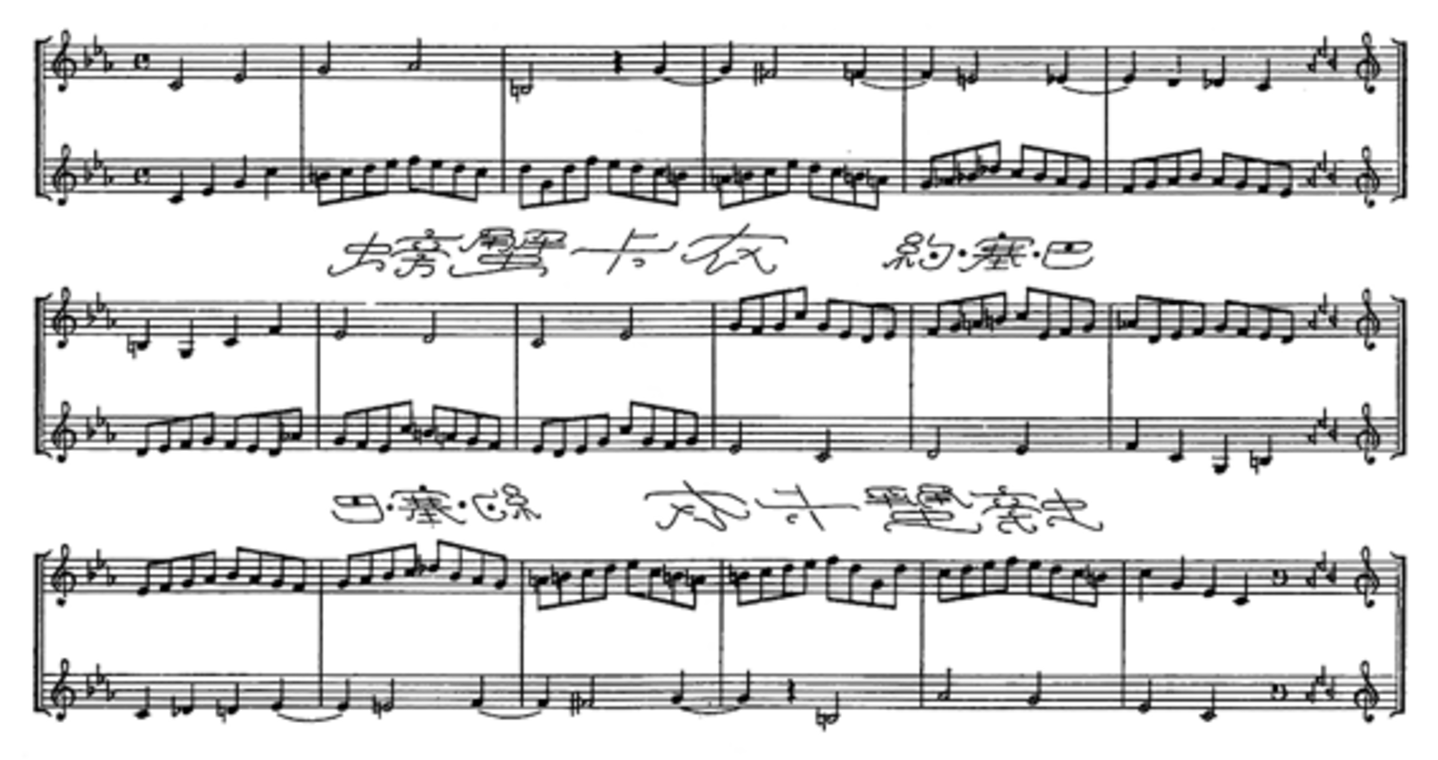
\includegraphics[keepaspectratio]{./media/OEBPS/Images/img_044.png}}

图44．螃蟹卡农

选自巴赫《音乐的奉献》{[}乐谱是用唐纳德·伯德的程序``斯马持''印制的，美术字由陈春光设计{]}

\dialogname{乌龟：}啊，你在这方面真是个外行，你的口味不行。你不认为荷兰人的玩艺儿都很糟吗？

\dialogname{阿基里斯：}不，不。来，尝尝我的荷兰雪茄吧。

\dialogname{乌龟：}非常感谢。

\dialogname{阿基里斯：}哎，龟兄，这些天你看去气色很好。

\dialogname{乌龟：}哦，是吗？我觉得对你来说再没有比散步更好的了。

\dialogname{阿基里斯：}在这样的天气里散步真是好极了，我宁愿散步回家。

\dialogname{乌龟：}我也有同感。

\dialogname{阿基里斯：}同你在一起总是令人高兴的。

\dialogname{乌龟：}彼此彼此。

\dialogname{阿基里斯：}周末愉快，龟兄。

\begin{center}

\pandocbounded{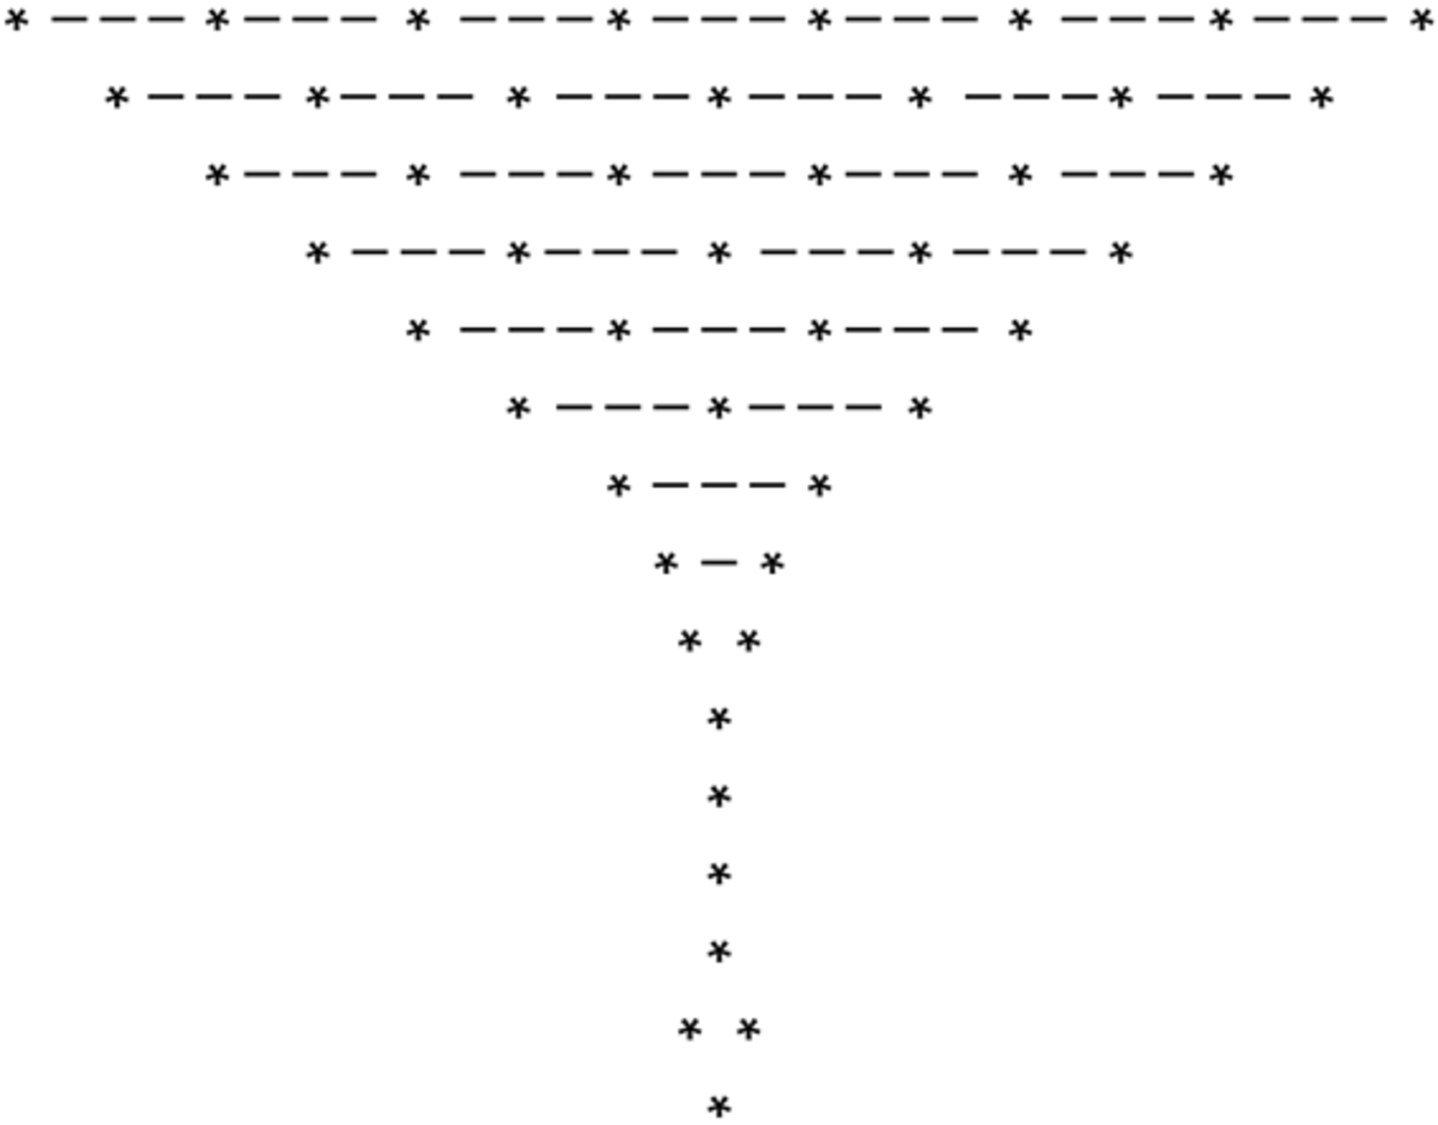
\includegraphics[keepaspectratio]{./media/OEBPS/Images/img_Dialog08_2.png}}

\end{center}

\phantomsection\label{Chapter08.xhtml}{}

第八章

\chapter{印符数论}

螃蟹卡农和间接自指

对话《螃蟹卡农》中出现了三个间接自指的例子。阿基里斯和乌龟都描述他们所熟知的艺术作品------而那些作品却很偶然地恰好与他们所处的对话具有同样的结构。（你可以想象当我------对话的作者------注意到这一点的时候，该是多么惊讶！）而且，螃蟹描述了一个生物学的结构，也是具有同样的性质。当然，有人可能读了这个对话，理解了它，同时却没能注意到这对话本身也具有一个螃蟹卡农的形式。这就是只在一个层次上来理解它，而忽视了另外的层次。要想看出自指，必须即看到这个对话的内容，也看到它的形式。

在这一章里，我们将定义一个形式系统------印符数论，也就是把数论表示在印刷符号中。这个系统简称为TNT，这一方面是因为英文的``印符数论''是Typographical Number Theory，而另一方面是因为这个形式系统能释放出很强的能量。哥德尔的构造就不仅要依靠对这个形式系统中串的内容所作的描述，还要依靠对这些串的形式所作的描述。一个意想不到的回旋是：由于哥德尔所发现的奇妙的映射，串的形式能在这个形式系统自身里面描述。现在就让我们来熟识一下这个具有转圈绕弯本领的奇特系统。

我们希望在TNT中都能表示些什么

我们先列举一些数论里典型的句子，然后想法找一集基本的概念，使所有那些句子都可以用这些概念重新叙述出来。下一步再把这些概念一个一个地赋予符号。顺便说明，我们从一开始就得清楚，``数论''这个术语仅仅只涉及正整数和零（以及这样的整数的集合）的性质。这些数被称为自然数。负数在这个理论中没有位置。所以，当用到``数''这个词时，它仅意味着自然数。下面这一点对读者来说是很重要的------极其重要的：在你心里始终要区别开我们的形式系统（TNT），和那个比较起来规定得不是那么明确，然而却是令人感到舒适的古老的数学分支，即数论本身。后者我将称之为``N''。

N------即数论------中的一些典型的句子是：

⑴．5是素数。

⑵．2不是平方数。

⑶．1729是两个立方数的和。

⑷．没有两个正立方数的和本身又是一个立方数。

⑸．存在有无穷多个素数。

⑹．6是偶数。

现在看起来，似乎对每一个诸如``是素数''或``是立方数''或``正的''这样的概念，我们都需要有一个符号------但是这些概念其实并非最基本的。例如，素数性是与一个数所具有的因子有关的，而这些因子又与乘法有关。立方性同样要通过乘法来定义。那么，就让我们来重新叙述一下这些句子，这回用那些看起来更为初等的概念。

⑴\textquotesingle．不存在这样的数a和b：它们都大于1，而且5等于a乘b。

⑵\textquotesingle．不存在一个数b，使得b乘以b等于2。

⑶\textquotesingle．存在数b和c，使得：b乘以b乘以b，加上c乘以c乘以c，等于1729。

⑷\textquotesingle．对任何大于0的数b和c，不存在数a，使得a乘以a乘以a等于b乘以b乘以b加上c乘以c乘以c。

⑸\textquotesingle．对每个数a，存在一个大于a的数b，具有这样的性质：不存在大于1的数c和d，使得b等于c乘以d。

⑹\textquotesingle．存在一个数e，使得2乘以e等于6。

这种分析已经使我们大大接近了得到数论语言的基本成分。很清楚，有少数短语反复地出现：

对任何数b

存在一个数b，使得\ldots\ldots{}

大于　　等于　　乘以　　加上

0, 1, 2, 3\ldots\ldots{}

这些短语的绝大部分都将被赋予单个的符号。一个例外是``大于''，它还能再进一步归约。事实上，句子``a大于b''可以变成

存在一个不等于0的数c，使得a等于b加上c。

数字

我们将不是对每一个自然数都赋予一个不同的符号。相反，我们将用一个非常简单、始终如一的方法，为每个自然数给出一个复合的符号------像我们在pq系统里做过的那样。下面是我们对自然数的记法：

\begin{longtable}[]{@{}ll@{}}
\toprule\noalign{}
\endhead
\bottomrule\noalign{}
\endlastfoot
零： & 0 \\
一： & S0 \\
二： & SS0 \\
三： & 　SSS0 \\
\multicolumn{2}{@{}l@{}}{%
等等} \\
\end{longtable}

符号S有一个解释------是它后面的那个东西``的后继''。因此，SS0的解释按字面上就是``零的后继的后继''。这种形式的串被称为数字。

变元和术语

显然，我们需要有一个方法来表示那些非指定的数------或者说可变的数。为此，我们将使用字母a、b、c、d、e。但就这五个是不够的。我们需要有一个无限制的供应方法，就像我们对命题演算中的原子所做的一样。我们将用一个相类似的方法去制造更多的变元：在数上面加撇。举例来说：

e

d\textquotesingle{}

c"

b"\textquotesingle{}

d""

都是变元。

从某种角度来说，用字母表的前五个字母多少是种奢侈，因为我们本可以只用a和撇号就行了。后面，我将真的不用b、c、d和e，结果将得到TNT的一种``简朴的''版本------此处所谓的``简朴''是说读懂复杂的公式变得较难了。不过当前我们还是奢侈一点。

那么，加法和乘法怎么办呢？非常简单：我们用习惯的符号``+''和``•''。然而，我们还要引进一个关于打括号的要求（我们现在正慢慢地滑入定义TNT良构串的规则中）。例如，要写``b加上c''和``b乘以c''，我们用这样的串

(b+c)

(b•c)

对这样的括号不能马虎。违反了这个约定就会产生一个不良构的公式（``公式''？我用这个术语来代替``串''，是因为习惯上是这样做的。一个公式不多不少就是TNT的一个串）。

顺带说一下，加法和乘法总是被认为是二元运算------也就是它们只把两个数联结起来，而从来不把三个或更多的数联结起来。因此，如果你希望去翻译``1加2加3''，你必须判定下面两个表达式中哪一个是你想要的：

(S0+(SS0+SSS0))

((S0+SS0)+SSS0)

下一个我们将要符号化的概念是等于。这非常简单：我们用``=''。直接把在N------非形式的数论------中所用的标准符号拿来的好处是明显的：容易读懂。而缺点则类似于对几何作形式处理时使用``点''和``线''这些词：除非一个人头脑非常清楚并仔细小心，否则他会很容易把词的普通意义与形式符号的严格受规则管辖的行为相混淆。在讨论几何时，我把形式术语写成黑体，以示日常用词与形式术语之间的区别。于是，在椭圆几何里，一个点是两个普通的点的结合体。但在这里，我们没有作这样的区分。因此需要特别小心，不要混淆一个符号与随它而来的所有联想。参考一下pq系统：像我以前说过的，``-\/-\/-''这个串不是3这个数，但它起着与3同构的作用，至少在加法的范围里是这样。对串SSS0可以做类似的说明。

原子与命题符号

命题演算的所有符号，除了用于构成原子的字母（P、Q和R）之外，都将在TNT中使用，并且仍然保持它们的解释。原子的角色将由这样的串来充当：当它们解释出来时，是一些关于相等的陈述，诸如S0=SS0或（S0·S0）=S0。现在，我们已经有了足够的准备来做一些从简单句子到TNT记号的翻译了：

2加3等于4：(SS0+SSS0)=SSSS0

2加2不等于3：～(SS0+SS0)=SSS0

如果1等于0，那么0等于1：＜S0=0→0=S0＞

这些串当中的第一个是原子，其余的都是复合公式。

自由变元与量词

上述所有的良构公式都具有这样的性质：它们的解释是句子，而这些句子不是为真，就是为假。但有的良构公式却不具有这个性质，比如这一个：

(b+S0)=SS0

它的解释是``b加1等于2''。由于b是未指定的，没有办法为这个陈述指派一个真值。它像一个含有代词的脱离了上下文的语句，例如``她很笨拙''。它既不真也不假，它等着读者把它放进一个上下文中去。正因为它既不真也不假，这样的公式就被称为开公式，而变元b则称为自由变元。

有一个办法能把一个开公式改变成一个闭公式，或者说句子。这个办法就是在它前面加一个量词------或者是短语``存在一个数b，使得\ldots\ldots''，或者是短语``对任何数b''。在第一种情况下，你得到的句子是

存在一个数b，使得b加1等于2。

显然这是真的。在第二种情况下，你得到的句子是

对任何数b，b加1等于2。

显然这是假的。我们现在来为这两种量词引进符号。这些句子翻译成TNT记号就是下面这样：

\gebfont{∃}b:(b+S0)=SS0{（``\gebfont{∃}''代表``存在''）}

\gebfont{∀}b:(b+S0)=SS0{（``\gebfont{∀}''代表``任何''或``所有的''）}

一定要注意，这些陈述不再是关于未指定的数了。第一个陈述是一个存在断言，而第二个是一个全称断言。即便用c而不是b来写它们，也还是意味着同样的事情：

\gebfont{∃}c:(c+S0)=SS0

\gebfont{∀}c:(c+S0)=SS0

在量词管辖之下的变元称为一个量化变元。下面的两个公式说明了自由变元与量化变元之间的区别：

\begin{longtable}[]{@{}ll@{}}
\toprule\noalign{}
\endhead
\bottomrule\noalign{}
\endlastfoot
(b·b)=SS0 & （开的） \\
～\gebfont{∃}b:(b·b)=SS0 & （闭的，是一个TNT的句子） \\
\end{longtable}

第一个公式表达了可能为某个自然数所具有的一个性质。当然，没有任何自然数具有这个性质。而这正是由第二个公式表达出来的。理解这两者之间的下列区别是很关键的：一个是带自由变元的串，它表达了一个性质，而另一个串里的变元是量化的，它表达了一个真实或虚假断言。至少带一个自由变元的公式------开公式------翻译成自然语言后就称为谓词。它是一个不带主语的句子（或者是这样的句子，它的主语是一个脱离上下文的代词）。例如，

\begin{itemize}
\tightlist
\item
  ``是一个不带主语的句子''
\item
  ``会是一个反常现象''
\item
  ``同时朝后和朝前跑''
\item
  ``一经请求就即席演奏六声部赋格''
\end{itemize}

都是非算术的谓词。它们所表达的性质，对具体的事物来说可以具有，也可以不具有。人们当然也可以坚持``哑主语''概念，比如``某某''。一个带自由变元的串就像一个用``某某''来当作其主语的谓词。例如，

(S0+S0)=b

就像是在说``1加上1等于某某''。这是一个带变元b的谓词。它表达了数b可以具有的一个性质。如果有人用各种各样的数字去替换b，他就会得到一连串公式，其中的大部分都将表达``假理''。下面是关于开公式与句子之间的区别的另一个例子：

\gebfont{∀}b:\gebfont{∀}c:(b+c)=(c+b)

当然，这个公式是一个表示加法交换律的句子。相反，

\gebfont{∀}c:(b+c)=(c+b)

却是一个开公式，因为b是自由的。它表达了未指定的数b可以具有，也可以不具有的一个性质------即，与所有的数c可交换。

翻译我们的例句

这样，我们的词汇表就全了。我们将以此来表达所有的数论语句！得有大量的实践才能掌握这些本领：如何用这种记法去表达N中复杂的陈述，以及倒过来，如何给出良构公式的意义。为此，我们还回到开始那六个例句，想法给出它们的TNT翻译。顺便说说，不要以为下面给出的翻译是唯一的------远不是如此。每一个句子都能由许多------无穷多的------方法来表达。

我们从最后的一个：``6是偶数''开始。这个例句我们用更初等的概念重述出来就成了``存在一个数e，使得2乘以e等于6''。这很容易：

\gebfont{∃}e:(SS0·e)=SSSSSS0

注意必须有量词。仅仅像下面这样写是绝对不行的：

(SS0·e)=SSSSSS0

这个串的解释当然既不真也不假，它只是表达了数e可以具有的一个性质。

奇怪的是，因为我们知道乘法是可交换的，于是我们可以很容易地就把上式写成：

\gebfont{∃}e:(e·SS0)=SSSSSS0

或者，知道相等是一个对称关系，我们换一下次序去写等式的两边：

\gebfont{∃}e:SSSSSS0=(SS0·e)

现在，关于``6是偶数''的这三个翻译是完全不同的串，而且还有一件事也绝不是显然的：它们之中任何一个是否是定理，受到其它任何一个是否是定理的制约（但是-\/-p-q-\/-\/-是定理这个事实，几乎一点也不依赖下面这一事实：其``等价的''串-p-\/-q-\/-\/-得是个定理。因为，作为人，这种等价性是在我们的心里，所以我们几乎是自动地去想到解释，而不考虑公式的结构方面的性质）。

我们可以很快解决句子2：``2不是一个平方数''，它的翻译几乎立刻就可以写出来：

～\gebfont{∃}b:(b·b)=SS0

然而，我们又一次发现了歧义。如果我们选用下面这种写法将如何呢？

\gebfont{∀}b:～(b·b)=SS0

第一种写法是说，``不存在一个数b，具有这样的性质，b的平方是2''，而第二种写法是说，``对任何数b，b的平方不是2。''再一次地，在我们看来，它们在概念上是等价的------但是对TNT来说，它们是不同的串。

我们接着来看句子3：``1729是两个立方数的和''。这次的翻译要含有两个存在量词，一个跟在另一个后面，如下所示：

\pandocbounded{
\includegraphics[keepaspectratio]{./media/OEBPS/Images/Formula15.png}}

还有许多其它可采用的写法。颠倒量词的次序；交换等式的两边；换变元为d和e；颠倒相加的次序；以不同方式相乘；等等，等等。不过，比较起来我更喜欢下面这两种翻译：

\gebfont{∃}b:\gebfont{∃}c:(((SSSSSSSSSS0·\\
SSSSSSSSSS0)·SSSSSSSSSS0)\\
+((SSSSSSSSS0·SSSSSSSSS0)\\
·SSSSSSSSS0))\\
=(((b·b)·b)+((c·c)·c))

和

\gebfont{∃}b:\gebfont{∃}c:(((SSSSSSSSSSSS0·\\
SSSSSSSSSSSS0)·SSSSSSSSSSSS0)\\
+((S0·S0)·S0))\\
=(((b·b)·b)+((c·c)·c))

你看出来是为什么了吗？

这一行中的窍门

现在我们来对付与此相关的句子4：``没有两个正立方数的和本身又是一个立方数''。假设我们只是要表述``7不是两个正立方数的和''。做这件事最简单的方法是，把断定7是两个正立方数的和的公式加以否定。这很像前面那个含1729的句子，只是我们在此必须加进去这样的条件：那两个立方数是正的。对付这个问题的窍门是在变元的前面加符号S，如下所示：

\gebfont{∃}b:\gebfont{∃}c:SSSSSSS0\\
=(((Sb·Sb)·Sb)+((Sc·Sc)·Sc))

你看，我们不是用b和c做立方，而是用它们的后继，那一定是正的，因为不论b还是c，能取的最小值就是零。于是，右边就表示两个正立方数的和。附带说一下，要注意当把短语``存在有数b和c使得\ldots\ldots''翻译出来时，并不包含代表``和''的符号``∧''。这个符号只是用来连接整个的良构串，而不是用于结合两个量词的。

现在我们已经翻译了``7是两个正立方数的和''，我们希望否定它。这只要在整个东西前边加一个弯号。（注意：虽然想要的短语是说``不存在数b和c使得\ldots\ldots''但你不要把每个量词都否定）于是我们得到：

～\gebfont{∃}b:\gebfont{∃}c:SSSSSSS0\\
=(((Sb·Sb)·Sb)+((Sc·Sc)·Sc))

可是我们原本要断言的性质不是对7而言的，而是对所有的立方数。因此，让我们把公式中的数字SSSSSSS0换成串（（a·a）·a），它是``a的立方''的翻译：

～\gebfont{∃}b:\gebfont{∃}c:((a·a)·a)\\
=(((Sb·Sb)·Sb)+((Sc·Sc)·Sc))

目前这个阶段，我们拥有一个开公式，因为其中的a是自由的。这个公式表达了一个数a可以具有也可以不具有的一个性质------而我们的目的是要断言所有的数都具有这个性质。这很简单------只要在整个东西前面加上一个全称量词：

\gebfont{∀}a:～\gebfont{∃}b:\gebfont{∃}c:((a·a)·a)\\
=(((Sb·Sb)·Sb)+((Sc·Sc)·Sc))

一个同样好的翻译是：

～\gebfont{∃}a:\gebfont{∃}b:\gebfont{∃}c:((a·a)·a)\\
=(((Sb·Sb)·Sb)+((Sc·Sc)·Sc))

在简朴的TNT中，我们可以用a\textquotesingle 来代替b，a"代替c，于是这个公式将成为：

～\gebfont{∃}a:\gebfont{∃}a\textquotesingle:\gebfont{∃}a":((a·a)·a)\\
=(((Sa\textquotesingle·Sa\textquotesingle)·Sa\textquotesingle)+((Sa"·Sa")·Sa"))

那么句子1：``5是素数''又怎么样呢？我们已经把它改写成了这个样子：``不存在数a和b，它们都大于1，使得5等于a乘以b''。我们可以将它稍加改变如下：``不存在数a和b，使得5等于a加上2，再乘以b加上2''。这又是一招------因为a和b被限定只能取自然数值，所以这种方法同样也是可行的。现在，``b加上2''可以翻译成(b+SS0)，但是还有一个更为简短的写法------SSb。同样，``c加上2''可以写成SSc。现在，我们的翻译非常的简洁：

～\gebfont{∃}b:\gebfont{∃}c:SSSSS0=(SSb·SSc)

如果没有前面的弯号，它就是断言这样的两个自然数存在：当它们分别增加2之后，其乘积等于5。带上前面的弯号，整个陈述就被否定了，结果就成了断言：5是素数。

如果我们想断言d加e加1是素数，而不说5，那么，最经济的方法是用串（d+Se）来替换代表5的那个数字：

～\gebfont{∃}b:\gebfont{∃}c:(d+Se)=(SSb·SSc)

又一次，得到一个开公式，它的解释是一个既不真也不假的句子，它只是一个关于两个未指定的数d和e的断言。注意，用串（d+Se）来表示的数必然是大于d的，因为已经为d加上了一个虽然是未指定的但一定是正的数值。因此，如果我们在变元e上进行存在性的量化，我们将得到一个公式来断言：

存在一个数，它大于d，并且它是素数。

\gebfont{∃}e:～\gebfont{∃}b:\gebfont{∃}c:(d+Se)=(SSb·SSc)

好，我们现在剩下要做的全部事情就是要断言：不管d是什么，这个性质实际上总是有的。做这件事的方法是在变元d上进行全称性的量化：

\gebfont{∀}d:\gebfont{∃}e:～\gebfont{∃}b:\gebfont{∃}c:(d+Se)=(SSb·SSc)

这正是句子5的翻译！

翻译习题

这样，我们就完成了六个典型数论句子的翻译练习。但是，这并不一定就使你成了一个使用TNT记号的专家。还有一些技巧需要掌握。下面的六个良构公式可以检验你对TNT记法的理解。它们的意思是什么？哪些是真的（当然，是在解释之下），哪些是假的？（提示：对付这个练习的方法是逐步向左移。首先，翻译原子；其次，想出加上一个单个的量词或一个弯号会对翻译起什么作用；然后向左移，加上另一个量词或弯号；然后再向左移，再做同样的事情。）

～\gebfont{∀}c:\gebfont{∃}b:(SS0·b)=c

\gebfont{∀}c:～\gebfont{∃}b:(SS0·b)=c

\gebfont{∀}c:\gebfont{∃}b:～(SS0·b)=c

～\gebfont{∃}b:\gebfont{∀}c:(SS0·b)=c

\gebfont{∃}b:～\gebfont{∀}c:(SS0·b)=c

\gebfont{∃}b:\gebfont{∀}c:～(SS0·b)=c

第二个提示：或者它们中有四个为真两个为假，或者有四个为假两个为真。）

怎样区分真和假？

到了这个时候，值得停一下好好想一想：一个能筛选出真公式与假公式的形式系统是什么意思。这个系统要去处理所有这些串------它们在我们眼里像是陈述------它们作为一种制品只有形式，没有内容。并且这个系统要像一个筛子一样，只能通过那些带有特殊样式------``真理样式''------的制品。如果你自己已经走通了上述六个公式，并且考虑了它们的意义，从而分离了真的和假的，你将领略到这种系统必须要具有的那种精妙之处，它们能够做同样的事情------但却是印符地来做！用来区分真陈述集合与假陈述集合的界线（用TNT记法写成）绝不是笔直的；这个分界线有着许多莫测的弯曲（回想一下图18），数学家们在这里和那里描绘其走向，一直工作了好几百年。不难想象，如果有一个印符的方法，能保证把任何一个公式放到这分界线的适当的一边，那该多棒！

关于良构性的规则

有一张良构公式的形成规则表是必要的。下面就给出这张表。先要做些准备，定义数字、变元和项。这三种类型的串是良构公式的组成成分，但仅就它们本身还谈不上良构。最小的良构公式是原子；然后有一些将原子结合起来的规则。这些规则中，有许多是递归加长规则，它们把某个给定种类的东西作为输入，产生出同一种类的长一些的东西。在这张表里，我用``x''和``y''代表良构公式，而用``s''\,``t''以及``u''去代表其他种类的TNT串。不用说，这五个符号没有一个本身是TNT的符号。

数字：

0是一个数字。

一个前面加上了S的数字仍是一个数字。

例子：0　　S0　　SS0　　SSS0　　SSSS0　　SSSSS0

变元：

a是一个变元。如果我们不限于简朴版本，那么b，c，d以及e同样也都是。

一个加了一撇的变元仍是一个变元。

例子：a　　b\textquotesingle{}　　c"　　d"\textquotesingle{}　　e""

项：

所有数字和变元都是项。

一个前面加了S的项仍是一个项。

如果s和t都是项，那么(s+t)和(s·t)也同样都是项。

例子：0　　b　　SSa\textquotesingle{}　　(S0·(SS0+c))　　S(Sa·(Sb·Sc))

项可以分成两类：

⑴．\heititext{确定项}。这些项不包含变元。

例子：0　　(S0+S0)　　SS((SS0·SS0)+(S0·S0))

⑵．\heititext{非确定项}。这些项包含有变元。

例子：b　　Sa　　(b+S0)　　(((S0+S0)+S0)+e)

以上的规则是告诉我们如何制作良构公式的部件，下面的规则是告诉我们如何去制作完整的良构公式。

原子：

如果s和t是项，那么s=t是一个原子。

例子：S0=0　　(SS0+SS0)=SSSS0　　S(b+c)=((c·d)·e)

如果一个原子中含有一个变元u，那么u在它里面是自由的。所以在上面最后一个例子里有四个自由变元。

否定：

一个前面加了一个弯号的良构公式是良构的。

例子：～S0=0　　～\gebfont{∃}b:(b+b)=S0　　～＜0=0→S0=0＞～b=S0

一个变元的量化状况（就是说变元是自由的还是量化的）在否定之下并不改变。

复合：

如果x和y是良构公式，并且没有什么变元在它们中的一个里面是自由的而在另一个里面是量化的，那么下列都是良构公式：

＜x∧y＞，＜x∨y＞，＜x→y＞。

例子：＜0=0∧～0=0＞　＜b=b∨～\gebfont{∃}c:c=b＞　＜S0=0→\gebfont{∀}c:～\gebfont{∃}b:(b+b)=c＞

一个变元的量化状况在这种情况下不改变。

量化：

如果u是一个变元，x是一个良构公式，u在它里面是自由的，那么下面的串是良构公式：

\gebfont{∃}u:x和\gebfont{∀}u:x

例子：\gebfont{∀}b:　　\gebfont{∀}c:～\gebfont{∃}b:(b+b)=c～\gebfont{∃}c:Sc=d

开公式：含有至少一个自由变元。

例子：～c=c　　b=b　　＜\gebfont{∀}b：b=b∧～\gebfont{∃}c=c＞

闭公式（句子）：不含自由变元。

例子：S0=0　　～\gebfont{∀}d:d=0　　\gebfont{∃}c:＜\gebfont{∀}b:b=b∧～c=c＞

这就完成了TNT良构公式的形成规则表。

再来几个翻译练习

现在，给你几个练习做，检验一下你对TNT记法的理解。试一试把下列N句子中的前四个翻译成TNT句子，把最后一个译成一个开的良构公式。

所有的自然数都等于4。

不存在等于它自身平方的自然数。

不同的自然数有不同的后继。

如果1等于0，那么每个数都是奇数。

b是2的某次方。

你可能发现最后的一个有点难对付。不过它和下一个一比，就小巫见大巫了：

b是10的某次方。

奇怪的是，这一个需要有极大的聪明机智才能翻译成我们的记法中的东西。我要告诫读者：只有在你乐意把几小时几小时的时间花在它上面------并且你还颇知道点数论的时候------再去尝试做这道题。

一个非印符系统

至此，我们结束了对TNT记法的说明，但我们还没有表明如何使TNT成为我们描述过的那个雄心勃勃的系统。这一点若是成功了，我们曾对各个符号做出的解释就会得到证实。不过，在我们做到之前，这些特定的解释并不比对pq系统的符号所作的``马-苹果-幸福''解释更有意义。

有人可能会建议按下列方法来构造TNT：（1）没有任何推理规则。它们是不必要的，因为（2）我们取数论的所有真语句（用TNT记法写成）来当作公理。多简单的处方！不幸的是，任何人一望即知这根本是空洞无物的说法。第（2）部分显然不是对串的一个印符描述。TNT的整个目的就是要确定：是否可能，以及如何印符地刻划所有对应于真理的串。

TNT的五条公理及第一组规则

于是，我们将遵循一条比上述建议困难得多的路线走下去：我们将有公理和推理规则。首先，按照约定，命题演算的全部规则都被接受进TNT里来。因此，下面这个式子将是TNT的一个定理：

＜S0=0∨～S0=0＞

推导出它的过程与推导＜P∨～P＞的过程是一样的。

在我们给出更多的规则之前，让我们先给出TNT的五条公理：

\heititext{公理1：}\gebfont{∀}a:～Sa=0

\heititext{公理2：}\gebfont{∀}a:(a+0)=a

\heititext{公理3：}\gebfont{∀}a:\gebfont{∀}b:(a+Sb)=S(a+b)

\heititext{公理4：}\gebfont{∀}a:(a·0)=0

\heititext{公理5：}\gebfont{∀}a:\gebfont{∀}b:(a·Sb)=((a·b)+a)

（在简朴的版本中，用a\textquotesingle 来代替b）。它们都很容易理解。公理1陈述了有关数0的一个特殊事实；公理2和3是关于加法的性质的；公理4和5是关于乘法的性质的，并且特别涉及到与加法的关系。

五条皮亚诺公设

顺便说说，公理1的解释------``零不是任何自然数的后继''------是自然数的五条著名的性质之一，这些性质是由数学家和逻辑学家朱·皮亚诺于1889年首次明确认定的。皮亚诺沿着欧几里德的路线提出他的公设，他的做法是：不去致力于把推理的原则加以形式化，而是力图给出一个自然数性质的小小的集合，从它出发，其余的每样东西都能由推理而得出。因此，皮亚诺的努力也许可以认为是``半形式化的''。皮亚诺的工作具有重要影响，所以，介绍一下皮亚诺的五条公设是会有好处的。由于``自然数''概念是一个皮亚诺设法去定义的东西，所以我们将不使用这个充满了内涵的熟悉的术语``自然数''。我们将用一个未经定义的术语``神怪''来替代它，这个术语是一个来得很新鲜的词，并且对我们来说这个词是没有内涵的。于是，皮亚诺的五条公设是在神怪上加了五条限制。另外还有两个未定义项：``怪物''与``元''，我留给你自己去想出它们是要表示通常的什么概念。五条皮亚诺公设是：

⑴．怪物是一个神怪。

⑵．每一个神怪有一个元（它也是一个神怪）。

⑶．怪物不是任何神怪的元。

⑷．不同的神怪有不同的元。

⑸．如果怪物有X，并且每个神怪都把X递送给它的元，那么所有的神怪都得到X。

在《和声小迷宫》中的那些灯的启发下，我们将把众神怪的集合命名为``\heititext{造物神}''。这又回到了盖奥尔格·康托尔的死对头，德国数学家和逻辑学家列奥波尔德·克罗内克的那句名言：``造物神造出了自然数，其余的一切都是人的事。''

你可能认出来了，皮亚诺的第五条公设就是数学归纳法原理------继承性论证的另一说法。皮亚诺希望他加在概念``怪物''、``神怪''以及``元''上的五条限制是如此之强，以至于如果两个不同的人在心里对这些概念形成意象，这两个意象会有完全同构的结构。举例来说，每个人的意象都会包括无穷多个不同的神怪。并且，大概每个人都会同意，没有一个神怪与它自身的``元''完全相同，或者与它的``元''的``元''完全相同，等等。

皮亚诺希望把自然数的本质纳入到他的五条公设之中。数学家们一般都承认他成功了，但是这并没有减少下面这个问题的重要性：``怎样区别关于自然数的真陈述和假陈述句？''为了回答这个问题，数学家们又转向完全形式化的系统，比如TNT。不管怎么说，你将在TNT中看到皮亚诺的影响，因为所有他的公设都以这样或那样的方式被引进到TNT里来了。

TNT中的新规则：特称和概括

现在我们来看TNT中的新规则。许多这种规则使我们能深入并改变TNT原子的内部构造。在这个意义上，它们是在和串的更``微观''的性质打交道，而不像命题演算的规则，把原子当作不可分割的单位。举例来说，我们想从第一条公理中抽出串～S0=0。为此，我们需要有一条规则使我们能去掉一个全称量词，同时，如果我们愿意，能改变剩下的串的内部构造。下面就是这么一条规则：

特称规则：假设u是一个出现在串x中的变元。如果串\gebfont{∀}u:x是一个定理，则x也是定理，并且，对x中的u做任何替换而得到串同样也都是定理，但不论u出现在什么地方，都要用同一个项去替换。

（限制：用来替换u的项必须不包含任何在x中被量化了的变元。）

特称规则使我们能把刚才那个串从公理1中提取出来。这是一个一步的推导：

\begin{longtable}[]{@{}ll@{}}
\toprule\noalign{}
\endhead
\bottomrule\noalign{}
\endlastfoot
\gebfont{∀}a:～Sa=0 & 公理1 \\
～S0=0 & 特称 \\
\end{longtable}

注意，特称规则将允许某些包含自由变元的公式（即开公式）成为定理。举例来说，用特称，下列的串也能从公理1导出：

～Sa=0

～S(c+SS0)=0

还有另一个规则，概括规则，使我们能把全称量词放回到一些定理中去------那些定理所含的变元由于以前使用了特称规则而成为自由的了。举例来说，把概括规则作用到上面的那两个串中的第二个，我们就得到：

\gebfont{∀}c:～S(c+SS0)=0

概括正好取消了特称的作用，反过来也一样。通常，概括总是用于某些中间步骤已经以各种各样的方式对开公式作了一番变换之后。下面是这条规则的严格叙述：

概括规则：假设x是一个定理，其中的变元u是自由出现的。那么\gebfont{∀}u:x是一个定理。

（限制：在一个幻想里面，不允许对任何自由出现在该幻想的前提中的变元作概括。）

在这两个规则上加限制的必要性很快就会清楚地表现出来。附带说一下，这个概括与第二章中提到过的欧几里德在证明素数有无穷多时所用的概括是一回事。我们已经可以看到，符号变换规则开始靠近数学家们所使用的那种推理了。

存在量词

刚才的两条规则说的是如何取走全称量词以及如何把它们放回去，下面的两条规则说的是如何处理存在量词。

互换规则：假设u是一个变元。那么串\gebfont{∀}u:～与～\gebfont{∃}u:在任何定理中的任何地方都是可互换的。

举个例子，让我们把这条规则应用到公理1：

\begin{longtable}[]{@{}ll@{}}
\toprule\noalign{}
\endhead
\bottomrule\noalign{}
\endlastfoot
\gebfont{∀}a:～Sa=0 & 　公理1 \\
～\gebfont{∃}a:Sa=0 & 　互换 \\
\end{longtable}

附带地，你可能注意到，这两个串都是``零不是任何自然数的后继''这个句子在TNT中的完美自然的表述。所以，它们能够容易地变来变去是一件好事。

下一条规则则更为直观了。它对应于非常简单的一种推理，即我们从``2是素数''到``存在一个素数''所做的推理。这条规则的名称是自明的：

存在规则：假设一个项（可以含有变元，只要是自由的）在一个定理中出现一次或多次。那么，这个项的任何（或者是一些，或者是所有）出现都可以用一个不在定理中出现的变元来替代（替代之后当然就在这个定理中出现了），相应的存在量词则必须放在最前面。

让我们------像往常一样------对公理1来应用这条规则：

\begin{longtable}[]{@{}ll@{}}
\toprule\noalign{}
\endhead
\bottomrule\noalign{}
\endlastfoot
\gebfont{∀}a:～Sa=0 & 　公理1 \\
～\gebfont{∃}b:\gebfont{∀}a:～Sa=0 & 　存在 \\
\end{longtable}

你现在可以试试根据迄今所给出的规则去调拨符号，产生出定理～\gebfont{∀}b:\gebfont{∃}a:Sa=b。

等号规则和后继规则

我们已经为变换量词给出了规则，但到目前为止还没有一个针对符号和``S''的规则。我们现在就来纠正这一状况。以下，r、s和t都代表任意的项。

等号规则：

对称：如果r=s是一个定理，那么s=r同样也是定理。

传递：如果r=s和s=t都是定理，那么r=t也是定理。

后继规则：

加S：如果r=t是一个定理，那么Sr=St是一个定理。

去S：如果Sr=St是一个定理，那么r=t是一个定理。

这些规则能够为我们提供极其丰富的各式各样的定理。比如，下列推导就产生出一些相当基本的定理：

\begin{longtable}[]{@{}lll@{}}
\toprule\noalign{}
\endhead
\bottomrule\noalign{}
\endlastfoot
⑴ & \gebfont{∀}a:\gebfont{∀}b:(a+Sb)=S(a+b) & 公理3 \\
⑵ & \gebfont{∀}b:(S0+Sb)=S(S0+b) & 特称（S0对a） \\
⑶ & (S0+S0)=S(S0+0) & 特称（0对b） \\
⑷ & \gebfont{∀}a:(a+0)=a & 公理2 \\
⑸ & (S0+0)=S0 & 特称（S0对a） \\
⑹ & S(S0+0)=SS0 & 加S \\
⑺ & （S0+S0）=SS0 & 传递（第3、6行） \\
\multicolumn{3}{@{}l@{}}{%
*　*　*　*　*} \\
⑴ & \gebfont{∀}a:\gebfont{∀}b:(a·Sb)=((a·b)+a) & 公理5 \\
⑵ & \gebfont{∀}b:(S0·Sb)=((S0·b)+S0) & 特称（S0对a） \\
⑶ & (S0·S0)=((S0·0)+S0) & 特称（0对b） \\
⑷ & \gebfont{∀}a:\gebfont{∀}b:(a+Sb)=S(a+b) & 公理3 \\
⑸ & \gebfont{∀}b:((S0·0)+Sb)=S((S0·0)+b) & 特称（(S0·0)对a） \\
⑹ & ((S0·0)+S0)=S((S0·0)+0) & 特称（0对b） \\
⑺ & \gebfont{∀}a:(a+0)=a & 公理2 \\
⑻ & ((S0·0)+0)=(S0·0) & 特称（(S0·0)对a） \\
⑼ & \gebfont{∀}a:(a·0)=0 & 公理4 \\
⑽ & (S0·0)=0 & 特称（S0对a） \\
⑾ & ((S0·0)+0)=0 & 传递（第8、10行） \\
⑿ & S((S0·0)+0)=S0 & 加S \\
⒀ & ((S0·0)+S0)=S0 & 传递（第6、12行） \\
⒁ & (S0·S0)=S0 & 传递（第3、13行） \\
\end{longtable}

非法的捷径

一个令人感兴趣的问题是：``怎样为串0=0做一个推导？''看起来，要走的路线显然会是先推出串\gebfont{∀}a:a=a，然后用特称。那么，下面这个\gebfont{∀}a:a=a的``推导''怎么样\ldots\ldots 有什么问题吗？你能把它修补好吗？

\begin{longtable}[]{@{}lll@{}}
\toprule\noalign{}
\endhead
\bottomrule\noalign{}
\endlastfoot
⑴ & \gebfont{∀}a:(a+0)=a & 　公理2 \\
⑵ & \gebfont{∀}a:a=(a+0) & 　对称 \\
⑶ & \gebfont{∀}a:a=a & 　传递（第2，1行） \\
\end{longtable}

我用这个小小的练习来指出一个简单的事实：在变换熟悉的符号（诸如``=''）时，不要跳得太快。你必须遵循规则，而不是你关于符号的被动意义的知识。当然，后一种知识在指引一个推导该走什么路线时是极有价值的。

为什么对特称和概括要加限制

现在让我们来看为什么对特称和概括二者都有加限制的必要性。下面有两个推导，两者当中都有一个限制被违反了。看看由此产生的灾难性后果：

\begin{longtable}[]{@{}lll@{}}
\toprule\noalign{}
\endhead
\bottomrule\noalign{}
\endlastfoot
⑴ & ［ & 推入 \\
⑵ & 　a=0 & 前提 \\
⑶ & 　\gebfont{∀}a:a=0 & 概括（错了） \\
⑷ & 　Sa=0 & 特称 \\
⑸ & {]} & 弹出 \\
⑹ & ＜a=0→Sa=0＞ & 幻想规则 \\
⑺ & \gebfont{∀}a:＜a=0→Sa=0＞ & 概括 \\
⑻ & ＜0=0→S0=0＞ & 特称 \\
⑼ & 0=0 & 以前的定理 \\
⑽ & S0=0 & 分离（第9，8行） \\
\end{longtable}

这是第一个灾难。另一个灾难是由于用错了特称而产生的。

\begin{longtable}[]{@{}lll@{}}
\toprule\noalign{}
\endhead
\bottomrule\noalign{}
\endlastfoot
⑴ & \gebfont{∀}a:a=a & 　以前的定理 \\
⑵ & Sa=Sa & 　特称 \\
⑶ & \gebfont{∃}b:b=Sa & 　存在 \\
⑷ & \gebfont{∀}a:\gebfont{∃}b:b=Sa & 　概括 \\
⑸ & Sa=Sa & 　特称（错了！） \\
\end{longtable}

因此，现在我们看到，为什么那些限制是必要的。

这里有一个简单的谜题：把皮亚诺的第四条公设翻译成为TNT记法（如果你还不曾这样做的话），然后把这个串当作一个定理而推导出来。

少了什么东西

现在，如果你用迄今所介绍过的TNT规则和公理四处试一会儿的话，你将发现，你可以产生出如下的定理金字塔（这是一个串的集合，所有这些串都是从同一个模子里翻铸出来的，相互之间仅有的不同是填在里边的数字分别为0、S0、SS0等等）；

\begin{longtable}[]{@{}lll@{}}
\toprule\noalign{}
\endhead
\bottomrule\noalign{}
\endlastfoot
(0+S0) & = & S0 \\
(0+SS0) & = & SS0 \\
(0+SSS0) & = & SSS0 \\
(0+SSSS0) & = & SSSS0 \\
\end{longtable}

事实上，这个塔中的每个定理都能从恰在它之上的那个定理中推出来，只需一两步。因此它是一种定理的``多级瀑布''，每一级触发下一级（这些定理很容易让人想起pq系统中的定理，在那里，左端和右端的短杠组是同时增长的）。

这里有一个我们能很容易地写下来的串，它概括地说出了它们作为整体时的被动意义。这个全称量化了的概述串是：

\gebfont{∀}a:(0+a)=a

用迄今为止所给出的规则，这个串还产生不出来。你若不信，可以自己试试。

你可能会认为，用如下的规则，我们立刻就可以扭转这个局面：

（草拟的）全规则：如果在一个金字塔中的所有的串都是定理，那么，用来概述它们的全称量化的串同样也是定理。

这条规则的问题是：它不能在J方式下使用。只有从外部对系统进行考察的人，才有可能知道串的一个无穷集合全都是定理。因此这不是一条可以安放到形式系统里去的规则。

ω不完全系统与不可判定串

于是我们发现我们处于奇怪的境地：我们能印符地产生关于任何特定的数之间相加的定理，但是像上面那样的一般地表达了加法性质的串，虽然那么简单明了，却不是一个定理。你可能觉得这并不那么奇怪，因为在pq系统里我们曾恰好就处于这种情境中。但是，pq系统并没有声称它该做到什么；并且，事实上，用它的符号体系也的确无法表示加法的一般性质，更不用说证明它们了。pq系统根本没有这样的装备，我们因而也就没想过那是它的缺陷。但在这里，表示能力要远远强得多了，所以我们相应地对TNT比对pq系统有更高的期望。如果上述的串不是一个定理，那么我们就有充分的理由认为TNT是有缺陷的。事实上，有一个名字是专为带有这种类型缺陷的系统准备的------称为``ω不完全性''（所谓``ω''------``欧米伽''------来自于这样的事实：自然数的全体有时候被记作``ω''）。下面是精确的定义：

{一个系统是ω不完全的，如果在一个金字塔中的所有串都是定理，而全称量化的概述串却不是一个定理。}

顺带地，上述概述串的否定------

～\gebfont{∀}a:(0+a)=a

------也不是TNT的定理。这意味着，原先的那个串在系统里是不可判定的。如果两者之一是定理，那么我们就说它是可判定的。虽然这听起来像是个神秘的术语，但一个给定的系统中的不可判定性是没有什么神秘的。它仅仅是该系统还能够扩充的一个标志。举例来说，在绝对几何学里，欧几里德的第五条公设是不可判定的。它必须作为一条特别的几何公设加进来，从而导致欧几里德几何学；或者相反，它的否定是能够加进来的，从而导致非欧几里德几何学。如果你回想一下几何学，你会记起为什么会出这种稀奇古怪的事情。这就是因为绝对几何学的四条公设没有固定住``点''和``线''这些术语的意义，从而为这些概念具有不同外延留下了余地。欧几里德几何学的点和线提供了``点''和``线''这些概念的一种外延；非欧几里德几何学的点和线则是提供另一种。然而，两千年来，使用先入为主的词``点''和``线''则使人相信那些词必须是单值的，只能有一个意义。

非欧几里德TNT

我们现在就TNT而言面临着一个类似的情况。我们曾沿用的记号使我们带上了某些成见。例如，使用符号``+''就使我们很容易地想：每个里面带有一个加号的定理都应该是在说那个已知的、熟悉的、``可感知''的、我们称为``加法''的运算的事情。因此，如果我们提出增加一个如下的``第六公理''，会让人觉得很是格格不入：

～\gebfont{∀}a:(0+a)=a

这与我们关于加法所持的观念不相适应。但这是我们迄今为止所描述的TNT的一个可能的扩充。采用它为其第六公理所得到的系统是一个一致的系统，就是说，不会同时有两个形式为x和～x的公式都是定理。然而，当你把这条``第六公理''与前面列出来的那个定理的金字塔并置在一起时，你也许会由于那个塔和这条新的公理之间的似乎不一致而感到困惑。但是，这种不一致性不像另一种（在那里x和～x二者都是定理）那么有害。事实上，这并非一个真正的不一致，因为存在有一种解释符号的方法，使每样事情结果都是顺理成章的。

ω不一致性与不一致性不是一回事

这种不一致性的产生是由于下面两件事的对立：（1）一个由一些定理组成的金字塔，它们集合起来断言所有的自然数具有某种性质，与（2）一个单个的定理，它看上去是断言并非所有的自然数具有该性质。我们称这种不一致性为ω不一致性。一个ω不一致的系统更像一个被人们``初拒后纳的''非欧几里德几何。为了能对这些东西形成一个心智上的模型，读者得想象存在有一些``额外的''，未曾料到的数------让我们不称它们为``自然''的，而称它们为``超自然''的数------它们都不具有相应的数字。因此，有关它们的事实不能在金字塔里表示出来。（这有一点像阿基里斯对造物神的想象------是一种``超神怪''，一种比任何神怪都大的东西。这曾遭到怪物的嘲笑，但这是一个合理的想象，并可以帮助你去想象超自然数）。

这就告诉了我们：迄今所介绍的TNT的公理和规则并没有完全固定住对TNT符号的解释。在一个人的心智模型中这些符号代表什么概念，这仍然还有种种变化的余地。这种种可能的外延中的每一个，都可以进一步固定住其中的某些概念，只是以不同的方式而已。如果我们加上上面的那个``第六公理''，那么哪些符号会带上被人们所``初拒''的那种被动意义？是所有这些符号都会染上，还是它们中的一些仍然会代表我们想让它们去代表的意义？我将让读者去考虑这个问题。在第十四章里我们会碰到一个类似的问题，然后再来讨论这件事。总而言之，我们现在不沿着这个扩充走，而是继续尝试去修补TNT的ω不完全性。

最后一条规则

``全规则''的问题是：它要求知道一个无穷高的金字塔中所有的行都是定理------这对一个有穷的主体来说是要求得太多了。但是让我们假设这个塔的每一行都能够用某种模式化的方法从它的前一行推出来。这样就能用一个有穷的推理去说明在塔里的所有的串都是定理。于是，技巧仅在于去找出造成多级瀑布的那个模式，并证明那个模式本身就是一个定理。这就像是去证明每个神怪递送一个信息给它的元，正如机关里的层层上报那样。留待证明的另一件事情即为，是怪物最先引发了这个信息多级瀑布------也就是说，要确定金字塔的第一行是一个定理。这样你就知道了\heititext{造物神}将得到这个信息！

在我们谈过的那个特定的金字塔里有一个模式，可以从下面的推导中的4-9行获得。

\begin{longtable}[]{@{}lll@{}}
\toprule\noalign{}
\endhead
\bottomrule\noalign{}
\endlastfoot
⑴ & \gebfont{∀}a:\gebfont{∀}b:(a+Sb)=S(a+b) & 公理3 \\
⑵ & \gebfont{∀}b:(0+Sb)=S(0+b) & 特称 \\
⑶ & (0+Sb)=S(0+b) & 特称 \\
⑷ & {[} & 推入 \\
⑸ & (0+b)=b & 前提 \\
⑹ & S(0+b)=Sb & 加S \\
⑺ & (0+Sb)=S(0+b) & 把第3行搬入 \\
⑻ & (0+Sb)=Sb & 传递 \\
⑼ & {]} & 弹出 \\
\end{longtable}

前提是(0+b)=b，结果是(0+Sb)=Sb。

金字塔的第一行也是一个定理，它直接从公理2就可以得到。现在我们所需要的全部东西就只是一个规则，它能使我们推出那个概述了整个金字塔的串本身也是个定理。这样的一条规则将是皮亚诺第五公设的形式化陈述。

为了表达这个规则，我们需要几个记号。我们用如下的记号来简写一个带自由变元a的良构公式：

X\{a\}

（可能还会有其它的自由变元，但那与此不相干。）另外用记号X\{Sa/a\}来代表该串中a的每个出现都被Sa替换后得到的结果。类似地，X\{0/a\}代表这个串中a的每一个出现都已被0所替换。

一个具体的例子是令X\{a\}代表要考察的串：(0+a)=a。于是X\{Sa/a\}就表示串(0+Sa)=Sa，而X\{0/a\}就表示(0+0)=0。（提醒：这种记号不是TNT的组成部分，只是为了我们在谈论TNT时方便而采用的。）

有了这新的记号，我们就能很精确地叙述TNT的最后一条规则了：

归纳规则：设u是一个变元，X\{u\}是一个u在其中自由出现的良构公式。如果\gebfont{∀}u:＜X\{u\}→X\{Su/u\}＞以及X\{0/u\}二者都是定理，那么\gebfont{∀}u:X\{u\}也是一个定理。

把皮亚诺第五公设纳入TNT里来的努力最多也就能做到这个地步。现在让我们用它来证明\gebfont{∀}a:(0+a)=a的确是一个TNT定理。我们先用幻想规则从上面推导中的那个幻想里出来，得到：

\begin{longtable}[]{@{}lll@{}}
\toprule\noalign{}
\endhead
\bottomrule\noalign{}
\endlastfoot
⑽ & ＜(0+b)=b→(0+Sb)=Sb＞ & 幻想规则 \\
⑾ & \gebfont{∀}b:＜(0+b)=b→(0+Sb)-Sb＞ & 概括 \\
\end{longtable}

这是归纳规则要求输入的两个定理之中的一个。另一个所要求的是金字塔的第一行，这是我们已经有了的。因此，我们可以应用归纳规则，去推演我们所想要的东西：

\gebfont{∀}b:(0+b)=b

特称和概括将允许我们把变元从b改为a，于是\gebfont{∀}a:(0+a)=a就不再是TNT的一个不可判定串了。

一个长推导

现在我想介绍一个TNT中较长的推导，以便你能够看到这种推导是什么样的。这个推导证明了一个虽然简单，但却是很重要的数论事实。

\begin{longtable}[]{@{}lll@{}}
\toprule\noalign{}
\endhead
\bottomrule\noalign{}
\endlastfoot
(1) & \gebfont{∀}a:\gebfont{∀}b:(a+Sb)=S(a+b) & 公理3 \\
(2) & \gebfont{∀}b:(d+Sb)=S(d+b) & 特称 \\
(3) & (d+SSc)=S(d+Sc) & 特称 \\
(4) & \gebfont{∀}b:(Sd+Sb)=S(Sd+b) & 特称(第1行) \\
(5) & (Sd+Sc)=S(Sd+c) & 特称 \\
(6) & S(Sd+c)=(Sd+Sc) & 对称 \\
(7) & {[} & 推入 \\
(8) & 　\gebfont{∀}d:(d+Sc)=(Sd+c) & 前提 \\
(9) & 　(d+Sc)=(Sd+c) & 特称 \\
(10) & 　S(d+Sc)=S(Sd+c) & 加S \\
(11) & 　(d+SSc)=S(d+Sc) & 把3搬入 \\
(12) & 　(d+SSc)=S(Sd+c) & 传递 \\
(13) & 　S(Sd+c)=(Sd+Sc) & 把6搬入 \\
(14) & 　(d+SSc)=(Sd+Sc) & 传递 \\
(15) & 　\gebfont{∀}d:(d+SSc)=(Sd+Sc) & 概括 \\
(16) & {]} & 弹出 \\
(17) & ＜\gebfont{∀}d:(d+Sc)=(Sd+c)→\gebfont{∀}d:(d+SSc)=(Sd+Sc) & 幻想规则 \\
(18) & \gebfont{∀}c:＜\gebfont{∀}d:(d+Sc)=(Sd+c)→\gebfont{∀}d:(d+SSc)=(Sd+Sc) & 概括 \\
(19) & (d+S0)=S(d+0) & 特称(第2行) \\
(20) & \gebfont{∀}a:(a+0)=a & 公理1 \\
(21) & (d+0)=d & 特称 \\
(22) & S(d+0)=Sd & 加S \\
(23) & (d+S0)=Sd & 传递(19、22行) \\
(24) & (Sd+0)=Sd & 特称(第20行) \\
(25) & Sd=(Sd+0) & 对称 \\
(26) & (d+S0)=(Sd+0) & 传递(第23、25行) \\
(27) & \gebfont{∀}d:(d+S0)=(Sd+0) & 概括 \\
\multicolumn{3}{@{}l@{}}{%
*　*　*　*　*} \\
(28) & \gebfont{∀}c:\gebfont{∀}d:(d+Sc)=(Sd+c) & 归纳(18、27行) \\
\multicolumn{3}{@{}l@{}}{%
〔S能够在一个加法里面前后滑来滑去。〕} \\
\multicolumn{3}{@{}l@{}}{%
*　*　*　*　*} \\
(29) & \gebfont{∀}b:(c+Sb)=S(c+b) & 特称(第1行) \\
(30) & (c+Sd)=S(c+d) & 特称 \\
(31) & \gebfont{∀}b:(d+Sb)=S(d+b) & 特称(第1行) \\
(32) & (d+Sc)=S(d+c) & 特称 \\
(33) & S(d+c)=(d+Sc) & 对称 \\
(34) & \gebfont{∀}d:(d+Sc)=(Sd+c) & 特称(第28行) \\
(35) & (d+Sc)=(Sd+c) & 特称 \\
(36) & {[} & 推入 \\
(37) & \gebfont{∀}c:(c+d)=(d+c) & 前提 \\
(38) & (c+d)=(d+c) & 特称 \\
(39) & S(c+d)=S(d+c) & 加S \\
(40) & (c+Sd)=S(c+d) & 把30搬入 \\
(41) & (c+Sd)=S(d+c) & 传递 \\
(42) & S(d+c)=(d+Sc) & 把33搬入 \\
(43) & (c+Sd)=(d+Sc) & 传递 \\
(44) & (d+Sc)=(Sd+c) & 把35搬入 \\
(45) & (c+Sd)=(Sd+c) & 传递 \\
(46) & \gebfont{∀}c:(c+Sd)=(Sd+c) & 概括 \\
(47) & {]} & 弹出 \\
(48) & ＜\gebfont{∀}c:(c+d)=(d+c)→\gebfont{∀}c:(c+Sd)=(Sd+c)＞ & 幻想规则 \\
(49) & \gebfont{∀}d:＜\gebfont{∀}c:(c+d)=(d+c)→\gebfont{∀}c:(c+Sd)=(Sd+c)＞ & 概括 \\
\multicolumn{3}{@{}l@{}}{%
〔如果d与每个c可交换，那么Sd也能这样做〕} \\
\multicolumn{3}{@{}l@{}}{%
*　*　*　*　*} \\
(50) & (c+0)=c & 特称(第20行) \\
(51) & \gebfont{∀}a:(0+a)=a & 已有的定理 \\
(52) & (0+c)=c & 特称 \\
(53) & c=(0+c) & 对称 \\
(54) & (c+0)=(0+c) & 传递(50、53行) \\
(55) & \gebfont{∀}c:(c+0)=(0+c) & 概括 \\
\multicolumn{3}{@{}l@{}}{%
〔0与每一个c可交换。〕} \\
\multicolumn{3}{@{}l@{}}{%
*　*　*　*　*} \\
(56) & \gebfont{∀}d:\gebfont{∀}c:(c+d)=(d+c) & 归纳(49、55行) \\
\multicolumn{3}{@{}l@{}}{%
〔因此，每一个d与每一个c可交换。〕} \\
\end{longtable}

TNT中的紧张与解决

TNT证明了加法的可交换性。即便你还没有完全弄清上面这个推导的每个细节，能体会到它有着自己的自然``节拍''，像一首乐曲那样，也是很重要的。它可不只是个随意的漫步，碰巧到了我们所希望得到的那最后一行。我插进了``呼吸记号''来显示这个推导的某些``乐段''。特别是第28行，它是这个推导里的转折点，就像某种在AABB式乐曲里的中途点似的东西，在这一点上，你获得了暂时的解决，即使不是在主调上。这样的重要的中间阶段常常被称作``引理''。

很容易想象，当一个读者从这个推导的第1行开始时，并不清楚它会在哪儿结束。他每新看到一行时，都会对它的进一步走向有所感觉。这就建立了一个内部的紧张，很像在一首乐曲中由于和声的模进所引起的紧张，你知道这调性是什么，但还未解决。到了第28行时，读者的直觉得到了肯定，他有了一种暂时的满意感，同时也增强了他的信心，去向着他认为是真正的目标前进。

第49行是一个极为重要的紧张增长因素，因为它引起了``就在那里''的感觉。在那里停下会使人感到极度的不舒服！从那儿往下，事情的发展几乎都是可以预计的了。但是你不会希望一首乐曲停止在最后的解决刚开始出现的地方，让你去想象它的结尾------你希望听到那个结尾。在这里也类似，我们必须把事情进行到底。第55行是不可避免的，它建立了最后的全部紧张，它们在第56行得到了解决。

这不仅是形式推导的典型结构，也是非形式证明的典型结构。数学家对紧张的认识是和他对美的认识密切相关的，并且正是这种东西使得数学值得花力气去做。但要注意，就TNT本身而言，似乎对这些紧张没有任何反映。换句话说，TNT并没有将紧张和解决、目标和子目标、``自然性''和``被迫性''等概念形式化，正像一首乐曲并不是一本讲和声和节拍的书一样。人们能不能发明出更为奇妙的印符系统，以感知推导中的紧张与目标呢？

形式推理之别于非形式推理

我很愿意演示一下如何用TNT去推导欧几里德定理（素数有无穷多），但这大概会使这本书的长度加倍。有了前面那条定理，下一步该做的自然是去证明加法的结合律、乘法的交换律和结合律、以及乘法对加法的分配律。这些将为我们的工作提供一个强有力的基础。

按照到目前为止所描述的，TNT已经达到了``临界质量''（这个隐喻用在叫``TNT''的东西上或许有点奇怪）。它和《数学原理》的系统有同样的能力。用TNT，人们可以证明在一篇标准的关于数论的专门论文中所能找到的每一个定理。当然，没有人会主张在TNT中推导定理是做数论研究的最好方法。那种想法相当于认为要想知道1000×1000是多少，最好的方法是去画一个横竖各1000道的网格，然后再去一个一个地数里面一共有多少小方块\ldots\ldots 不是这样的。在进行了彻底形式化之后，唯一可行的道路就是放松形式化原则。否则，形式系统会过于庞大而笨重，以至于对任何实际的目的而言都是毫无用处的。所以，把TNT嵌进一个更广阔的语境中是很重要的，这个语境能容许导出新的推理规则，从而能够加速推导过程。这就需要对用来表示推理规则的语言进行形式化------也即，对元语言作形式化。这样下去可以走得相当远。然而，这样的加速技巧并不能使TNT更强一点，只不过是使它更好用一些罢了。理由很简单，我们实际上已经把数论专家所借助的每个思维模式都放进了TNT。把它嵌入愈来愈大的语境并不能扩大定理的空间，只能是使得在TNT里面------或者说在每个``新的，改进的版本''里面------进行工作时，更像是在进行传统的数论工作。

数论专家赋闲

假定你事先不知道TNT会是个不完全的系统，而期望它是完全的------就是说，每个用TNT记法可表达的真陈述都是定理。在这种情况下，你就能为数论的一切东西造一个判定过程。方法很简单：如果你想知道N中的语句X是真还是假，就把它翻成TNT句子x。于是，如果X为真，完全性就说，x是一个定理；反过来，如果非X为真，那么完全性就说，～x是一个定理。因此，x和～x二者必有一个是定理，因为不是X为真，就是非X为真。现在让我们来系统地枚举TNT的定理，就用我们曾经对WJU系统和pq系统所用过的那种方法。过不一会儿，你就一定会到达x或者～x，而不管你碰上了哪一个，它都会告诉你X和非X之中哪一个为真（弄清楚这个论证了吗？关键的一点是能在心里区分开形式系统TNT与它的非形式对应物N。一定要确实弄清这个论证）。这样，从原则上说，如果TNT是完全的，数论专家就得赋闲了：只要有足够的时间，他们领域里的任何问题都能够用纯粹机械的方法解决。现在我们知道这是不可能的。至于这究竟是该为之庆贺还是为之悲伤，就全看你的观点如何了。

希尔伯特方案

本章我们要处理的最后一个问题是：我们该不该像信赖命题演算的一致性那样信赖TNT的一致性；以及，如果我们不那么信赖TNT，是不是有可能通过证明它是一致的，来增强我们对它的信任。人们可以像那位``马虎''在论及命题演算时所做的那样，提出同样的关于TNT一致性的``显然性''的那种论述------也就是说，每条规则体现了一个我们所完全信赖的推理原则，因此，对TNT的一致性的疑问就是对我们自己头脑的清醒程度的疑问。在某种程度上，这种论证仍然是有份量的------但不像从前那么有份量了。推理规则实在是太多了，而其中有些也确实有点``不对头''。更进一步，我们怎么知道这种称为``自然数''的抽象实体在我们心里的模型实际上是一个前后一致的结构呢？说不定，我们自己的思维过程，那些我们试着用形式系统中的形式规则来把握的非形式过程，它们本身就是不一致的！这当然不是我们所期望的事情，但是，我们的思维也可能使我们误入歧途，这是越来越可以想象得到的，尤其是当面临的课题很复杂的时候------而自然数决不是什么不足道的简单课题。所以，那位``严谨''所呼吁的关于一致性的一个证明，在这种情况下就必须更为认真地对待。这倒不是我们非常怀疑TNT会是不一致的------但确是有一点儿怀疑，我们心里闪了一下怀疑的影子，而一个证明会有助于消除这种怀疑。

但是，哪些证明手段是我们愿意接受的呢？又一次，我们碰见了不断出现的那个转圈子问题。如果在一个关于我们的系统的证明中，使用那些和我们已经嵌入到系统中的东西完全一样的手段，我们能达到什么目的呢？但如果我们能论证说TNT是一致的，而用的是一个比TNT弱的推理系统，那我们就战胜了那种说我们是在转圈子的反对意见！想一想让一条很粗的绳索飞越两条船之间的办法（大约我还是个孩子的时候读到过的）：先把一支很轻的箭射过这段空间，箭的后面牵引着一条细绳。一旦用这种办法在两条船之间建立起了联结，粗绳子就能被拉过这段空间了。如果我们能用一个``轻的''系统去说明一个``重的''系统是一致的，那么我们就的确做成一些事情了。

初看起来似乎是有一根细绳子。我们的目标是证明TNT具有一个特定的印符性质（一致性），即任何时候都不会有x和～x形式的公式同时都是定理。这类似于努力去说明WU不是WJU系统的一个定理。二者都是关于符号处理系统的印符性质的陈述。认为有一条细绳的观点是基于如下假设的：在证明这样一个印符性质成立时，并不需要有关数论的事实。换句话说，如果没有用到整数的性质------或者仅仅用到了少许极为简单的性质------那么我们就达到目标了：证明了TNT的一致性，而用到的推理手段比TNT自身内部的推理模式弱。

这正是二十世纪初大卫·希尔伯特所领导的数学家和逻辑学家的一个重要学派所持的期望。他们的目标是使用一个非常受限制的推理原则的集合来证明类似于TNT的形式化数论的一致性。这被称为推理的``有穷''方法。这就是细绳。有穷方法中包括了所有的命题推理，即命题演算中所体现的那种，另外还有某些种类的数值推理，但是哥德尔的工作表明，任何用有穷方法这条细绳去牵引TNT一致性这条粗绳的努力都是注定要失败的。哥德尔证明了，要想牵引粗绳，不能用更细的绳子，细绳中没有足够结实的。少来些隐喻，我们可以说：任何一个强得足以证明TNT的一致性的系统起码与TNT本身一样强。从而，转圈子是不可避免的。

\phantomsection\label{Dialog09.xhtml}{}

\chapter[一首无的奉献]{\texorpdfstring{一首无的奉献\footnote{}}{一首无的奉献}}

乌龟和阿基里斯刚刚听了一个关于遗传密码起源的讲座，此时他们俩正在阿基里斯家喝茶。

\dialogname{阿基里斯：}有件不好意思的事我得坦白，龟兄。

\dialogname{乌龟：}什么事啊，阿基？

\dialogname{阿基里斯：}尽管讲座的题材很吸引人，我还是打了一两次盹，不过，就是在我迷迷糊糊的时候，我仍然能隐约地听出些传到我耳朵里的词。于是从我的潜意识里浮出这样一幅奇怪的画面：``A''和``T''不是代表``腺嘌呤''（Adenine）和``胸腺嘧啶''（Thymine），而是代表你（Tortoise）和我（Achilles）的名字------在双股DNA的脊柱上有好多你和我的小副本，就像腺嘌呤和胸腺嘧啶那样。它们总是成双成对地出现，这难道不是种奇怪的、带有象征色彩的想象吗？

\dialogname{乌龟：}呸！谁信你这一套！而且就算你的想法有道理，``C''和``G''又是什么呢？

\dialogname{阿基里斯：}嗯，我认为``C''不是代表胞嘧啶（Cytosine），而是代表螃蟹（Crab）。我不能确定``G''代表什么，但我敢肯定可以把它看作是某种东西。不管怎么说，想象我的DNA中既有我的又有你的小副本，是挺有趣的。想想由这导致的无穷回归吧！

\dialogname{乌龟：}看得出来，你真没有专心听讲座。

\dialogname{阿基里斯：}不，你错了。我已经尽我所能了，我只是无法把想象同现实分开。说到底，分子生物学家探讨的世界太像一个冥府阴曹了！

\dialogname{乌龟：}你指什么？

\dialogname{阿基里斯：}分子生物学中充满了我弄不懂的缠绕在一起的怪圈，就比如蛋白质的折叠吧，这在DNA中是编了码的，但是这种折叠的蛋白质能转过来处理甚至破坏掉产生它们的DNA。这类怪圈总是弄得我稀里糊涂，从某种意义上讲，它们挺神秘的。

\dialogname{乌龟：}我看它们挺吸引人。

\dialogname{阿基里斯：}对你来说当然啦------它们正合你的胃口。但是对我来说，我有时愿意从这种分析性的思想中跳出来，作作禅想。作为一种解药，它会把我脑子里所有那些迷惑人的圈圈，以及我们今晚听到的那些复杂至极的玩艺儿全部清除掉。

\dialogname{乌龟：}真有意思。想不到你还坐禅。

\dialogname{阿基里斯：}我不是告诉过你我在研究禅宗吗？

\dialogname{乌龟：}老天爷，你怎么会研究起那玩艺儿的？

\dialogname{阿基里斯：}你知道，我一直想钻研阴阳学说------整个东方神秘主义的秘道。从《易经》到印度教，没有我不喜欢的。所以有一天我寻思着：``干嘛不研究研究禅宗？''就这么开始了。

\dialogname{乌龟：}哦，太妙了。这么说也许有一天我也会顿悟了。

\dialogname{阿基里斯：}喔，先别。顿悟可不是通向禅宗的第一步；若是真能分出几个步骤的话，它也是最后一步！顿悟可轮不到像你这样初入法门的人，龟兄。

\dialogname{乌龟：}我明白了，是你误会了。我说的``顿悟''没有禅宗里说的那么大份量。我的意思只是说我也许能了悟禅宗是怎么回事。

\dialogname{阿基里斯：}看在上帝的份上，你干嘛不早说呢？我会很高兴地把我知道的有关禅宗的情况告诉你的。说不定你会像我一样渴望做一个研究禅宗的学者呢。

\dialogname{乌龟：}真说不定，没有不可能的事。

\dialogname{阿基里斯：}你可以同我一起师从七祖蟹尊禅师。

\dialogname{乌龟：}你说的都是些什么呀？

\dialogname{阿基里斯：}要想理解这些，就得先了解一下禅宗的历史。

\dialogname{乌龟：}那么就给我讲点儿禅宗的历史好吗？

\dialogname{阿基里斯：}好主意。禅宗是佛教的一派，是由一个法号菩提达摩的僧人创立的。他在大约公元六世纪时从印度来到中国，这便是初祖。六祖是慧能，我们以前提到过他，你还记得吗？

\dialogname{乌龟：}当然。我还记得你把慧能和芝诺给搞混了\ldots\ldots{}

\dialogname{阿基里斯：}啊哼。嗯，不过，不过这次我终于记准了。大约五百年之后，禅宗传到了日本，并在那里站住了脚。从那时起，禅宗便成了日本的主要宗教之一。

\dialogname{乌龟：}七祖蟹尊是什么人？

\dialogname{阿基里斯：}他是我的师傅，他的教义是亲得六祖真传的。他诲谕我说真如即一，具有不变异性，森罗万象及动迁变化皆是感官的幻觉。

\dialogname{乌龟：}显然，这是芝诺的话。可他怎么又和禅宗搅到一块去了？这可怜的家伙。

\dialogname{阿基里斯：}怎么？也许我\ldots\ldots 说实话，我也不知道这到底是怎么回事。我还是接着讲我师傅的教诲吧。师傅说禅宗信徒要寻求顿悟------就是一种``无我''状态。在这种状态下，人不再念及世界------人只是存在着。他不可以``执''于任何客体、思想或人------这即是说，他不能坚信或依赖任何定物------甚至包括这种无执的哲学本身。

\dialogname{乌龟：}嗯\ldots\ldots 这么说禅宗里有些我会喜欢的东西。

\dialogname{阿基里斯：}我预感到你会变得执于此道的！

\dialogname{乌龟：}不过，请告诉我：既然禅宗是反理性的，对它进行理性的思考和缜密的研究还有意义吗？

\dialogname{阿基里斯：}这问题是有点麻烦。不过我想我最终还是找到了答案。在我看来，你可以通过你所知道的任何途径来开展对禅宗的研究------即使这种途径跟禅宗是完全对立的。在你研究的时候，你会逐渐变得偏离了那条途径。你越是偏离那条途径，你就越是接近禅宗。

\dialogname{乌龟：}噢，我现在开始明白了。

\dialogname{阿基里斯：}我个人最喜欢的通往禅宗的途径是借助那些简洁、奇异、引人入胜的禅宗寓言，这种寓言被称作``公案''。

\dialogname{乌龟：}什么是公案？

\dialogname{阿基里斯：}公案是有关禅宗师徒的故事。有时它像个谜语，也有时像逸事，还有时什么也不像。

\dialogname{乌龟：}听起来怪有意思的。你是不是说阅读和欣赏公案就是在修行禅宗？

\dialogname{阿基里斯：}我怀疑这种说法。不过，依我之见，要切近禅宗，乐闻公案不知倦，胜读禅宗万卷书。那些讨论禅宗的专著满篇充斥着哲学行话，真没劲。

\dialogname{乌龟：}我很想听一两个公案。

\dialogname{阿基里斯：}我也很愿意讲给你听。也许我应该从那个最著名的讲起。许多世纪以前，有个叫赵州的禅师，活到了119岁。

\dialogname{乌龟：}才是个小伙子嘛！

\dialogname{阿基里斯：}按你的标准当然是小伙子啦。有天赵州和一僧同站在寺里，恰有只狗踅过，那僧便问赵州：``狗子还有佛性也无？''

\dialogname{乌龟：}先不管这话是什么意思，告诉我赵州是怎么回答的？

\dialogname{阿基里斯：}``无！''

\dialogname{乌龟：}``无''？``无''是什么？这跟狗有什么关系？跟``佛性''有什么关系？答案呢？

\dialogname{阿基里斯：}哦，``无''就是赵州的答案。赵州回答``无''，不是说``狗无佛性''。用现代的话说，他是想让那个和尚知道：只有不问这种问题才能知道问题的答案。

\dialogname{乌龟：}赵州是在``废问''这个问题。

\dialogname{阿基里斯：}正是这样！

\dialogname{乌龟：}``无''听起来像是个万能的东西。有时我也愿意废问一两个问题。我想我已经开始得禅宗的``三昧''了。你还知道些别的公案吗，阿基？我还想再听一些。

\dialogname{阿基里斯：}愿意效劳。我可以给你讲讲两个连在一起的公案，只是\ldots\ldots{}

\dialogname{乌龟：}只是什么？

\dialogname{阿基里斯：}唔，有个问题。这是两个流传很广的公案，不过我的师傅提醒我说这两个当中只有一个是正宗的。可他也不知道哪个是正宗的，哪个是冒牌的。

\dialogname{乌龟：}太妙了！干嘛不把两个都告诉我，这样一来我们就可以按自己的想法不受限制地思考思考！

\dialogname{阿基里斯：}行啊。那两个公案中有一个是这样的：

马祖因一僧问：``如何是佛？''

祖云：``即心是佛。''

\dialogname{乌龟：}嗯\ldots\ldots``即心是佛''？有时我真不明白这些禅宗信徒们想说什么。

\dialogname{阿基里斯：}那么你也许更喜欢另一个公案。

\dialogname{乌龟：}那个怎么说？

\dialogname{阿基里斯：}是这样：

马祖因一僧问：``如何是佛？''

祖云：``即心非佛。''

\dialogname{乌龟：}乖乖！要是我的壳是绿的又不是绿的！我喜欢这类东西！

\dialogname{阿基里斯：}龟兄------你不应该只是``喜欢''公案。

\dialogname{乌龟：}那么好吧------我不喜欢它。

\dialogname{阿基里斯：}这样好点儿。正像我刚说过的，我师傅认为这两个里只有一个是正宗的。

\dialogname{乌龟：}我想象不出究竟是什么叫他这么想。反正我认为这完全都是书生之见，因为根本无法知道一个公案是正宗的还是冒牌的。

\dialogname{阿基里斯：}啊，那你可错了。我师傅教给过我怎样去做。

\dialogname{乌龟：}是吗？教给过你判定过程吗？我很想听听呢。

\dialogname{阿基里斯：}程序极复杂，它包括两个步骤。首先你必须把有关的公案翻译成一个串，并把它折叠成三维的结构。

\dialogname{乌龟：}这可够奇的。第二步呢？

\dialogname{阿基里斯：}哦，这就容易了------你该做的只是确定一下该串是否具有佛性。要是有，则该公案为正宗------要是没有，该公案就是个冒牌货。

\pandocbounded{
\includegraphics[keepaspectratio]{./media/OEBPS/Images/img_045.jpg}}

图45．清真寺

艾舍尔作（黑白粉笔画，1935）

\dialogname{乌龟：}嗯\ldots\ldots 听来好像你所做的只是把对一个判定过程的需求转换到了另一个领域。现在你所需要的是一个判定佛性的过程。下一个呢？说到底，要是你甚至不能说出一只狗是否有佛性，你又怎么能判定每个可能的折叠串是否有佛性呢？

\dialogname{阿基里斯：}呃，我师傅跟我解释说，这种领域转换是有用的。它有些像视点的转换。有时某些事情从一种角度看很复杂，而从另一个角度看却很简单。他以果园为例：从一个角度看，你看不出什么秩序，可是从某些特定的角度，你会发现优美的规律性。通过变换你的观察方式，你就把同一信息重新编排了。

\dialogname{乌龟：}我明白了。这么说也许一个公案的正宗性是深藏不露的，而一旦你把它翻译成一个串，它就会以某种方式浮到表层来，是吗？

\dialogname{阿基里斯：}这就是我师傅的发现。

\dialogname{乌龟：}那我倒很愿意学学这种技巧。不过请先告诉我：你如何把一个公案（一种词语序列）变成一个折起的串（一种三维的东西）呢？它们的性质可完全不同呀。

\dialogname{阿基里斯：}这是禅宗里我所了解到的最神秘的事。它分为两个步骤：``转录''和``翻译''。转录一个公案包括用一种拼音写出该公案，这种拼音只包含四种几何符号。该公案的这种拼音翻译形式被称为信使。

\dialogname{乌龟：}那些几何符号是什么样儿的？

\dialogname{阿基里斯：}它们是由一些六角形和五角形组成的。就像这样\kaitismall{（拿起手边的一块餐巾，给乌龟画出下面四种图形）}：

\pandocbounded{
\includegraphics[keepaspectratio]{./media/OEBPS/Images/img_Dialog09_1.png}}

\dialogname{乌龟：}它们看上去挺神秘的。

\dialogname{阿基里斯：}只是对没入道的人才显得神秘。一旦你把信使做好之后，你就用手揉好一块口香核糖，然后------

\dialogname{乌龟：}口香核糖？是一种特殊的口香糖吗？

\dialogname{阿基里斯：}不完全是，折起的串是靠它来保持其形状的。

\dialogname{乌龟：}这种核糖是什么做的？

\dialogname{阿基里斯：}不清楚，不过它有点像某种胶质的东西，很好用。不管怎么说，你手里一旦有了口香核糖，就可以把信使里的符号序列翻译成某种折叠好的串，就这么简单。

\dialogname{乌龟：}慢点儿，别太快了！这些事你怎么做？

\dialogname{阿基里斯：}串最初完全是直的，你先从一头开始，按照信使里的几何符号把它折叠成各种形状。

\dialogname{乌龟：}每一种几何符号都代表了各不相同的串的折叠方式，是吗？

\dialogname{阿基里斯：}不是分别代表。你每次得用三种，而不是一种。你先从串的一头开始，同时也从信使的一头开始。怎样折叠该串的第一寸是由最初三个几何符号决定的。接着的三个符号会告诉你如何折叠串的下一寸。就这样你顺着串同时也顺着信使，一寸寸地把串折叠成一个个小节，直到你用完信使为止。要是你能正确地使用口香核糖，串会保持住它的折叠形状。因此，最后结果是你把该公案翻译成为一个串。

\dialogname{乌龟：}过程倒挺漂亮，你用这种办法肯定会得到些奇妙的串。

\dialogname{阿基里斯：}那是当然啦。那些长点的公案会被翻译成各种古里古怪的形状。

\dialogname{乌龟：}可以想象。不过，为了把信使翻译成串，你必须知道信使中的每三个几何符号代表哪一类折叠。这你怎么知道呢？你有一本字典吗？

\dialogname{阿基里斯：}有------一本列有``几何编码''的伟大的书，要是你没有这么一本书，你当然无法把公案翻译成串。

\dialogname{乌龟：}当然没办法。这种几何编码是谁搞出来的？

\dialogname{阿基里斯：}是由一位名叫戴懋的古人搞出来的。我的师傅说他是唯一一个达到``元顿悟''的人。

\dialogname{乌龟：}鼋顿悟？听起来更像一种我能获得的顿悟。可他是个人啊，怎么能达到乌龟顿悟？

\dialogname{阿基里斯：}你听岔了，龟兄，我说的是元顿悟，不是鼋顿悟。你还不可能顿悟呢。要是咱们俩之间非得有一个达到顿悟的话，那也只能是``顿吾''，你甚至连顿悟的第一个阶段还没达到呢，更别说------

\dialogname{乌龟：}谁知道，阿基。也许那些了解顿悟三昧的人会返归于顿悟前的状态。我总是认为``顿悟两次即是没顿悟''。不过，还是让我们回到玳瑁------唔，我是说，戴懋上来吧。

\dialogname{阿基里斯：}除了知道他还发明了禅宗串技艺外，我们几乎对他一无所知。

\dialogname{乌龟：}发明了什么？

\dialogname{阿基里斯：}发明了凭借它可以判定佛性的一种技艺。我会跟你讲的。

\dialogname{乌龟：}我会着迷的。对我这么个刚入法门的人来说，要知道的东西太多了！

\dialogname{阿基里斯：}据说有一个公案专门讲禅宗串技艺是怎么来的。但不幸的是，这一切早已随着时间的流逝而遗失掉了，无疑是永远遗失了。这也倒好，要不然准会有些盗用这位大师之名的模仿者，各行其是地仿造它。

\dialogname{乌龟：}可是，如果所有禅众都效仿那个最顿悟的禅师------戴懋，这不是件好事吗？

\dialogname{阿基里斯：}我来给你讲一个关于模仿者的公案吧。

俱胝和尚，凡有诘问，惟举一指。后有童子，因外人问：``和尚说何法要？''童子亦竖指头。胝闻，遂以刃断其指，童子负痛号哭而去。胝复召之，童子回首，胝却竖起指头，童子忽然领悟。

\dialogname{乌龟：}嘿，太有趣了！刚才我以为禅宗就是赵州和他的那些小把戏，现在我发现倶胝也挺可爱。他看来很有点幽默感。

\dialogname{阿基里斯：}这个公案很严肃。我不知道你怎么会觉得它幽默。

\dialogname{乌龟：}也许正是因为这种幽默才使得禅宗富于教益。我想如果你十分严肃地看待这些故事，那你既会有所得也会有所失。

\dialogname{阿基里斯：}也许对你的这种乌龟禅来说有道理。

\dialogname{乌龟：}你能回答我一个问题吗？就一个。我想知道菩提达摩为什么从印度来到中国？

\dialogname{阿基里斯：}哦！我可以告诉你赵州被问及这一问题时怎么说的吗？

\dialogname{乌龟：}请吧。

\dialogname{阿基里斯：}他回答说：``庭前柏树子。''

\dialogname{乌龟：}挺合情合理，我也会这么说。只是把它用来回答一个与此不同的问题，也就是说，用来回答：``烈日当空的时候，到哪儿去找个荫凉地儿？''

\dialogname{阿基里斯：}你还不知道，你已经无意中触到了禅宗的一个最基本的问题。这个问句听起来平淡无奇，实际上却是在问：``禅宗的基本原理是什么？''

\dialogname{乌龟：}太伟大了，我一点也没想到禅宗的核心目的就是要找个荫凉地儿。

\dialogname{阿基里斯：}噢，不------你完全误解了我的意思。我指的不是那个问题。我是指你的那个菩提达摩为何从印度来到中国的问题。

\dialogname{乌龟：}我明白了。嗯，没想到我已经涉及到这么深的领域了。不过还是让我们回到这个奇特的映射上来吧。我已经了解到任何公案都可以照你讲的方法转换成某种折叠的串。那么，把这个过程倒过来会怎么样？折叠的串能够用这种方法被释读为一个公案吗？

\dialogname{阿基里斯：}嗯，在某种意义上可以。不过\ldots\ldots{}

\dialogname{乌龟：}怎么啦？

\dialogname{阿基里斯：}你最好不要把它倒过来。这会违背禅宗串的中心法则，你瞧，这种法则是这样的\kaitismall{（拿起一块餐巾往上画）}：

\begin{longtable}[]{@{}lllll@{}}
\toprule\noalign{}
\endhead
\bottomrule\noalign{}
\endlastfoot
公案 & 　\gebfont{⇒}　 & 信使 & 　\gebfont{⇒}　 & 折叠的串 \\
\multicolumn{3}{@{}l}{%
转录} & 翻译 & \\
\end{longtable}

你不能逆着箭头的方向做------尤其是第二个箭头。

\dialogname{乌龟：}告诉我，法则还有佛性也无？我应该废问这个问题，是吗？

\dialogname{阿基里斯：}你废问这个问题，我很高兴。但是------我想向你分享一个秘密。你保证不对任何人讲吗？

\dialogname{乌龟：}以龟格担保。

\dialogname{阿基里斯：}那好吧。有一次，我真的逆箭头了。我觉得我得出了一种不合教规但却激动人心的结果。

\dialogname{乌龟：}嗬，阿基！想不到你居然还会做出这么不虔诚的事来。

\dialogname{阿基里斯：}我以前从没有向别人坦白过------甚至包括蟹尊。

\dialogname{乌龟：}那么告诉我，你逆着中心法则中的箭头做发生什么事了？是不是说你从一个串开始，最后得出一个公案？

\dialogname{阿基里斯：}有时是这样------可是还出现了些更古怪的东西呢。

\dialogname{乌龟：}比产生一个公案还古怪吗？

\dialogname{阿基里斯：}对\ldots\ldots 当你倒译和倒录时，你能得出某种东西，不过，并不总是公案。某些串用这种方式大声读出时毫无意义。

\dialogname{乌龟：}毫无意义？这不正是公案的别名吗？

\dialogname{阿基里斯：}你显然还不具备真正的禅宗精神。

\dialogname{乌龟：}至少你总还得到了些故事吧？

\dialogname{阿基里斯：}并不总是------有时你得到些毫无意义的音节，又有时你得到些不合语法的句子。不过偶尔也能得到类似公案的东西。

\dialogname{乌龟：}只是类似吗？

\dialogname{阿基里斯：}嗯，你知道，它也许是冒牌的。

\dialogname{乌龟：}哦，那当然。

\dialogname{阿基里斯：}我把这些能得出近乎公案的东西的串称作``良构''的串。

\dialogname{乌龟：}可你干嘛不告诉我那个使你能区分正宗公案和冒牌公案的判定过程？

\dialogname{阿基里斯：}我正要讲呢。对一个公案（或非公案），首先把它翻译成三维的串。剩下的事就只是确定该串是否具有佛性。

\dialogname{乌龟：}可是怎么确定呢？

\dialogname{阿基里斯：}嗯，我的师傅说戴懋就行，他只要对一个串瞥上一眼，就能确定它是否具有佛性。

\dialogname{乌龟：}可是如果你还没有达到元顿悟的境界怎么办呢？没有别的办法来判断一个串是否具有佛性吗？

\dialogname{阿基里斯：}有的。这也正是禅宗串技艺的用武之地。用这种技艺可以做出无数个串，所有这些串都具有佛性。

\dialogname{乌龟：}很有意思！是不是还有一种与此对应的方法用来做出不具有佛性的串？

\dialogname{阿基里斯：}你为什么要做出不具佛性的串呢？

\dialogname{乌龟：}哦，我只是觉得它也许有用。

\dialogname{阿基里斯：}你这人真怪，想不到，你对不具佛性的东西比对具佛性的东西还感兴趣！

\dialogname{乌龟：}我不是还没顿悟嘛！讲下去吧，告诉我怎样做出一个具有佛性的串。

\dialogname{阿基里斯：}嗯，开始时，你得先把一个串挂在你的双手上，让它处于五种合法的初始形状中的一种，就像这样\ldots\ldots{}\kaitismall{（拿起一个串，把它弄成圈状，挂在每只手伸出的一个个指头之间）}。

\dialogname{乌龟：}另外那四种合法的初始形状是什么样的？

\dialogname{阿基里斯：}每种位置都被看做是一种挂住一个串的自明的方法，甚至连新手都能以那些姿式挂起串。而这五个串都具有佛性。

\dialogname{乌龟：}当然。

\dialogname{阿基里斯：}另外还有一些串处理规则，凭着它们你可以做出更复杂的串图形，特别是，你可以通过双手的一些基本动作来调整串。比方说，你可以这样叉起手指------也可以这样伸开------还可以这样绞起。每一次操作都会使挂在你双手上的串彻底改变形状。

\dialogname{乌龟：}嘿，摆弄这些串的办法看上去就像玩挑绷子游戏一样！

\dialogname{阿基里斯：}没错儿。你现在好好看着它们，这些规则中有一些可以使串更复杂，有一些会把它们简化，但是不管你想得到哪种结果，只要你遵守串的处理规则，你做出的每个串就都具有佛性。

\dialogname{乌龟：}真是妙极了。那么，隐藏在你刚做成的那个串中的公案怎么样啦？它是正宗的吗？

\dialogname{阿基里斯：}嗯，据我所知，它一定是正宗的。因为我是依照规则，先从五种自明的形状中的一种开始做的，所以这个串一定具有佛性，因而它必然对应于一个正宗的公案。

\dialogname{乌龟：}你知道这个公案是什么吗？

\dialogname{阿基里斯：}你想引我违反中心法则吗？嘿。你这坏家伙！

（阿基里斯皱着眉头，手里拿着编码字典，沿着那个串一寸一寸划划点点，记录着代表公案的由三个几何符号构成的奇特拼音，直到差不多记满了一块餐巾。）

好啦！

\dialogname{乌龟：}真了不起。让我们听听它怎么说吧。

\dialogname{阿基里斯：}行啊。

赵州因僧问婆子：``台山路向甚处去？''

婆云：``蓦直去。''

僧才行三五步，婆云：``好个师僧又恁麽去！''

后有僧举似赵州，州云：``待我去与你勘过这婆子。''

明日便去，亦如是问，婆亦如是答。

州归谓众曰：``台山婆子，我与你勘破了也。''

\dialogname{乌龟：}嗬，他简直跟福尔摩斯一样神，联邦调查局没雇赵州真是太可惜了。告诉我------要是我也遵守禅宗串技艺中的规则，我也能做出来，对吗？

\dialogname{阿基里斯：}对。

\dialogname{乌龟：}我应该按照你的操作顺序做吗？

\dialogname{阿基里斯：}不必，任何顺序都可以。

\dialogname{乌龟：}当然啦，那样一来我就会得出一个与此不同的串，因而也会得到一个不同的公案。我是不是得按照与你一样多的步骤做呢？

\dialogname{阿基里斯：}用不着。多少步都可以。

\dialogname{乌龟：}好吧，那么就会有无数的具有佛性的串------因此也会有无数正宗公案了！你怎么能知道有些串不能由你的规则做出呢？

\dialogname{阿基里斯：}哦，对啦------让我们回到缺乏佛性的事情上来吧。是这样的：你一旦知道了如何做出具有佛性的串，你也就能够做出不具有佛性的串。这是我师傅从一开始就诲谕我的。

\dialogname{乌龟：}妙极了！怎么个做法呢？

\dialogname{阿基里斯：}很容易，先举做缺乏佛性的串的例子\ldots\ldots{}

（他拿起那个从中``拉出了''前面那个公案的串，在它的一头儿打了个弯，其状如``～''。）

这就是个无佛性的。

\dialogname{乌龟：}很清楚。要做的只是再加上一个``弯''，是吗？你怎么知道这个新串缺乏佛性？

\dialogname{阿基里斯：}这是因为佛性的基本性质：当两个良构串除了其中一个的一端有一个``弯''以外完全相同时，两者中只有一个具有佛性。这只是我师傅观察到的经验。

\dialogname{乌龟：}我在考虑一件事：是否存在某些不管你以哪种顺序按照禅宗串规则都无法得到的具有佛性的串？

\dialogname{阿基里斯：}我真不愿承认，在这一点上我自己也有点糊涂。起初，我师傅强调说，一个串中的佛性是先由五个合法的初始形状之中的某一个、然后按照允许使用的规则来展开这样一个过程所规定的。可是后来，他说起什么人的``定理''。我一直没弄懂，说不定我甚至听差了，但是不管他说了什么，总之使我怀疑用这种方法是否能囊括全部有佛性的串。据我所知，这种事是有的。不过，佛性是种很难理解的东西。

\dialogname{乌龟：}从赵州的``无''那里我已经猜到一些了。我想\ldots\ldots{}

\dialogname{阿基里斯：}想什么？

\dialogname{乌龟：}我是在想那两个公案------我是说那个公案和它的反公案------一个说``即心是佛''，另一个说``即心非佛''------用几何编码把它们转化成串后，会是什么样呢？

\dialogname{阿基里斯：}我很愿意让你看看。

（他写下拼音转录式，然后从他的串袋里拿出一对串，把每个串上的每一段都按那个奇特的符号表中的一个三元组折叠起来。最后，他把弄好的串并排摆好。）

你瞧，这就是不同之处。

\dialogname{乌龟：}它们确实非常相像。我相信它们之间只有一处不同：这一个的一端上有一个``弯''！

\dialogname{阿基里斯：}向赵州保证，你说对了。

\dialogname{乌龟：}哈！现在我明白你师傅为什么怀疑了。

\dialogname{阿基里斯：}你明白了？

\dialogname{乌龟：}根据你的那个经验之谈，这一对中至多有一个具有佛性，因此你也就知道公案中有一个必定是冒牌的。

\dialogname{阿基里斯：}但是这并没有说出哪一个是冒牌的。我试过，我师傅也试过，用串处理规则来做出两个串，可是行不通，一个也没有做出来，真叫人沮丧，有时你甚至会怀疑\ldots\ldots{}

\dialogname{乌龟：}你是说，会怀疑两者中是否必有一个具有佛性？说不定两个都不具有佛性------两个公案都不是正宗的！

\dialogname{阿基里斯：}我从来没有想那么远------不过你是对的------我想这是可能的。但我想你不应该就佛性问这么多的问题。无门禅师总是警告他的弟子过多地提问题是危险的。

\dialogname{乌龟：}好吧------不再问了。不过我很想自己作出一个串。看看我做出来的是否是良构串，这会是非常有趣的。

\dialogname{阿基里斯：}会很有趣的。这是一个串。\kaitismall{（他递给乌龟一个串。）}

\dialogname{乌龟：}你看，我一点也不知道该怎么去做。对我这个蹩脚产品，就请你多包涵了。它不会遵循任何规则，而且可能会搅缠在一起无法释读。\kaitismall{（他抓住双脚间的圈，作了一些简单处理，得到了一个复杂的串，默默地递给阿基里斯。这时，阿基里斯兴奋起来。）}

\dialogname{阿基里斯：}咦唏！我得用你的这种方法试试。我从未见过这样的串！

\dialogname{乌龟：}我希望它是良构的。

\dialogname{阿基里斯：}我看到它的一头有个``弯''。

\dialogname{乌龟：}噢------等等！我先拿回来一下可以吗？我想再鼓捣一下。

\dialogname{阿基里斯：}啊，当然可以。给。

（把它交还给乌龟，乌龟在同一头又打了个``～''，然后猛地一拉，两个``～''顿时都没了！）

\dialogname{阿基里斯：}怎么回事？

\dialogname{乌龟：}我想去掉那个``弯''。

\dialogname{阿基里斯：}可是，你并没有去弄直它，而是又打了一个，然后两个都没了！它们到哪儿去了？

\dialogname{乌龟：}当然是跑到堕界去了。这就是双重打``弯''律。

（突然，两个``～''不知从哪儿冒了出来------也就是说，从堕界里冒了出来。）

\dialogname{阿基里斯：}有意思。如果它们能这么轻易地从堕界中跳出跳进，那它们一定是待在堕界的一个出入方便的层里。不然就是堕界的所有地方出入难度都相同？

\dialogname{乌龟：}我说不上。不过，在我看来，如果烧掉这个串就会使这两个``弯''不能重现。在这种情况下，你应该认为它们是呆在堕界的深层里。说不定堕界有好多好多层呢。不过这无所谓。我想要知道的只是，如果你把我的串转换成拼音符号，它们会怎么样。\kaitismall{（当他把它递过去的时候，两个小``～''又一次不见了。）}

\dialogname{阿基里斯：}我总是为违反中心法则而深感内疚\ldots\ldots{}

（拿出笔和编码字典，仔细而匆忙地用许多三个一组的符号记下对应的缠绕在一起的乌龟的串，记完以后，他清了清嗓子。）

啊哼。你想听听你做出的东西吗？

\dialogname{乌龟：}如果你愿意，我当然愿意。

\dialogname{阿基里斯：}好吧。是这样的：

玳瑁屡因僧问：``物皆具佛性也无？''{（盖玳瑁乃唯一获元顿悟者。）}恒趺坐不语。凡僧所问及者，已涉豆菽、湖沼、月夜等。一日，僧示之以一串，问该串亦具佛性也无。竟默然劈手攫过其串挂于双足间，且------

\dialogname{乌龟：}在他的双足之间？真奇了！

\dialogname{阿基里斯：}你怎么会觉得它真奇了呢？

\dialogname{乌龟：}嗯，啊\ldots\ldots 你有点道理。但是接着讲吧！

\dialogname{阿基里斯：}好吧。

竟默然劈手攫过其串挂于双足间，且稍事作弄，竟成一串，叠套纠缠，繁复非常。乃默然与僧，僧便豁然顿悟。

\dialogname{乌龟：}要是我，我宁愿双重顿悟。

\dialogname{阿基里斯：}只要你从挂在你双脚间的串开始，那它就会告诉你怎样做出玳瑁的串。让我跳过那些讨厌的细节吧。它的结尾是：

僧自此不复诘问。而仿玳瑁之技造串不已，传造串之技于其弟子，其弟子复以教它人焉。

\dialogname{乌龟：}真是奇文。真不敢相信它就藏在我的串里。

\dialogname{阿基里斯：}可它就藏在里面。更令人吃惊的是，你似乎一下子就做出了一个良构串。

\dialogname{乌龟：}可是，玳瑁的串是什么样的？我想这是这个公案的关键所在。

\dialogname{阿基里斯：}我怀疑这一点。人们不应该``执于''公案内部的细节。重要的是整个公案的精神，不是它的一部分。哦，这太有意思了！我想------虽然听起来很不合情理------你可能已经找到了那个遗失了很久的、用来描述禅宗串技艺起源的公案了！

\dialogname{乌龟：}嗬，那太好了，简直好得不能具有佛性了。

\dialogname{阿基里斯：}可是，这就说那位禅师------那个唯一达到过元顿悟的神秘状态的人------的名字叫``玳瑁''，而不是``戴懋''。多滑稽的名字！

\dialogname{乌龟：}我不同意。我觉这个名字挺漂亮的。我还想知道玳瑁的串是什么样儿。你能根据那个公案中的描述把它重做出来吗？

\dialogname{阿基里斯：}我可以试试\ldots\ldots 当然，我也得用我的双脚，因为它是用脚的动作描述的。这很不寻常。不过我想我能对付。我来试试。

（他拿起那个公案和一个串，把那个串又拧又弯，不消几分钟，他就用这种神祕方法得出一个东西来。）

好了，瞧。怪哉，它看起来好眼熟啊。

\dialogname{乌龟：}啊，可不是吗！我在哪儿见过它，只是想不起来了。

\dialogname{阿基里斯：}我知道了！嘿。这是你的串，龟兄！是不是？

\dialogname{乌龟：}确实不是。

\dialogname{阿基里斯：}确实不是------它正是你第一次递给我时的那个串，你给我的那个时候它上边还没有第二个``弯''呢。

\dialogname{乌龟：}哦，对------就是它。真想不到。我不知道这里有什么含义。

\dialogname{阿基里斯：}至少是挺怪的。

\dialogname{乌龟：}你认为我的公案是正宗的吗？

\dialogname{阿基里斯：}请等一会儿\ldots\ldots{}

\dialogname{乌龟：}我的串具有佛性吗？

\dialogname{阿基里斯：}龟兄，你的串开始叫我感到不安了。

\dialogname{乌龟}玳瑁的串怎么样？它具有佛性吗？我有一堆问题要问呢！

\dialogname{阿基里斯：}我害怕这些问题了，龟兄。这里出现了些极怪的东西，我不敢说我喜欢它。

\dialogname{乌龟：}很抱歉，我无法想象是什么叫你不安。

\dialogname{阿基里斯：}嗯，我所知道的解释它的最好方法是援引另一个老禅师香严的话：

香严和尚云：``{（禅）}如人上树，口衔树枝，手不攀枝，脚不蹋枝，树下有人问{（如何是祖师）}西来意？不对，即违他问；若对，又丧身失命。正恁麼时，作麼生对？''

\dialogname{乌龟：}很清楚：他就应该放弃禅宗，改学分子生物学。

\begin{enumerate}
\item
  \phantomsection\label{Dialog09.xhtml_B_1}
\end{enumerate}

\phantomsection\label{Chapter09.xhtml}{}

第九章


\end{document}
